\documentclass[twoside]{book}

% Packages required by doxygen
\usepackage{fixltx2e}
\usepackage{calc}
\usepackage{doxygen}
\usepackage[export]{adjustbox} % also loads graphicx
\usepackage{graphicx}
\usepackage[utf8]{inputenc}
\usepackage{makeidx}
\usepackage{multicol}
\usepackage{multirow}
\PassOptionsToPackage{warn}{textcomp}
\usepackage{textcomp}
\usepackage[nointegrals]{wasysym}
\usepackage[table]{xcolor}

% Font selection
\usepackage[T1]{fontenc}
\usepackage[scaled=.90]{helvet}
\usepackage{courier}
\usepackage{amssymb}
\usepackage{sectsty}
\renewcommand{\familydefault}{\sfdefault}
\allsectionsfont{%
  \fontseries{bc}\selectfont%
  \color{darkgray}%
}
\renewcommand{\DoxyLabelFont}{%
  \fontseries{bc}\selectfont%
  \color{darkgray}%
}
\newcommand{\+}{\discretionary{\mbox{\scriptsize$\hookleftarrow$}}{}{}}

% Page & text layout
\usepackage{geometry}
\geometry{%
  a4paper,%
  top=2.5cm,%
  bottom=2.5cm,%
  left=2.5cm,%
  right=2.5cm%
}
\tolerance=750
\hfuzz=15pt
\hbadness=750
\setlength{\emergencystretch}{15pt}
\setlength{\parindent}{0cm}
\setlength{\parskip}{3ex plus 2ex minus 2ex}
\makeatletter
\renewcommand{\paragraph}{%
  \@startsection{paragraph}{4}{0ex}{-1.0ex}{1.0ex}{%
    \normalfont\normalsize\bfseries\SS@parafont%
  }%
}
\renewcommand{\subparagraph}{%
  \@startsection{subparagraph}{5}{0ex}{-1.0ex}{1.0ex}{%
    \normalfont\normalsize\bfseries\SS@subparafont%
  }%
}
\makeatother

% Headers & footers
\usepackage{fancyhdr}
\pagestyle{fancyplain}
\fancyhead[LE]{\fancyplain{}{\bfseries\thepage}}
\fancyhead[CE]{\fancyplain{}{}}
\fancyhead[RE]{\fancyplain{}{\bfseries\leftmark}}
\fancyhead[LO]{\fancyplain{}{\bfseries\rightmark}}
\fancyhead[CO]{\fancyplain{}{}}
\fancyhead[RO]{\fancyplain{}{\bfseries\thepage}}
\fancyfoot[LE]{\fancyplain{}{}}
\fancyfoot[CE]{\fancyplain{}{}}
\fancyfoot[RE]{\fancyplain{}{\bfseries\scriptsize Generated by Doxygen }}
\fancyfoot[LO]{\fancyplain{}{\bfseries\scriptsize Generated by Doxygen }}
\fancyfoot[CO]{\fancyplain{}{}}
\fancyfoot[RO]{\fancyplain{}{}}
\renewcommand{\footrulewidth}{0.4pt}
\renewcommand{\chaptermark}[1]{%
  \markboth{#1}{}%
}
\renewcommand{\sectionmark}[1]{%
  \markright{\thesection\ #1}%
}

% Indices & bibliography
\usepackage{natbib}
\usepackage[titles]{tocloft}
\setcounter{tocdepth}{3}
\setcounter{secnumdepth}{5}
\makeindex

% Hyperlinks (required, but should be loaded last)
\usepackage{ifpdf}
\ifpdf
  \usepackage[pdftex,pagebackref=true]{hyperref}
\else
  \usepackage[ps2pdf,pagebackref=true]{hyperref}
\fi
\hypersetup{%
  colorlinks=true,%
  linkcolor=blue,%
  citecolor=blue,%
  unicode%
}

% Custom commands
\newcommand{\clearemptydoublepage}{%
  \newpage{\pagestyle{empty}\cleardoublepage}%
}

\usepackage{caption}
\captionsetup{labelsep=space,justification=centering,font={bf},singlelinecheck=off,skip=4pt,position=top}

%===== C O N T E N T S =====

\begin{document}

% Titlepage & ToC
\hypersetup{pageanchor=false,
             bookmarksnumbered=true,
             pdfencoding=unicode
            }
\pagenumbering{alph}
\begin{titlepage}
\vspace*{7cm}
\begin{center}%
{\Large AP Space Invaders }\\
\vspace*{1cm}
{\large Generated by Doxygen 1.8.13}\\
\end{center}
\end{titlepage}
\clearemptydoublepage
\pagenumbering{roman}
\tableofcontents
\clearemptydoublepage
\pagenumbering{arabic}
\hypersetup{pageanchor=true}

%--- Begin generated contents ---
\chapter{Namespace Index}
\section{Namespace List}
Here is a list of all documented namespaces with brief descriptions\+:\begin{DoxyCompactList}
\item\contentsline{section}{\hyperlink{namespaceGameLogic}{Game\+Logic} \\*Namespace used for the game logic (a.\+k.\+a. the module of the M\+VC pattern) }{\pageref{namespaceGameLogic}}{}
\item\contentsline{section}{\hyperlink{namespaceGameSFML}{Game\+S\+F\+ML} \\*Namespace used for S\+F\+ML (a.\+k.\+a. the view of the M\+VC pattern) }{\pageref{namespaceGameSFML}}{}
\end{DoxyCompactList}

\chapter{Hierarchical Index}
\section{Class Hierarchy}
This inheritance list is sorted roughly, but not completely, alphabetically\+:\begin{DoxyCompactList}
\item \contentsline{section}{Controller}{\pageref{classController}}{}
\item \contentsline{section}{Game\+Logic\+:\+:Entity}{\pageref{classGameLogic_1_1Entity}}{}
\begin{DoxyCompactList}
\item \contentsline{section}{Game\+Logic\+:\+:Bullet}{\pageref{classGameLogic_1_1Bullet}}{}
\begin{DoxyCompactList}
\item \contentsline{section}{Game\+Logic\+:\+:Basic\+Enemy\+Bullet}{\pageref{classGameLogic_1_1BasicEnemyBullet}}{}
\begin{DoxyCompactList}
\item \contentsline{section}{Game\+S\+F\+ML\+:\+:Basic\+Enemy\+Bullet}{\pageref{classGameSFML_1_1BasicEnemyBullet}}{}
\end{DoxyCompactList}
\item \contentsline{section}{Game\+Logic\+:\+:Energy\+Bullet}{\pageref{classGameLogic_1_1EnergyBullet}}{}
\begin{DoxyCompactList}
\item \contentsline{section}{Game\+S\+F\+ML\+:\+:Energy\+Bullet}{\pageref{classGameSFML_1_1EnergyBullet}}{}
\end{DoxyCompactList}
\end{DoxyCompactList}
\item \contentsline{section}{Game\+Logic\+:\+:Energy\+Cannon}{\pageref{classGameLogic_1_1EnergyCannon}}{}
\begin{DoxyCompactList}
\item \contentsline{section}{Game\+S\+F\+ML\+:\+:Energy\+Cannon}{\pageref{classGameSFML_1_1EnergyCannon}}{}
\end{DoxyCompactList}
\item \contentsline{section}{Game\+Logic\+:\+:Ship}{\pageref{classGameLogic_1_1Ship}}{}
\begin{DoxyCompactList}
\item \contentsline{section}{Game\+Logic\+:\+:Basic\+Enemy}{\pageref{classGameLogic_1_1BasicEnemy}}{}
\begin{DoxyCompactList}
\item \contentsline{section}{Game\+Logic\+:\+:Double\+Shot\+Enemy}{\pageref{classGameLogic_1_1DoubleShotEnemy}}{}
\begin{DoxyCompactList}
\item \contentsline{section}{Game\+S\+F\+ML\+:\+:Double\+Shot\+Enemy}{\pageref{classGameSFML_1_1DoubleShotEnemy}}{}
\end{DoxyCompactList}
\item \contentsline{section}{Game\+S\+F\+ML\+:\+:Basic\+Enemy}{\pageref{classGameSFML_1_1BasicEnemy}}{}
\end{DoxyCompactList}
\item \contentsline{section}{Game\+Logic\+:\+:Player}{\pageref{classGameLogic_1_1Player}}{}
\begin{DoxyCompactList}
\item \contentsline{section}{Game\+S\+F\+ML\+:\+:Player}{\pageref{classGameSFML_1_1Player}}{}
\end{DoxyCompactList}
\end{DoxyCompactList}
\end{DoxyCompactList}
\item \contentsline{section}{Game\+S\+F\+ML\+:\+:Game}{\pageref{classGameSFML_1_1Game}}{}
\item \contentsline{section}{Game\+Logic\+:\+:Level}{\pageref{classGameLogic_1_1Level}}{}
\begin{DoxyCompactList}
\item \contentsline{section}{Game\+S\+F\+ML\+:\+:Level}{\pageref{classGameSFML_1_1Level}}{}
\end{DoxyCompactList}
\item \contentsline{section}{Game\+S\+F\+ML\+:\+:Level\+Parser}{\pageref{classGameSFML_1_1LevelParser}}{}
\item \contentsline{section}{Game\+Logic\+:\+:Stopwatch}{\pageref{classGameLogic_1_1Stopwatch}}{}
\item \contentsline{section}{Game\+Logic\+:\+:Transformation}{\pageref{classGameLogic_1_1Transformation}}{}
\end{DoxyCompactList}

\chapter{Class Index}
\section{Class List}
Here are the classes, structs, unions and interfaces with brief descriptions\+:\begin{DoxyCompactList}
\item\contentsline{section}{\hyperlink{classGameLogic_1_1BasicEnemy}{Game\+Logic\+::\+Basic\+Enemy} \\*\hyperlink{namespaceGameLogic}{Game\+Logic} version of the Basic Enemy class }{\pageref{classGameLogic_1_1BasicEnemy}}{}
\item\contentsline{section}{\hyperlink{classGameSFML_1_1BasicEnemy}{Game\+S\+F\+M\+L\+::\+Basic\+Enemy} \\*S\+F\+ML version of the \hyperlink{classGameSFML_1_1BasicEnemy}{Basic\+Enemy} class }{\pageref{classGameSFML_1_1BasicEnemy}}{}
\item\contentsline{section}{\hyperlink{classGameLogic_1_1BasicEnemyBullet}{Game\+Logic\+::\+Basic\+Enemy\+Bullet} \\*\hyperlink{namespaceGameLogic}{Game\+Logic} version of \hyperlink{classGameLogic_1_1BasicEnemyBullet}{Basic\+Enemy\+Bullet} }{\pageref{classGameLogic_1_1BasicEnemyBullet}}{}
\item\contentsline{section}{\hyperlink{classGameSFML_1_1BasicEnemyBullet}{Game\+S\+F\+M\+L\+::\+Basic\+Enemy\+Bullet} \\*S\+F\+ML version of the Basic Enemy\textquotesingle{}s bullet }{\pageref{classGameSFML_1_1BasicEnemyBullet}}{}
\item\contentsline{section}{\hyperlink{classGameLogic_1_1Bullet}{Game\+Logic\+::\+Bullet} \\*Class to represent all bullet types in game }{\pageref{classGameLogic_1_1Bullet}}{}
\item\contentsline{section}{\hyperlink{classController}{Controller} \\*\hyperlink{classController}{Controller} class }{\pageref{classController}}{}
\item\contentsline{section}{\hyperlink{classGameLogic_1_1DoubleShotEnemy}{Game\+Logic\+::\+Double\+Shot\+Enemy} \\*Class to represent the \hyperlink{classGameLogic_1_1DoubleShotEnemy}{Double\+Shot\+Enemy} }{\pageref{classGameLogic_1_1DoubleShotEnemy}}{}
\item\contentsline{section}{\hyperlink{classGameSFML_1_1DoubleShotEnemy}{Game\+S\+F\+M\+L\+::\+Double\+Shot\+Enemy} }{\pageref{classGameSFML_1_1DoubleShotEnemy}}{}
\item\contentsline{section}{\hyperlink{classGameLogic_1_1EnergyBullet}{Game\+Logic\+::\+Energy\+Bullet} }{\pageref{classGameLogic_1_1EnergyBullet}}{}
\item\contentsline{section}{\hyperlink{classGameSFML_1_1EnergyBullet}{Game\+S\+F\+M\+L\+::\+Energy\+Bullet} }{\pageref{classGameSFML_1_1EnergyBullet}}{}
\item\contentsline{section}{\hyperlink{classGameLogic_1_1EnergyCannon}{Game\+Logic\+::\+Energy\+Cannon} \\*Class that represents the cannons used for shooting down enemies }{\pageref{classGameLogic_1_1EnergyCannon}}{}
\item\contentsline{section}{\hyperlink{classGameSFML_1_1EnergyCannon}{Game\+S\+F\+M\+L\+::\+Energy\+Cannon} \\*S\+F\+ML version of the \hyperlink{classGameSFML_1_1EnergyCannon}{Energy\+Cannon} class }{\pageref{classGameSFML_1_1EnergyCannon}}{}
\item\contentsline{section}{\hyperlink{classGameLogic_1_1Entity}{Game\+Logic\+::\+Entity} \\*Base \hyperlink{classGameLogic_1_1Entity}{Entity} class Base entity class, most classes will be derived from this }{\pageref{classGameLogic_1_1Entity}}{}
\item\contentsline{section}{\hyperlink{classGameSFML_1_1Game}{Game\+S\+F\+M\+L\+::\+Game} \\*This class represents the game }{\pageref{classGameSFML_1_1Game}}{}
\item\contentsline{section}{\hyperlink{classGameLogic_1_1Level}{Game\+Logic\+::\+Level} \\*Class to represent the levels inside the game }{\pageref{classGameLogic_1_1Level}}{}
\item\contentsline{section}{\hyperlink{classGameSFML_1_1Level}{Game\+S\+F\+M\+L\+::\+Level} \\*S\+F\+ML version of the \hyperlink{classGameSFML_1_1Level}{Level} class }{\pageref{classGameSFML_1_1Level}}{}
\item\contentsline{section}{\hyperlink{classGameSFML_1_1LevelParser}{Game\+S\+F\+M\+L\+::\+Level\+Parser} \\*Class to help parse json files that represent the levels of the game }{\pageref{classGameSFML_1_1LevelParser}}{}
\item\contentsline{section}{\hyperlink{classGameSFML_1_1Player}{Game\+S\+F\+M\+L\+::\+Player} \\*S\+F\+ML version of the \hyperlink{classGameSFML_1_1Player}{Player} class }{\pageref{classGameSFML_1_1Player}}{}
\item\contentsline{section}{\hyperlink{classGameLogic_1_1Player}{Game\+Logic\+::\+Player} \\*Class to represent the player }{\pageref{classGameLogic_1_1Player}}{}
\item\contentsline{section}{\hyperlink{classGameLogic_1_1Ship}{Game\+Logic\+::\+Ship} \\*Class that represents all of the ships in game logic }{\pageref{classGameLogic_1_1Ship}}{}
\item\contentsline{section}{\hyperlink{classGameLogic_1_1Stopwatch}{Game\+Logic\+::\+Stopwatch} \\*\hyperlink{classGameLogic_1_1Stopwatch}{Stopwatch} class to make sure the game runs at the same speed on every pc }{\pageref{classGameLogic_1_1Stopwatch}}{}
\item\contentsline{section}{\hyperlink{classGameLogic_1_1Transformation}{Game\+Logic\+::\+Transformation} \\*Class used to convert from the game\+Logic grid to screen coordinates }{\pageref{classGameLogic_1_1Transformation}}{}
\end{DoxyCompactList}

\chapter{Namespace Documentation}
\hypertarget{namespaceGameLogic}{}\section{Game\+Logic Namespace Reference}
\label{namespaceGameLogic}\index{Game\+Logic@{Game\+Logic}}


Namespace used for the game logic (a.\+k.\+a. the module of the M\+VC pattern)  


\subsection*{Classes}
\begin{DoxyCompactItemize}
\item 
class \hyperlink{classGameLogic_1_1BasicEnemy}{Basic\+Enemy}
\begin{DoxyCompactList}\small\item\em \hyperlink{namespaceGameLogic}{Game\+Logic} version of the Basic Enemy class. \end{DoxyCompactList}\item 
class \hyperlink{classGameLogic_1_1BasicEnemyBullet}{Basic\+Enemy\+Bullet}
\begin{DoxyCompactList}\small\item\em \hyperlink{namespaceGameLogic}{Game\+Logic} version of \hyperlink{classGameLogic_1_1BasicEnemyBullet}{Basic\+Enemy\+Bullet}. \end{DoxyCompactList}\item 
class \hyperlink{classGameLogic_1_1Bullet}{Bullet}
\begin{DoxyCompactList}\small\item\em Class to represent all bullet types in game. \end{DoxyCompactList}\item 
class \hyperlink{classGameLogic_1_1DoubleShotEnemy}{Double\+Shot\+Enemy}
\begin{DoxyCompactList}\small\item\em Class to represent the \hyperlink{classGameLogic_1_1DoubleShotEnemy}{Double\+Shot\+Enemy}. \end{DoxyCompactList}\item 
class \hyperlink{classGameLogic_1_1EnergyBullet}{Energy\+Bullet}
\begin{DoxyCompactList}\small\item\em Class to represent the bullets shot by the player. \end{DoxyCompactList}\item 
class \hyperlink{classGameLogic_1_1EnergyCannon}{Energy\+Cannon}
\begin{DoxyCompactList}\small\item\em Class that represents the cannons used for shooting down enemies. \end{DoxyCompactList}\item 
class \hyperlink{classGameLogic_1_1Entity}{Entity}
\begin{DoxyCompactList}\small\item\em Base \hyperlink{classGameLogic_1_1Entity}{Entity} class Base entity class, most classes will be derived from this. \end{DoxyCompactList}\item 
class \hyperlink{classGameLogic_1_1Level}{Level}
\begin{DoxyCompactList}\small\item\em Class to represent the levels inside the game. \end{DoxyCompactList}\item 
class \hyperlink{classGameLogic_1_1Player}{Player}
\begin{DoxyCompactList}\small\item\em Class to represent the player. \end{DoxyCompactList}\item 
class \hyperlink{classGameLogic_1_1Ship}{Ship}
\begin{DoxyCompactList}\small\item\em Class that represents all of the ships in game logic. \end{DoxyCompactList}\item 
class \hyperlink{classGameLogic_1_1Stopwatch}{Stopwatch}
\begin{DoxyCompactList}\small\item\em \hyperlink{classGameLogic_1_1Stopwatch}{Stopwatch} class to make sure the game runs at the same speed on every pc. \end{DoxyCompactList}\item 
class \hyperlink{classGameLogic_1_1Transformation}{Transformation}
\begin{DoxyCompactList}\small\item\em Class used to convert from the game\+Logic grid to screen coordinates. \end{DoxyCompactList}\end{DoxyCompactItemize}
\subsection*{Functions}
\begin{DoxyCompactItemize}
\item 
bool \hyperlink{namespaceGameLogic_a788b107597480e46241295de1c44670a}{is\+Double\+Equal\+To\+Int} (double dbl, int i, double rounding=0.\+001)
\begin{DoxyCompactList}\small\item\em Checks whether an int and a double are (close to) equal. \end{DoxyCompactList}\end{DoxyCompactItemize}


\subsection{Function Documentation}
\mbox{\Hypertarget{namespaceGameLogic_a788b107597480e46241295de1c44670a}\label{namespaceGameLogic_a788b107597480e46241295de1c44670a}} 
\index{Game\+Logic@{Game\+Logic}!is\+Double\+Equal\+To\+Int@{is\+Double\+Equal\+To\+Int}}
\index{is\+Double\+Equal\+To\+Int@{is\+Double\+Equal\+To\+Int}!Game\+Logic@{Game\+Logic}}
\subsubsection{\texorpdfstring{is\+Double\+Equal\+To\+Int()}{isDoubleEqualToInt()}}
{\footnotesize\ttfamily bool Game\+Logic\+::is\+Double\+Equal\+To\+Int (\begin{DoxyParamCaption}\item[{double}]{dbl,  }\item[{int}]{i,  }\item[{double}]{rounding = {\ttfamily 0.001} }\end{DoxyParamCaption})}

Checks whether an int and a double are equal to each other within a specified rounding error 
\begin{DoxyParams}{Parameters}
{\em dbl} & The double that needs checking \\
\hline
{\em i} & The int that needs checking \\
\hline
{\em rounding} & The rounding error that is allowed \\
\hline
\end{DoxyParams}
\begin{DoxyReturn}{Returns}
Boolean that is true is they are equal 
\end{DoxyReturn}

\input{namespaceGameSFML}
\chapter{Class Documentation}
\hypertarget{classGameLogic_1_1BasicEnemy}{}\section{Game\+Logic\+:\+:Basic\+Enemy Class Reference}
\label{classGameLogic_1_1BasicEnemy}\index{Game\+Logic\+::\+Basic\+Enemy@{Game\+Logic\+::\+Basic\+Enemy}}


\hyperlink{namespaceGameLogic}{Game\+Logic} version of the Basic Enemy class.  




{\ttfamily \#include $<$Basic\+Enemy.\+h$>$}



Inheritance diagram for Game\+Logic\+:\+:Basic\+Enemy\+:
\nopagebreak
\begin{figure}[H]
\begin{center}
\leavevmode
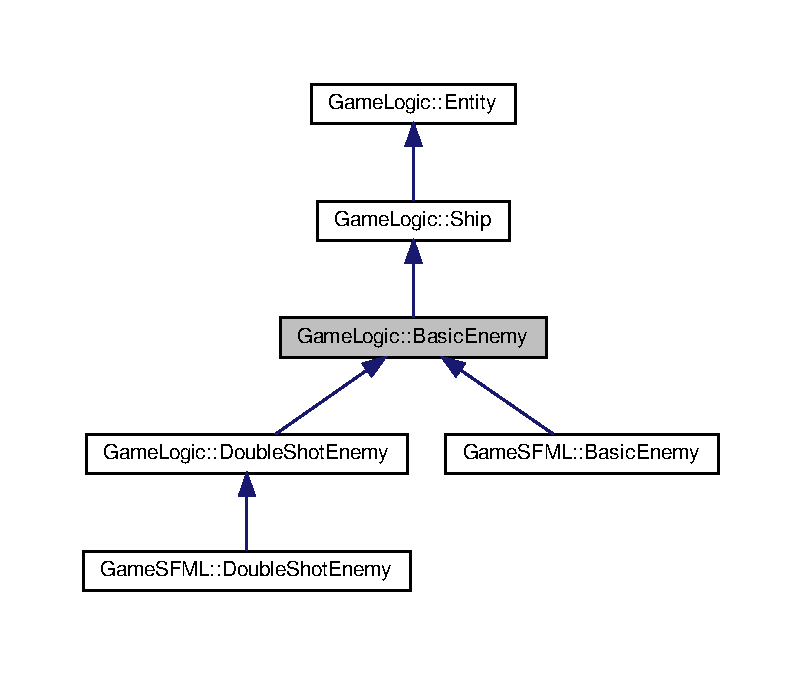
\includegraphics[width=350pt]{classGameLogic_1_1BasicEnemy__inherit__graph}
\end{center}
\end{figure}


Collaboration diagram for Game\+Logic\+:\+:Basic\+Enemy\+:\nopagebreak
\begin{figure}[H]
\begin{center}
\leavevmode
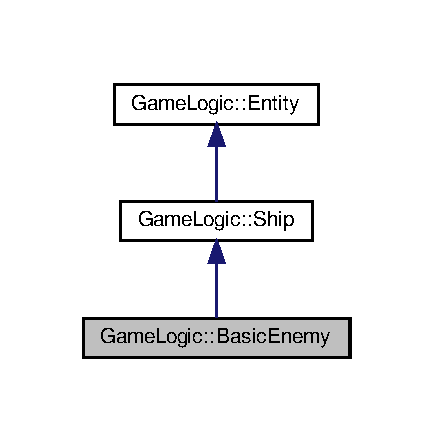
\includegraphics[width=208pt]{classGameLogic_1_1BasicEnemy__coll__graph}
\end{center}
\end{figure}
\subsection*{Public Member Functions}
\begin{DoxyCompactItemize}
\item 
\hyperlink{classGameLogic_1_1BasicEnemy_ac89d53201b55edcce7655e30afd204ed}{Basic\+Enemy} (const pair$<$ int, int $>$ \&position, double width, double height)
\begin{DoxyCompactList}\small\item\em Constructor of Basic Enemy. \end{DoxyCompactList}\item 
void \hyperlink{classGameLogic_1_1BasicEnemy_a8c51b862c94953e5455c04c2227b6d73}{move} () override
\begin{DoxyCompactList}\small\item\em Function that moves the Basic Enemy. \end{DoxyCompactList}\item 
bool \hyperlink{classGameLogic_1_1BasicEnemy_ada4bb368a6af13fbfb1ba83503099f2c}{can\+Shoot} ()
\begin{DoxyCompactList}\small\item\em Checks if the enemy can shoot. \end{DoxyCompactList}\item 
int \hyperlink{classGameLogic_1_1BasicEnemy_adec32036fbf44534988bcbc850a3e3a5}{generate\+Shoot\+Interval} ()
\begin{DoxyCompactList}\small\item\em Generates a random interval for when an enemy can shoot again. \end{DoxyCompactList}\item 
void \hyperlink{classGameLogic_1_1BasicEnemy_a3d01ac4181b0aaa6058d434195e68830}{handle\+Collision} (const shared\+\_\+ptr$<$ \hyperlink{classGameLogic_1_1Entity}{Entity} $>$ \&other\+Entity) override
\begin{DoxyCompactList}\small\item\em Handles what happens if the enemy collides with another entity. \end{DoxyCompactList}\end{DoxyCompactItemize}
\subsection*{Additional Inherited Members}


\subsection{Detailed Description}
\hyperlink{namespaceGameLogic}{Game\+Logic} version of the easiest, most basic enemy 

\subsection{Constructor \& Destructor Documentation}
\mbox{\Hypertarget{classGameLogic_1_1BasicEnemy_ac89d53201b55edcce7655e30afd204ed}\label{classGameLogic_1_1BasicEnemy_ac89d53201b55edcce7655e30afd204ed}} 
\index{Game\+Logic\+::\+Basic\+Enemy@{Game\+Logic\+::\+Basic\+Enemy}!Basic\+Enemy@{Basic\+Enemy}}
\index{Basic\+Enemy@{Basic\+Enemy}!Game\+Logic\+::\+Basic\+Enemy@{Game\+Logic\+::\+Basic\+Enemy}}
\subsubsection{\texorpdfstring{Basic\+Enemy()}{BasicEnemy()}}
{\footnotesize\ttfamily Game\+Logic\+::\+Basic\+Enemy\+::\+Basic\+Enemy (\begin{DoxyParamCaption}\item[{const pair$<$ int, int $>$ \&}]{position,  }\item[{double}]{width,  }\item[{double}]{height }\end{DoxyParamCaption})}

The constructor of the \hyperlink{namespaceGameLogic}{Game\+Logic} version of the Basic Enemy class. Sets the type to \hyperlink{classGameLogic_1_1BasicEnemy}{Basic\+Enemy} and gives it health and speed of 1. 
\begin{DoxyParams}{Parameters}
{\em position} & The position of the basic enemy in the grid \\
\hline
{\em width} & The width of the basic enemy \\
\hline
{\em height} & The height of the basic enemy \\
\hline
\end{DoxyParams}


\subsection{Member Function Documentation}
\mbox{\Hypertarget{classGameLogic_1_1BasicEnemy_ada4bb368a6af13fbfb1ba83503099f2c}\label{classGameLogic_1_1BasicEnemy_ada4bb368a6af13fbfb1ba83503099f2c}} 
\index{Game\+Logic\+::\+Basic\+Enemy@{Game\+Logic\+::\+Basic\+Enemy}!can\+Shoot@{can\+Shoot}}
\index{can\+Shoot@{can\+Shoot}!Game\+Logic\+::\+Basic\+Enemy@{Game\+Logic\+::\+Basic\+Enemy}}
\subsubsection{\texorpdfstring{can\+Shoot()}{canShoot()}}
{\footnotesize\ttfamily bool Game\+Logic\+::\+Basic\+Enemy\+::can\+Shoot (\begin{DoxyParamCaption}{ }\end{DoxyParamCaption})}

Checks if the enemy can shoot. \begin{DoxyReturn}{Returns}
True if the enemy can shoot. 
\end{DoxyReturn}
\mbox{\Hypertarget{classGameLogic_1_1BasicEnemy_adec32036fbf44534988bcbc850a3e3a5}\label{classGameLogic_1_1BasicEnemy_adec32036fbf44534988bcbc850a3e3a5}} 
\index{Game\+Logic\+::\+Basic\+Enemy@{Game\+Logic\+::\+Basic\+Enemy}!generate\+Shoot\+Interval@{generate\+Shoot\+Interval}}
\index{generate\+Shoot\+Interval@{generate\+Shoot\+Interval}!Game\+Logic\+::\+Basic\+Enemy@{Game\+Logic\+::\+Basic\+Enemy}}
\subsubsection{\texorpdfstring{generate\+Shoot\+Interval()}{generateShootInterval()}}
{\footnotesize\ttfamily int Game\+Logic\+::\+Basic\+Enemy\+::generate\+Shoot\+Interval (\begin{DoxyParamCaption}{ }\end{DoxyParamCaption})}

Generates a random interval for when an enemy can shoot again. \begin{DoxyReturn}{Returns}
the random interval between 20 and 100 
\end{DoxyReturn}
\mbox{\Hypertarget{classGameLogic_1_1BasicEnemy_a3d01ac4181b0aaa6058d434195e68830}\label{classGameLogic_1_1BasicEnemy_a3d01ac4181b0aaa6058d434195e68830}} 
\index{Game\+Logic\+::\+Basic\+Enemy@{Game\+Logic\+::\+Basic\+Enemy}!handle\+Collision@{handle\+Collision}}
\index{handle\+Collision@{handle\+Collision}!Game\+Logic\+::\+Basic\+Enemy@{Game\+Logic\+::\+Basic\+Enemy}}
\subsubsection{\texorpdfstring{handle\+Collision()}{handleCollision()}}
{\footnotesize\ttfamily void Game\+Logic\+::\+Basic\+Enemy\+::handle\+Collision (\begin{DoxyParamCaption}\item[{const shared\+\_\+ptr$<$ \hyperlink{classGameLogic_1_1Entity}{Entity} $>$ \&}]{other\+Entity }\end{DoxyParamCaption})\hspace{0.3cm}{\ttfamily [override]}, {\ttfamily [virtual]}}

Handles what happens if the enemy collides with another entity. 
\begin{DoxyParams}{Parameters}
{\em other\+Entity} & the other entity it collides with. \\
\hline
\end{DoxyParams}


Reimplemented from \hyperlink{classGameLogic_1_1Entity_af3461a4c6321b1af250821d7a1329ba7}{Game\+Logic\+::\+Entity}.

\mbox{\Hypertarget{classGameLogic_1_1BasicEnemy_a8c51b862c94953e5455c04c2227b6d73}\label{classGameLogic_1_1BasicEnemy_a8c51b862c94953e5455c04c2227b6d73}} 
\index{Game\+Logic\+::\+Basic\+Enemy@{Game\+Logic\+::\+Basic\+Enemy}!move@{move}}
\index{move@{move}!Game\+Logic\+::\+Basic\+Enemy@{Game\+Logic\+::\+Basic\+Enemy}}
\subsubsection{\texorpdfstring{move()}{move()}}
{\footnotesize\ttfamily void Game\+Logic\+::\+Basic\+Enemy\+::move (\begin{DoxyParamCaption}{ }\end{DoxyParamCaption})\hspace{0.3cm}{\ttfamily [override]}, {\ttfamily [virtual]}}

Function that moves the Basic Enemy to it\textquotesingle{}s next position in the grid and updates movingX and movingY. The Basic Enemy moves from left to right, then lowers a row before moving from right to left. It then lowers a row again before moving from left to right again. 

Reimplemented from \hyperlink{classGameLogic_1_1Ship_aaab731578b80b9e1920e3f2af2bc2f8c}{Game\+Logic\+::\+Ship}.



The documentation for this class was generated from the following files\+:\begin{DoxyCompactItemize}
\item 
Game\+Logic/\+Include/\+Game\+Logic/Basic\+Enemy.\+h\item 
Game\+Logic/src/Basic\+Enemy.\+cpp\end{DoxyCompactItemize}

\hypertarget{classGameSFML_1_1BasicEnemy}{}\section{Game\+S\+F\+ML\+:\+:Basic\+Enemy Class Reference}
\label{classGameSFML_1_1BasicEnemy}\index{Game\+S\+F\+M\+L\+::\+Basic\+Enemy@{Game\+S\+F\+M\+L\+::\+Basic\+Enemy}}


S\+F\+ML version of the \hyperlink{classGameSFML_1_1BasicEnemy}{Basic\+Enemy} class.  




{\ttfamily \#include $<$Basic\+Enemy.\+h$>$}



Inheritance diagram for Game\+S\+F\+ML\+:\+:Basic\+Enemy\+:\nopagebreak
\begin{figure}[H]
\begin{center}
\leavevmode
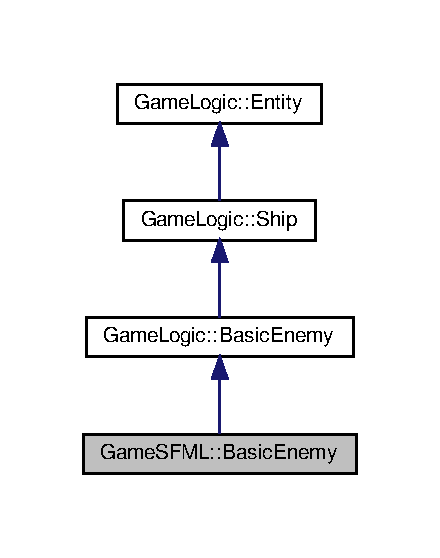
\includegraphics[width=211pt]{classGameSFML_1_1BasicEnemy__inherit__graph}
\end{center}
\end{figure}


Collaboration diagram for Game\+S\+F\+ML\+:\+:Basic\+Enemy\+:\nopagebreak
\begin{figure}[H]
\begin{center}
\leavevmode
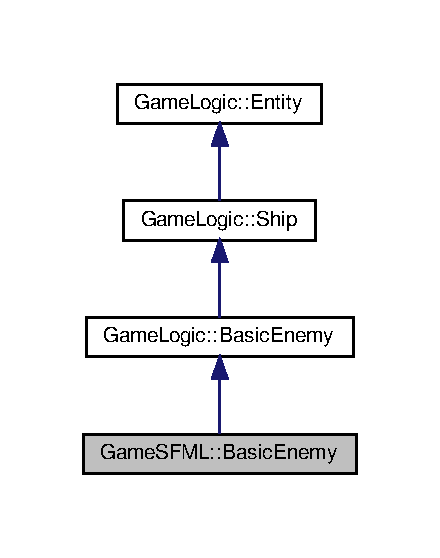
\includegraphics[width=211pt]{classGameSFML_1_1BasicEnemy__coll__graph}
\end{center}
\end{figure}
\subsection*{Public Member Functions}
\begin{DoxyCompactItemize}
\item 
\hyperlink{classGameSFML_1_1BasicEnemy_a33fe286fc3101188696952c84f6a0592}{Basic\+Enemy} (const pair$<$ int, int $>$ \&position, double width, double height, const string \&file\+Name, Game\+S\+F\+M\+L\+::window\+\_\+ptr window)
\begin{DoxyCompactList}\small\item\em Constructor of the S\+F\+ML version of Basic Enemy. \end{DoxyCompactList}\item 
void \hyperlink{classGameSFML_1_1BasicEnemy_a1062ddf1321edb7d069b68b396615626}{draw} () override
\begin{DoxyCompactList}\small\item\em Updates the sprite and draws it to the window. \end{DoxyCompactList}\item 
void \hyperlink{classGameSFML_1_1BasicEnemy_abd16a66e14ffd7067f6e397290a82198}{update\+Sprite} ()
\begin{DoxyCompactList}\small\item\em Updates the sprite to the current position. \end{DoxyCompactList}\end{DoxyCompactItemize}
\subsection*{Additional Inherited Members}


\subsection{Detailed Description}
S\+F\+ML version of the \hyperlink{classGameSFML_1_1BasicEnemy}{Basic\+Enemy} class. 

\subsection{Constructor \& Destructor Documentation}
\mbox{\Hypertarget{classGameSFML_1_1BasicEnemy_a33fe286fc3101188696952c84f6a0592}\label{classGameSFML_1_1BasicEnemy_a33fe286fc3101188696952c84f6a0592}} 
\index{Game\+S\+F\+M\+L\+::\+Basic\+Enemy@{Game\+S\+F\+M\+L\+::\+Basic\+Enemy}!Basic\+Enemy@{Basic\+Enemy}}
\index{Basic\+Enemy@{Basic\+Enemy}!Game\+S\+F\+M\+L\+::\+Basic\+Enemy@{Game\+S\+F\+M\+L\+::\+Basic\+Enemy}}
\subsubsection{\texorpdfstring{Basic\+Enemy()}{BasicEnemy()}}
{\footnotesize\ttfamily Game\+S\+F\+M\+L\+::\+Basic\+Enemy\+::\+Basic\+Enemy (\begin{DoxyParamCaption}\item[{const pair$<$ int, int $>$ \&}]{position,  }\item[{double}]{width,  }\item[{double}]{height,  }\item[{const string \&}]{file\+Name,  }\item[{Game\+S\+F\+M\+L\+::window\+\_\+ptr}]{window }\end{DoxyParamCaption})}

Constructor of the S\+F\+ML version of Basic Enemy. 
\begin{DoxyParams}{Parameters}
{\em position} & The position of the basic enemy in the grid \\
\hline
{\em width} & The width of the basic enemy \\
\hline
{\em height} & The height of the basic enemy \\
\hline
{\em file\+Name} & The name of the file that contains the sprite \\
\hline
{\em window} & The current game window. \\
\hline
\end{DoxyParams}


\subsection{Member Function Documentation}
\mbox{\Hypertarget{classGameSFML_1_1BasicEnemy_a1062ddf1321edb7d069b68b396615626}\label{classGameSFML_1_1BasicEnemy_a1062ddf1321edb7d069b68b396615626}} 
\index{Game\+S\+F\+M\+L\+::\+Basic\+Enemy@{Game\+S\+F\+M\+L\+::\+Basic\+Enemy}!draw@{draw}}
\index{draw@{draw}!Game\+S\+F\+M\+L\+::\+Basic\+Enemy@{Game\+S\+F\+M\+L\+::\+Basic\+Enemy}}
\subsubsection{\texorpdfstring{draw()}{draw()}}
{\footnotesize\ttfamily void Game\+S\+F\+M\+L\+::\+Basic\+Enemy\+::draw (\begin{DoxyParamCaption}{ }\end{DoxyParamCaption})\hspace{0.3cm}{\ttfamily [override]}, {\ttfamily [virtual]}}

Updates the sprite and draws it to the window. 

Implements \hyperlink{classGameLogic_1_1Entity_adf23a7036cb99dfc6e33434018131da4}{Game\+Logic\+::\+Entity}.

\mbox{\Hypertarget{classGameSFML_1_1BasicEnemy_abd16a66e14ffd7067f6e397290a82198}\label{classGameSFML_1_1BasicEnemy_abd16a66e14ffd7067f6e397290a82198}} 
\index{Game\+S\+F\+M\+L\+::\+Basic\+Enemy@{Game\+S\+F\+M\+L\+::\+Basic\+Enemy}!update\+Sprite@{update\+Sprite}}
\index{update\+Sprite@{update\+Sprite}!Game\+S\+F\+M\+L\+::\+Basic\+Enemy@{Game\+S\+F\+M\+L\+::\+Basic\+Enemy}}
\subsubsection{\texorpdfstring{update\+Sprite()}{updateSprite()}}
{\footnotesize\ttfamily void Game\+S\+F\+M\+L\+::\+Basic\+Enemy\+::update\+Sprite (\begin{DoxyParamCaption}{ }\end{DoxyParamCaption})}

Updates the sprite to the current position. 

The documentation for this class was generated from the following files\+:\begin{DoxyCompactItemize}
\item 
S\+F\+M\+L/\+Include/Basic\+Enemy.\+h\item 
S\+F\+M\+L/src/Basic\+Enemy.\+cpp\end{DoxyCompactItemize}

\hypertarget{classGameLogic_1_1BasicEnemyBullet}{}\section{Game\+Logic\+:\+:Basic\+Enemy\+Bullet Class Reference}
\label{classGameLogic_1_1BasicEnemyBullet}\index{Game\+Logic\+::\+Basic\+Enemy\+Bullet@{Game\+Logic\+::\+Basic\+Enemy\+Bullet}}


\hyperlink{namespaceGameLogic}{Game\+Logic} version of \hyperlink{classGameLogic_1_1BasicEnemyBullet}{Basic\+Enemy\+Bullet}.  




{\ttfamily \#include $<$Basic\+Enemy\+Bullet.\+h$>$}



Inheritance diagram for Game\+Logic\+:\+:Basic\+Enemy\+Bullet\+:
\nopagebreak
\begin{figure}[H]
\begin{center}
\leavevmode
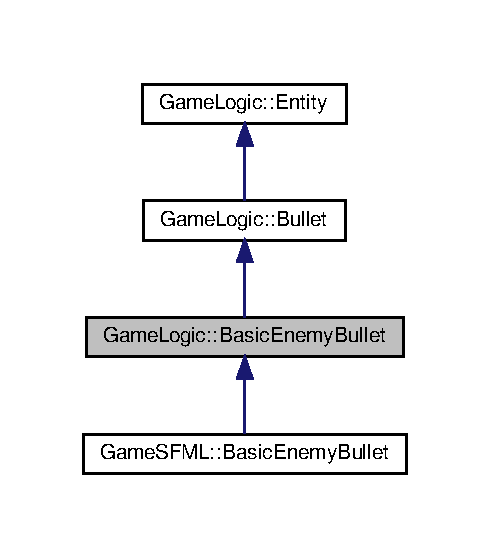
\includegraphics[width=235pt]{classGameLogic_1_1BasicEnemyBullet__inherit__graph}
\end{center}
\end{figure}


Collaboration diagram for Game\+Logic\+:\+:Basic\+Enemy\+Bullet\+:
\nopagebreak
\begin{figure}[H]
\begin{center}
\leavevmode
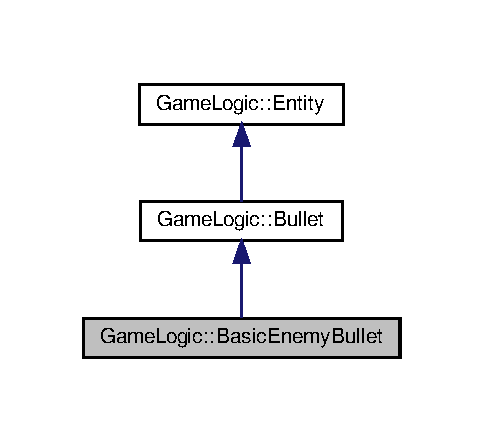
\includegraphics[width=232pt]{classGameLogic_1_1BasicEnemyBullet__coll__graph}
\end{center}
\end{figure}
\subsection*{Public Member Functions}
\begin{DoxyCompactItemize}
\item 
\hyperlink{classGameLogic_1_1BasicEnemyBullet_a7c6a8feb4edd34089738f1e9c54d31d2}{Basic\+Enemy\+Bullet} (const pair$<$ int, int $>$ \&position, double width, double height)
\begin{DoxyCompactList}\small\item\em Constructor for the Game Logic version of \hyperlink{classGameLogic_1_1BasicEnemyBullet}{Basic\+Enemy\+Bullet}. \end{DoxyCompactList}\item 
void \hyperlink{classGameLogic_1_1BasicEnemyBullet_a220f79a5cb5bfb33e63ad232457bad54}{handle\+Collision} (const shared\+\_\+ptr$<$ \hyperlink{classGameLogic_1_1Entity}{Entity} $>$ \&other\+Entity) override
\begin{DoxyCompactList}\small\item\em Handles what happens if the bullet collides with another entity. \end{DoxyCompactList}\end{DoxyCompactItemize}
\subsection*{Additional Inherited Members}


\subsection{Detailed Description}
\hyperlink{namespaceGameLogic}{Game\+Logic} version of \hyperlink{classGameLogic_1_1BasicEnemyBullet}{Basic\+Enemy\+Bullet}. 

\subsection{Constructor \& Destructor Documentation}
\mbox{\Hypertarget{classGameLogic_1_1BasicEnemyBullet_a7c6a8feb4edd34089738f1e9c54d31d2}\label{classGameLogic_1_1BasicEnemyBullet_a7c6a8feb4edd34089738f1e9c54d31d2}} 
\index{Game\+Logic\+::\+Basic\+Enemy\+Bullet@{Game\+Logic\+::\+Basic\+Enemy\+Bullet}!Basic\+Enemy\+Bullet@{Basic\+Enemy\+Bullet}}
\index{Basic\+Enemy\+Bullet@{Basic\+Enemy\+Bullet}!Game\+Logic\+::\+Basic\+Enemy\+Bullet@{Game\+Logic\+::\+Basic\+Enemy\+Bullet}}
\subsubsection{\texorpdfstring{Basic\+Enemy\+Bullet()}{BasicEnemyBullet()}}
{\footnotesize\ttfamily Game\+Logic\+::\+Basic\+Enemy\+Bullet\+::\+Basic\+Enemy\+Bullet (\begin{DoxyParamCaption}\item[{const pair$<$ int, int $>$ \&}]{position,  }\item[{double}]{width,  }\item[{double}]{height }\end{DoxyParamCaption})}

Constructor for the Game Logic version of \hyperlink{classGameLogic_1_1BasicEnemyBullet}{Basic\+Enemy\+Bullet}. 
\begin{DoxyParams}{Parameters}
{\em position} & the starting position of the bullet \\
\hline
{\em width} & the width of the bullet. \\
\hline
{\em height} & the height of the bullet. \\
\hline
\end{DoxyParams}


\subsection{Member Function Documentation}
\mbox{\Hypertarget{classGameLogic_1_1BasicEnemyBullet_a220f79a5cb5bfb33e63ad232457bad54}\label{classGameLogic_1_1BasicEnemyBullet_a220f79a5cb5bfb33e63ad232457bad54}} 
\index{Game\+Logic\+::\+Basic\+Enemy\+Bullet@{Game\+Logic\+::\+Basic\+Enemy\+Bullet}!handle\+Collision@{handle\+Collision}}
\index{handle\+Collision@{handle\+Collision}!Game\+Logic\+::\+Basic\+Enemy\+Bullet@{Game\+Logic\+::\+Basic\+Enemy\+Bullet}}
\subsubsection{\texorpdfstring{handle\+Collision()}{handleCollision()}}
{\footnotesize\ttfamily void Game\+Logic\+::\+Basic\+Enemy\+Bullet\+::handle\+Collision (\begin{DoxyParamCaption}\item[{const shared\+\_\+ptr$<$ \hyperlink{classGameLogic_1_1Entity}{Entity} $>$ \&}]{other\+Entity }\end{DoxyParamCaption})\hspace{0.3cm}{\ttfamily [override]}, {\ttfamily [virtual]}}

Handles what happens if the bullet collides with another entity. 
\begin{DoxyParams}{Parameters}
{\em other\+Entity} & the other entity it collides with. \\
\hline
\end{DoxyParams}


Reimplemented from \hyperlink{classGameLogic_1_1Entity_af3461a4c6321b1af250821d7a1329ba7}{Game\+Logic\+::\+Entity}.



The documentation for this class was generated from the following files\+:\begin{DoxyCompactItemize}
\item 
Game\+Logic/\+Include/\+Game\+Logic/Basic\+Enemy\+Bullet.\+h\item 
Game\+Logic/src/Basic\+Enemy\+Bullet.\+cpp\end{DoxyCompactItemize}

\hypertarget{classGameSFML_1_1BasicEnemyBullet}{}\section{Game\+S\+F\+ML\+:\+:Basic\+Enemy\+Bullet Class Reference}
\label{classGameSFML_1_1BasicEnemyBullet}\index{Game\+S\+F\+M\+L\+::\+Basic\+Enemy\+Bullet@{Game\+S\+F\+M\+L\+::\+Basic\+Enemy\+Bullet}}


S\+F\+ML version of the basic\+Enemy\+Bullet class.  




{\ttfamily \#include $<$Basic\+Enemy\+Bullet.\+h$>$}



Inheritance diagram for Game\+S\+F\+ML\+:\+:Basic\+Enemy\+Bullet\+:
\nopagebreak
\begin{figure}[H]
\begin{center}
\leavevmode
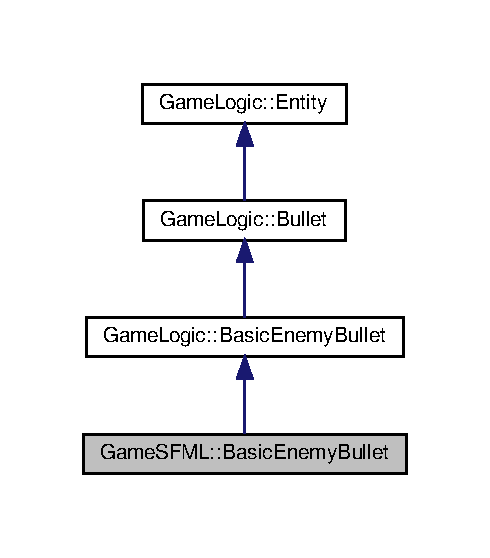
\includegraphics[width=235pt]{classGameSFML_1_1BasicEnemyBullet__inherit__graph}
\end{center}
\end{figure}


Collaboration diagram for Game\+S\+F\+ML\+:\+:Basic\+Enemy\+Bullet\+:
\nopagebreak
\begin{figure}[H]
\begin{center}
\leavevmode
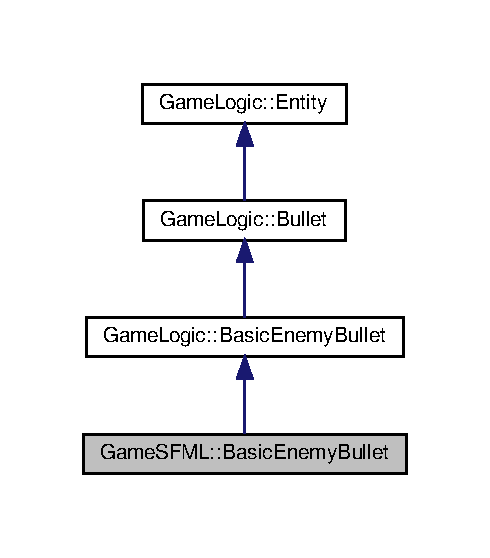
\includegraphics[width=235pt]{classGameSFML_1_1BasicEnemyBullet__coll__graph}
\end{center}
\end{figure}
\subsection*{Public Member Functions}
\begin{DoxyCompactItemize}
\item 
\hyperlink{classGameSFML_1_1BasicEnemyBullet_aa2daeed3aec6be3661879afaae0855d1}{Basic\+Enemy\+Bullet} (const pair$<$ int, int $>$ \&position, double width, double height, const string \&file\+Name, const window\+\_\+ptr \&window)
\begin{DoxyCompactList}\small\item\em Constructor of the S\+F\+ML \hyperlink{classGameSFML_1_1BasicEnemyBullet}{Basic\+Enemy\+Bullet}. \end{DoxyCompactList}\item 
void \hyperlink{classGameSFML_1_1BasicEnemyBullet_af970b7b86c5a21963daac86822a064a2}{draw} () override
\begin{DoxyCompactList}\small\item\em Updates the sprite and draws it to the window. \end{DoxyCompactList}\item 
void \hyperlink{classGameSFML_1_1BasicEnemyBullet_a12e639b51bc2212fd35af3d8fb0bbb56}{update\+Sprite} ()
\begin{DoxyCompactList}\small\item\em Updates the sprite to the current position. \end{DoxyCompactList}\end{DoxyCompactItemize}
\subsection*{Additional Inherited Members}


\subsection{Detailed Description}
S\+F\+ML version of the Basic Enemy\textquotesingle{}s bullet. 

\subsection{Constructor \& Destructor Documentation}
\mbox{\Hypertarget{classGameSFML_1_1BasicEnemyBullet_aa2daeed3aec6be3661879afaae0855d1}\label{classGameSFML_1_1BasicEnemyBullet_aa2daeed3aec6be3661879afaae0855d1}} 
\index{Game\+S\+F\+M\+L\+::\+Basic\+Enemy\+Bullet@{Game\+S\+F\+M\+L\+::\+Basic\+Enemy\+Bullet}!Basic\+Enemy\+Bullet@{Basic\+Enemy\+Bullet}}
\index{Basic\+Enemy\+Bullet@{Basic\+Enemy\+Bullet}!Game\+S\+F\+M\+L\+::\+Basic\+Enemy\+Bullet@{Game\+S\+F\+M\+L\+::\+Basic\+Enemy\+Bullet}}
\subsubsection{\texorpdfstring{Basic\+Enemy\+Bullet()}{BasicEnemyBullet()}}
{\footnotesize\ttfamily Game\+S\+F\+M\+L\+::\+Basic\+Enemy\+Bullet\+::\+Basic\+Enemy\+Bullet (\begin{DoxyParamCaption}\item[{const pair$<$ int, int $>$ \&}]{position,  }\item[{double}]{width,  }\item[{double}]{height,  }\item[{const string \&}]{file\+Name,  }\item[{const window\+\_\+ptr \&}]{window }\end{DoxyParamCaption})}

Constructor of the S\+F\+ML \hyperlink{classGameSFML_1_1BasicEnemyBullet}{Basic\+Enemy\+Bullet}. 
\begin{DoxyParams}{Parameters}
{\em position} & Position in the grid of the bullet \\
\hline
{\em width} & width of the bullet \\
\hline
{\em height} & height of the bullet \\
\hline
{\em file\+Name} & name of the file of the sprite of the bullet \\
\hline
{\em window} & current game window \\
\hline
\end{DoxyParams}


\subsection{Member Function Documentation}
\mbox{\Hypertarget{classGameSFML_1_1BasicEnemyBullet_af970b7b86c5a21963daac86822a064a2}\label{classGameSFML_1_1BasicEnemyBullet_af970b7b86c5a21963daac86822a064a2}} 
\index{Game\+S\+F\+M\+L\+::\+Basic\+Enemy\+Bullet@{Game\+S\+F\+M\+L\+::\+Basic\+Enemy\+Bullet}!draw@{draw}}
\index{draw@{draw}!Game\+S\+F\+M\+L\+::\+Basic\+Enemy\+Bullet@{Game\+S\+F\+M\+L\+::\+Basic\+Enemy\+Bullet}}
\subsubsection{\texorpdfstring{draw()}{draw()}}
{\footnotesize\ttfamily void Game\+S\+F\+M\+L\+::\+Basic\+Enemy\+Bullet\+::draw (\begin{DoxyParamCaption}{ }\end{DoxyParamCaption})\hspace{0.3cm}{\ttfamily [override]}, {\ttfamily [virtual]}}

Updates the sprite and draws it to the window. 

Implements \hyperlink{classGameLogic_1_1Entity_adf23a7036cb99dfc6e33434018131da4}{Game\+Logic\+::\+Entity}.

\mbox{\Hypertarget{classGameSFML_1_1BasicEnemyBullet_a12e639b51bc2212fd35af3d8fb0bbb56}\label{classGameSFML_1_1BasicEnemyBullet_a12e639b51bc2212fd35af3d8fb0bbb56}} 
\index{Game\+S\+F\+M\+L\+::\+Basic\+Enemy\+Bullet@{Game\+S\+F\+M\+L\+::\+Basic\+Enemy\+Bullet}!update\+Sprite@{update\+Sprite}}
\index{update\+Sprite@{update\+Sprite}!Game\+S\+F\+M\+L\+::\+Basic\+Enemy\+Bullet@{Game\+S\+F\+M\+L\+::\+Basic\+Enemy\+Bullet}}
\subsubsection{\texorpdfstring{update\+Sprite()}{updateSprite()}}
{\footnotesize\ttfamily void Game\+S\+F\+M\+L\+::\+Basic\+Enemy\+Bullet\+::update\+Sprite (\begin{DoxyParamCaption}{ }\end{DoxyParamCaption})}

Updates the sprite to the current position. 

The documentation for this class was generated from the following files\+:\begin{DoxyCompactItemize}
\item 
S\+F\+M\+L/\+Include/Basic\+Enemy\+Bullet.\+h\item 
S\+F\+M\+L/src/Basic\+Enemy\+Bullet.\+cpp\end{DoxyCompactItemize}

\hypertarget{classGameLogic_1_1Bullet}{}\section{Game\+Logic\+:\+:Bullet Class Reference}
\label{classGameLogic_1_1Bullet}\index{Game\+Logic\+::\+Bullet@{Game\+Logic\+::\+Bullet}}


Class to represent all bullet types in game.  




{\ttfamily \#include $<$Bullet.\+h$>$}



Inheritance diagram for Game\+Logic\+:\+:Bullet\+:
\nopagebreak
\begin{figure}[H]
\begin{center}
\leavevmode
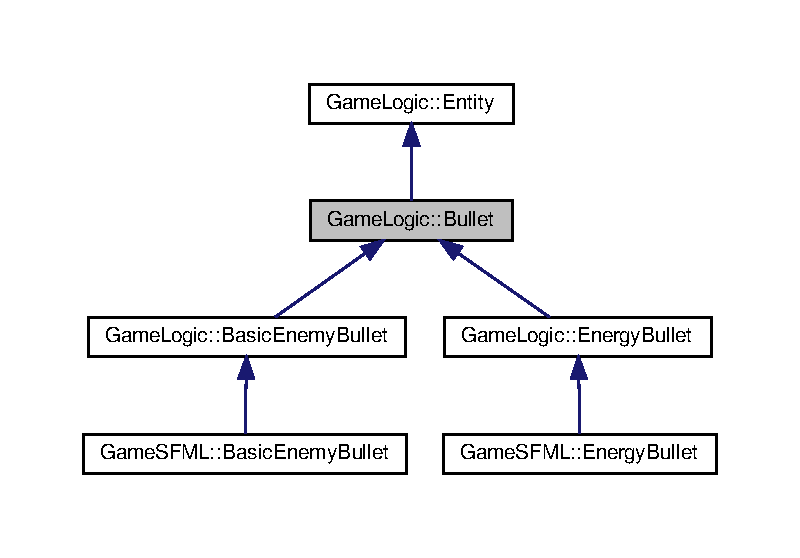
\includegraphics[width=350pt]{classGameLogic_1_1Bullet__inherit__graph}
\end{center}
\end{figure}


Collaboration diagram for Game\+Logic\+:\+:Bullet\+:\nopagebreak
\begin{figure}[H]
\begin{center}
\leavevmode
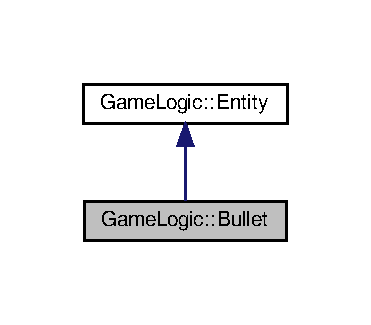
\includegraphics[width=178pt]{classGameLogic_1_1Bullet__coll__graph}
\end{center}
\end{figure}
\subsection*{Public Member Functions}
\begin{DoxyCompactItemize}
\item 
\hyperlink{classGameLogic_1_1Bullet_a1a9519e2cd64746d3e545d45734ffddf}{Bullet} (const pair$<$ int, int $>$ \&position, double width=64, double height=64)
\begin{DoxyCompactList}\small\item\em Constructor for \hyperlink{classGameLogic_1_1Bullet}{Bullet} class. \end{DoxyCompactList}\item 
void \hyperlink{classGameLogic_1_1Bullet_a8581833f7a73cef83411fa988f6fe94d}{move} ()
\begin{DoxyCompactList}\small\item\em Virtual function determines what happens when the bullet hits an \hyperlink{classGameLogic_1_1Entity}{Entity}. \end{DoxyCompactList}\end{DoxyCompactItemize}
\subsection*{Additional Inherited Members}


\subsection{Detailed Description}
Class to represent all bullet types in game. 

\subsection{Constructor \& Destructor Documentation}
\mbox{\Hypertarget{classGameLogic_1_1Bullet_a1a9519e2cd64746d3e545d45734ffddf}\label{classGameLogic_1_1Bullet_a1a9519e2cd64746d3e545d45734ffddf}} 
\index{Game\+Logic\+::\+Bullet@{Game\+Logic\+::\+Bullet}!Bullet@{Bullet}}
\index{Bullet@{Bullet}!Game\+Logic\+::\+Bullet@{Game\+Logic\+::\+Bullet}}
\subsubsection{\texorpdfstring{Bullet()}{Bullet()}}
{\footnotesize\ttfamily Game\+Logic\+::\+Bullet\+::\+Bullet (\begin{DoxyParamCaption}\item[{const pair$<$ int, int $>$ \&}]{position,  }\item[{double}]{width = {\ttfamily 64},  }\item[{double}]{height = {\ttfamily 64} }\end{DoxyParamCaption})\hspace{0.3cm}{\ttfamily [explicit]}}

Constructor for \hyperlink{classGameLogic_1_1Bullet}{Bullet} class. 
\begin{DoxyParams}{Parameters}
{\em position} & the starting position of the bullet \\
\hline
{\em width} & the width of the bullet. \\
\hline
{\em height} & the height of the bullet. \\
\hline
\end{DoxyParams}


\subsection{Member Function Documentation}
\mbox{\Hypertarget{classGameLogic_1_1Bullet_a8581833f7a73cef83411fa988f6fe94d}\label{classGameLogic_1_1Bullet_a8581833f7a73cef83411fa988f6fe94d}} 
\index{Game\+Logic\+::\+Bullet@{Game\+Logic\+::\+Bullet}!move@{move}}
\index{move@{move}!Game\+Logic\+::\+Bullet@{Game\+Logic\+::\+Bullet}}
\subsubsection{\texorpdfstring{move()}{move()}}
{\footnotesize\ttfamily void Game\+Logic\+::\+Bullet\+::move (\begin{DoxyParamCaption}{ }\end{DoxyParamCaption})}

Function determines what happens when the bullet hits an \hyperlink{classGameLogic_1_1Entity}{Entity}. What exactly happens depends on the type of bullet and the type of \hyperlink{classGameLogic_1_1Entity}{Entity}. 
\begin{DoxyParams}{Parameters}
{\em hit\+Entity} & Shared\+\_\+ptr to the \hyperlink{classGameLogic_1_1Entity}{Entity} that was hit. Moves the bullet up or down according to speed. Moves the bullet up or down according to speed. \\
\hline
\end{DoxyParams}


The documentation for this class was generated from the following files\+:\begin{DoxyCompactItemize}
\item 
Game\+Logic/\+Include/\+Game\+Logic/Bullet.\+h\item 
Game\+Logic/src/Bullet.\+cpp\end{DoxyCompactItemize}

\hypertarget{classController}{}\section{Controller Class Reference}
\label{classController}\index{Controller@{Controller}}


\hyperlink{classController}{Controller} class.  




{\ttfamily \#include $<$Controller.\+h$>$}

\subsection*{Public Member Functions}
\begin{DoxyCompactItemize}
\item 
void \hyperlink{classController_aa89ab5fe861da53f35c48f03005486de}{set\+Current\+Level} (shared\+\_\+ptr$<$ \hyperlink{classGameSFML_1_1Level}{Game\+S\+F\+M\+L\+::\+Level} $>$ new\+Level)
\begin{DoxyCompactList}\small\item\em Setter for the current level in the game. \end{DoxyCompactList}\item 
void \hyperlink{classController_a6ecc2df639760a276d0b9bf2f05ad3ab}{set\+Window} (shared\+\_\+ptr$<$ sf\+::\+Render\+Window $>$ window)
\begin{DoxyCompactList}\small\item\em Setter for the current game window. \end{DoxyCompactList}\item 
void \hyperlink{classController_aa8caf600ecfb41c59da3df61cd1291b2}{handle\+Input} ()
\begin{DoxyCompactList}\small\item\em Main function to handle input. \end{DoxyCompactList}\item 
void \hyperlink{classController_a3742c489d3d26781155fcb7c06b6dfaa}{initialize\+Level} (int level\+Number)
\begin{DoxyCompactList}\small\item\em Initialize a new level in the game. \end{DoxyCompactList}\item 
shared\+\_\+ptr$<$ \hyperlink{classGameSFML_1_1Level}{Game\+S\+F\+M\+L\+::\+Level} $>$ \& \hyperlink{classController_ad4126984329d864fcd63b10103c6e138}{get\+Current\+Level} ()
\begin{DoxyCompactList}\small\item\em Getter for the current level. \end{DoxyCompactList}\end{DoxyCompactItemize}
\subsection*{Static Public Member Functions}
\begin{DoxyCompactItemize}
\item 
static shared\+\_\+ptr$<$ \hyperlink{classController}{Controller} $>$ \hyperlink{classController_a155147647e348dc4c805977e93889512}{get\+Instance} ()
\begin{DoxyCompactList}\small\item\em Function to get the controller instance. \end{DoxyCompactList}\end{DoxyCompactItemize}


\subsection{Detailed Description}
This class will handle all input of the game. Works on the singleton priciple so only one controller is always active. 

\subsection{Member Function Documentation}
\mbox{\Hypertarget{classController_ad4126984329d864fcd63b10103c6e138}\label{classController_ad4126984329d864fcd63b10103c6e138}} 
\index{Controller@{Controller}!get\+Current\+Level@{get\+Current\+Level}}
\index{get\+Current\+Level@{get\+Current\+Level}!Controller@{Controller}}
\subsubsection{\texorpdfstring{get\+Current\+Level()}{getCurrentLevel()}}
{\footnotesize\ttfamily shared\+\_\+ptr$<$ \hyperlink{classGameSFML_1_1Level}{Game\+S\+F\+M\+L\+::\+Level} $>$ \& Controller\+::get\+Current\+Level (\begin{DoxyParamCaption}{ }\end{DoxyParamCaption})}

Getter for the current level. \begin{DoxyReturn}{Returns}
the current level. 
\end{DoxyReturn}
\mbox{\Hypertarget{classController_a155147647e348dc4c805977e93889512}\label{classController_a155147647e348dc4c805977e93889512}} 
\index{Controller@{Controller}!get\+Instance@{get\+Instance}}
\index{get\+Instance@{get\+Instance}!Controller@{Controller}}
\subsubsection{\texorpdfstring{get\+Instance()}{getInstance()}}
{\footnotesize\ttfamily shared\+\_\+ptr$<$ \hyperlink{classController}{Controller} $>$ Controller\+::get\+Instance (\begin{DoxyParamCaption}{ }\end{DoxyParamCaption})\hspace{0.3cm}{\ttfamily [static]}}

Will return the controller instance if one already exists, if not it will create one. \begin{DoxyReturn}{Returns}
The controller instance 
\end{DoxyReturn}
\mbox{\Hypertarget{classController_aa8caf600ecfb41c59da3df61cd1291b2}\label{classController_aa8caf600ecfb41c59da3df61cd1291b2}} 
\index{Controller@{Controller}!handle\+Input@{handle\+Input}}
\index{handle\+Input@{handle\+Input}!Controller@{Controller}}
\subsubsection{\texorpdfstring{handle\+Input()}{handleInput()}}
{\footnotesize\ttfamily void Controller\+::handle\+Input (\begin{DoxyParamCaption}{ }\end{DoxyParamCaption})}

Function will handle all input given to the game window and decide what to do with it, with exception of closing the window using the window\textquotesingle{}s own close button. \mbox{\Hypertarget{classController_a3742c489d3d26781155fcb7c06b6dfaa}\label{classController_a3742c489d3d26781155fcb7c06b6dfaa}} 
\index{Controller@{Controller}!initialize\+Level@{initialize\+Level}}
\index{initialize\+Level@{initialize\+Level}!Controller@{Controller}}
\subsubsection{\texorpdfstring{initialize\+Level()}{initializeLevel()}}
{\footnotesize\ttfamily void Controller\+::initialize\+Level (\begin{DoxyParamCaption}\item[{int}]{level\+Number }\end{DoxyParamCaption})}

Function initializes a new level by calling the Level Parser 
\begin{DoxyParams}{Parameters}
{\em level\+File} & the name of the json file of the new level \\
\hline
\end{DoxyParams}
\mbox{\Hypertarget{classController_aa89ab5fe861da53f35c48f03005486de}\label{classController_aa89ab5fe861da53f35c48f03005486de}} 
\index{Controller@{Controller}!set\+Current\+Level@{set\+Current\+Level}}
\index{set\+Current\+Level@{set\+Current\+Level}!Controller@{Controller}}
\subsubsection{\texorpdfstring{set\+Current\+Level()}{setCurrentLevel()}}
{\footnotesize\ttfamily void Controller\+::set\+Current\+Level (\begin{DoxyParamCaption}\item[{shared\+\_\+ptr$<$ \hyperlink{classGameSFML_1_1Level}{Game\+S\+F\+M\+L\+::\+Level} $>$}]{new\+Level }\end{DoxyParamCaption})}

Setter for the current level in the game so the controller knows which entities to affect. 
\begin{DoxyParams}{Parameters}
{\em new\+Level} & The new current level. \\
\hline
\end{DoxyParams}
\mbox{\Hypertarget{classController_a6ecc2df639760a276d0b9bf2f05ad3ab}\label{classController_a6ecc2df639760a276d0b9bf2f05ad3ab}} 
\index{Controller@{Controller}!set\+Window@{set\+Window}}
\index{set\+Window@{set\+Window}!Controller@{Controller}}
\subsubsection{\texorpdfstring{set\+Window()}{setWindow()}}
{\footnotesize\ttfamily void Controller\+::set\+Window (\begin{DoxyParamCaption}\item[{shared\+\_\+ptr$<$ sf\+::\+Render\+Window $>$}]{window }\end{DoxyParamCaption})}

Setter for the current game window so the controller knows where to get it\textquotesingle{}s input from. 
\begin{DoxyParams}{Parameters}
{\em window} & The current game window. \\
\hline
\end{DoxyParams}


The documentation for this class was generated from the following files\+:\begin{DoxyCompactItemize}
\item 
Controller.\+h\item 
Controller.\+cpp\item 
main.\+cpp\end{DoxyCompactItemize}

\hypertarget{classGameLogic_1_1DoubleShotEnemy}{}\section{Game\+Logic\+:\+:Double\+Shot\+Enemy Class Reference}
\label{classGameLogic_1_1DoubleShotEnemy}\index{Game\+Logic\+::\+Double\+Shot\+Enemy@{Game\+Logic\+::\+Double\+Shot\+Enemy}}


Class to represent the \hyperlink{classGameLogic_1_1DoubleShotEnemy}{Double\+Shot\+Enemy}.  




{\ttfamily \#include $<$Double\+Shot\+Enemy.\+h$>$}



Inheritance diagram for Game\+Logic\+:\+:Double\+Shot\+Enemy\+:
\nopagebreak
\begin{figure}[H]
\begin{center}
\leavevmode
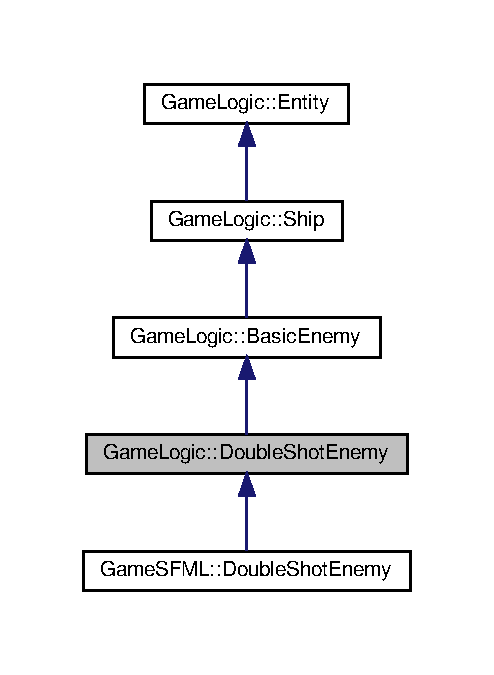
\includegraphics[width=237pt]{classGameLogic_1_1DoubleShotEnemy__inherit__graph}
\end{center}
\end{figure}


Collaboration diagram for Game\+Logic\+:\+:Double\+Shot\+Enemy\+:\nopagebreak
\begin{figure}[H]
\begin{center}
\leavevmode
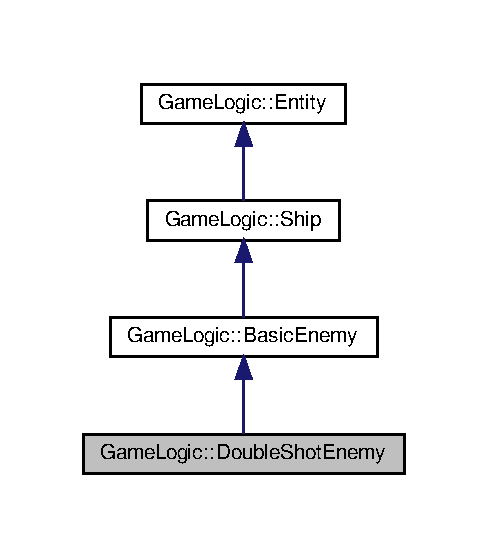
\includegraphics[width=234pt]{classGameLogic_1_1DoubleShotEnemy__coll__graph}
\end{center}
\end{figure}
\subsection*{Public Member Functions}
\begin{DoxyCompactItemize}
\item 
\hyperlink{classGameLogic_1_1DoubleShotEnemy_af5fc1cc7366c88a37696e3f8640ee88f}{Double\+Shot\+Enemy} (const pair$<$ int, int $>$ \&position, double width, double height)
\begin{DoxyCompactList}\small\item\em Constructor of the \hyperlink{classGameLogic_1_1DoubleShotEnemy}{Double\+Shot\+Enemy}. \end{DoxyCompactList}\end{DoxyCompactItemize}
\subsection*{Additional Inherited Members}


\subsection{Detailed Description}
Class to represent the \hyperlink{classGameLogic_1_1DoubleShotEnemy}{Double\+Shot\+Enemy}, a variant on the basic enemy that requires 2 shots to kill. 

\subsection{Constructor \& Destructor Documentation}
\mbox{\Hypertarget{classGameLogic_1_1DoubleShotEnemy_af5fc1cc7366c88a37696e3f8640ee88f}\label{classGameLogic_1_1DoubleShotEnemy_af5fc1cc7366c88a37696e3f8640ee88f}} 
\index{Game\+Logic\+::\+Double\+Shot\+Enemy@{Game\+Logic\+::\+Double\+Shot\+Enemy}!Double\+Shot\+Enemy@{Double\+Shot\+Enemy}}
\index{Double\+Shot\+Enemy@{Double\+Shot\+Enemy}!Game\+Logic\+::\+Double\+Shot\+Enemy@{Game\+Logic\+::\+Double\+Shot\+Enemy}}
\subsubsection{\texorpdfstring{Double\+Shot\+Enemy()}{DoubleShotEnemy()}}
{\footnotesize\ttfamily Game\+Logic\+::\+Double\+Shot\+Enemy\+::\+Double\+Shot\+Enemy (\begin{DoxyParamCaption}\item[{const pair$<$ int, int $>$ \&}]{position,  }\item[{double}]{width,  }\item[{double}]{height }\end{DoxyParamCaption})}

Constructor of the \hyperlink{classGameLogic_1_1DoubleShotEnemy}{Double\+Shot\+Enemy}. 
\begin{DoxyParams}{Parameters}
{\em position} & The position of the enemy in the grid \\
\hline
{\em width} & The width of the enemy \\
\hline
{\em height} & The height of the enemy \\
\hline
\end{DoxyParams}


The documentation for this class was generated from the following files\+:\begin{DoxyCompactItemize}
\item 
Game\+Logic/\+Include/\+Game\+Logic/Double\+Shot\+Enemy.\+h\item 
Game\+Logic/src/Double\+Shot\+Enemy.\+cpp\end{DoxyCompactItemize}

\hypertarget{classGameSFML_1_1DoubleShotEnemy}{}\section{Game\+S\+F\+ML\+:\+:Double\+Shot\+Enemy Class Reference}
\label{classGameSFML_1_1DoubleShotEnemy}\index{Game\+S\+F\+M\+L\+::\+Double\+Shot\+Enemy@{Game\+S\+F\+M\+L\+::\+Double\+Shot\+Enemy}}


S\+F\+ML version of the double\+Shot\+Enemy class.  




{\ttfamily \#include $<$Double\+Shot\+Enemy.\+h$>$}



Inheritance diagram for Game\+S\+F\+ML\+:\+:Double\+Shot\+Enemy\+:
\nopagebreak
\begin{figure}[H]
\begin{center}
\leavevmode
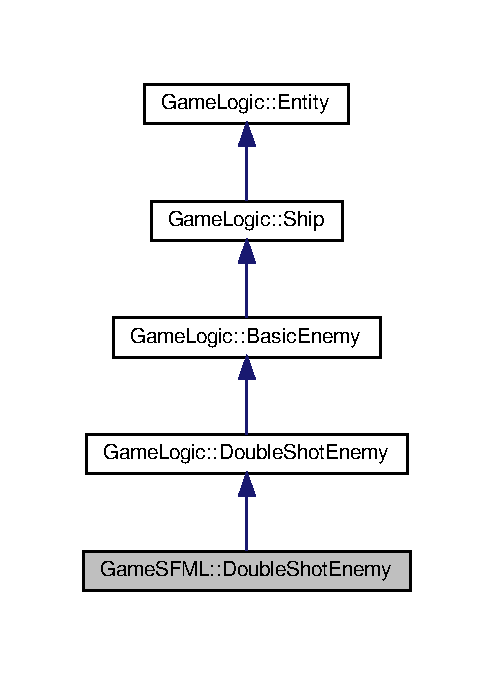
\includegraphics[width=237pt]{classGameSFML_1_1DoubleShotEnemy__inherit__graph}
\end{center}
\end{figure}


Collaboration diagram for Game\+S\+F\+ML\+:\+:Double\+Shot\+Enemy\+:
\nopagebreak
\begin{figure}[H]
\begin{center}
\leavevmode
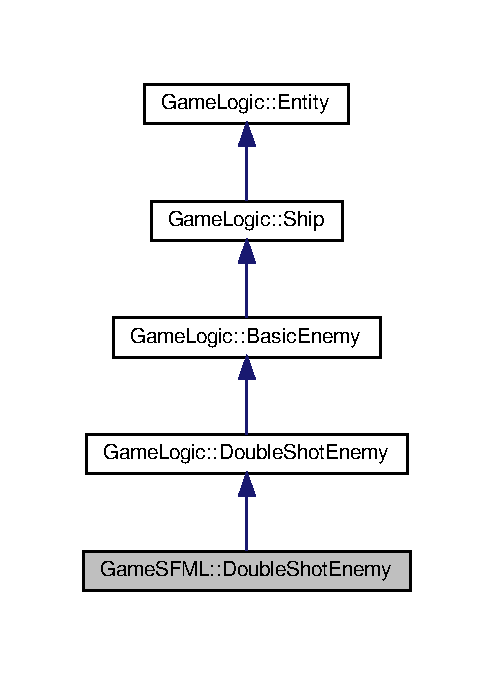
\includegraphics[width=237pt]{classGameSFML_1_1DoubleShotEnemy__coll__graph}
\end{center}
\end{figure}
\subsection*{Public Member Functions}
\begin{DoxyCompactItemize}
\item 
\hyperlink{classGameSFML_1_1DoubleShotEnemy_aac02c60e67312c1b15ccae83c4d2a4ea}{Double\+Shot\+Enemy} (const pair$<$ int, int $>$ \&position, double width, double height, const string \&file\+Name, Game\+S\+F\+M\+L\+::window\+\_\+ptr window)
\begin{DoxyCompactList}\small\item\em Constructor of the S\+F\+ML version of Double Shot Enemy. \end{DoxyCompactList}\item 
void \hyperlink{classGameSFML_1_1DoubleShotEnemy_a3d30aebbab50ad019207d6ba91ab0b5f}{draw} () override
\begin{DoxyCompactList}\small\item\em Updates the sprite and draws it to the window. \end{DoxyCompactList}\item 
void \hyperlink{classGameSFML_1_1DoubleShotEnemy_a9f93afa5fb33282829667f49f4fc48b9}{update\+Sprite} ()
\begin{DoxyCompactList}\small\item\em Updates the sprite to the current position. \end{DoxyCompactList}\end{DoxyCompactItemize}
\subsection*{Additional Inherited Members}


\subsection{Detailed Description}
S\+F\+ML version of the double\+Shot\+Enemy class. 

\subsection{Constructor \& Destructor Documentation}
\mbox{\Hypertarget{classGameSFML_1_1DoubleShotEnemy_aac02c60e67312c1b15ccae83c4d2a4ea}\label{classGameSFML_1_1DoubleShotEnemy_aac02c60e67312c1b15ccae83c4d2a4ea}} 
\index{Game\+S\+F\+M\+L\+::\+Double\+Shot\+Enemy@{Game\+S\+F\+M\+L\+::\+Double\+Shot\+Enemy}!Double\+Shot\+Enemy@{Double\+Shot\+Enemy}}
\index{Double\+Shot\+Enemy@{Double\+Shot\+Enemy}!Game\+S\+F\+M\+L\+::\+Double\+Shot\+Enemy@{Game\+S\+F\+M\+L\+::\+Double\+Shot\+Enemy}}
\subsubsection{\texorpdfstring{Double\+Shot\+Enemy()}{DoubleShotEnemy()}}
{\footnotesize\ttfamily Game\+S\+F\+M\+L\+::\+Double\+Shot\+Enemy\+::\+Double\+Shot\+Enemy (\begin{DoxyParamCaption}\item[{const pair$<$ int, int $>$ \&}]{position,  }\item[{double}]{width,  }\item[{double}]{height,  }\item[{const string \&}]{file\+Name,  }\item[{Game\+S\+F\+M\+L\+::window\+\_\+ptr}]{window }\end{DoxyParamCaption})}

Constructor of the S\+F\+ML version of Double Shot Enemy. 
\begin{DoxyParams}{Parameters}
{\em position} & The position of the Double Shot enemy in the grid \\
\hline
{\em width} & The width of the Double Shot enemy \\
\hline
{\em height} & The height of the Double Shot enemy \\
\hline
{\em file\+Name} & The name of the file that contains the sprite \\
\hline
{\em window} & The current game window. \\
\hline
\end{DoxyParams}


\subsection{Member Function Documentation}
\mbox{\Hypertarget{classGameSFML_1_1DoubleShotEnemy_a3d30aebbab50ad019207d6ba91ab0b5f}\label{classGameSFML_1_1DoubleShotEnemy_a3d30aebbab50ad019207d6ba91ab0b5f}} 
\index{Game\+S\+F\+M\+L\+::\+Double\+Shot\+Enemy@{Game\+S\+F\+M\+L\+::\+Double\+Shot\+Enemy}!draw@{draw}}
\index{draw@{draw}!Game\+S\+F\+M\+L\+::\+Double\+Shot\+Enemy@{Game\+S\+F\+M\+L\+::\+Double\+Shot\+Enemy}}
\subsubsection{\texorpdfstring{draw()}{draw()}}
{\footnotesize\ttfamily void Game\+S\+F\+M\+L\+::\+Double\+Shot\+Enemy\+::draw (\begin{DoxyParamCaption}{ }\end{DoxyParamCaption})\hspace{0.3cm}{\ttfamily [override]}, {\ttfamily [virtual]}}

Updates the sprite and draws it to the window. 

Implements \hyperlink{classGameLogic_1_1Entity_adf23a7036cb99dfc6e33434018131da4}{Game\+Logic\+::\+Entity}.

\mbox{\Hypertarget{classGameSFML_1_1DoubleShotEnemy_a9f93afa5fb33282829667f49f4fc48b9}\label{classGameSFML_1_1DoubleShotEnemy_a9f93afa5fb33282829667f49f4fc48b9}} 
\index{Game\+S\+F\+M\+L\+::\+Double\+Shot\+Enemy@{Game\+S\+F\+M\+L\+::\+Double\+Shot\+Enemy}!update\+Sprite@{update\+Sprite}}
\index{update\+Sprite@{update\+Sprite}!Game\+S\+F\+M\+L\+::\+Double\+Shot\+Enemy@{Game\+S\+F\+M\+L\+::\+Double\+Shot\+Enemy}}
\subsubsection{\texorpdfstring{update\+Sprite()}{updateSprite()}}
{\footnotesize\ttfamily void Game\+S\+F\+M\+L\+::\+Double\+Shot\+Enemy\+::update\+Sprite (\begin{DoxyParamCaption}{ }\end{DoxyParamCaption})}

Updates the sprite to the current position. 

The documentation for this class was generated from the following files\+:\begin{DoxyCompactItemize}
\item 
S\+F\+M\+L/\+Include/Double\+Shot\+Enemy.\+h\item 
S\+F\+M\+L/src/Double\+Shot\+Enemy.\+cpp\end{DoxyCompactItemize}

\hypertarget{classGameLogic_1_1EnergyBullet}{}\section{Game\+Logic\+:\+:Energy\+Bullet Class Reference}
\label{classGameLogic_1_1EnergyBullet}\index{Game\+Logic\+::\+Energy\+Bullet@{Game\+Logic\+::\+Energy\+Bullet}}


Class to represent the bullets shot by the player.  




{\ttfamily \#include $<$Energy\+Bullet.\+h$>$}



Inheritance diagram for Game\+Logic\+:\+:Energy\+Bullet\+:
\nopagebreak
\begin{figure}[H]
\begin{center}
\leavevmode
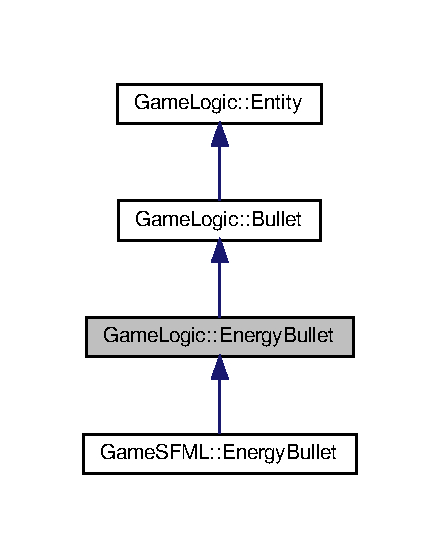
\includegraphics[width=211pt]{classGameLogic_1_1EnergyBullet__inherit__graph}
\end{center}
\end{figure}


Collaboration diagram for Game\+Logic\+:\+:Energy\+Bullet\+:
\nopagebreak
\begin{figure}[H]
\begin{center}
\leavevmode
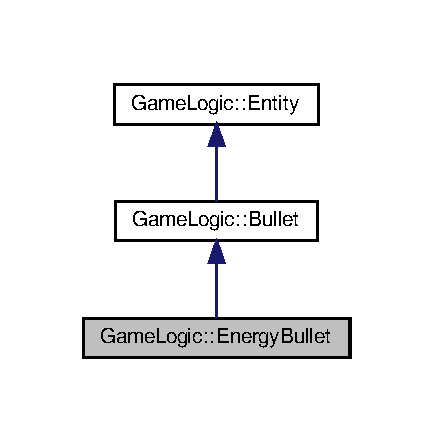
\includegraphics[width=208pt]{classGameLogic_1_1EnergyBullet__coll__graph}
\end{center}
\end{figure}
\subsection*{Public Member Functions}
\begin{DoxyCompactItemize}
\item 
\hyperlink{classGameLogic_1_1EnergyBullet_a0186eb8346b81f63fb1c0e8312cbb583}{Energy\+Bullet} (const pair$<$ int, int $>$ \&position, double width, double height)
\begin{DoxyCompactList}\small\item\em Constructor for the Game Logic version of \hyperlink{classGameLogic_1_1EnergyBullet}{Energy\+Bullet}. \end{DoxyCompactList}\item 
void \hyperlink{classGameLogic_1_1EnergyBullet_a5eafebaf5fccf0a3bf3375def4ff32d2}{handle\+Collision} (const shared\+\_\+ptr$<$ \hyperlink{classGameLogic_1_1Entity}{Entity} $>$ \&other\+Entity) override
\begin{DoxyCompactList}\small\item\em Handles what happens if the bullet collides with another entity. \end{DoxyCompactList}\end{DoxyCompactItemize}
\subsection*{Additional Inherited Members}


\subsection{Detailed Description}
Class to represent the bullets shot by the player. 

\subsection{Constructor \& Destructor Documentation}
\mbox{\Hypertarget{classGameLogic_1_1EnergyBullet_a0186eb8346b81f63fb1c0e8312cbb583}\label{classGameLogic_1_1EnergyBullet_a0186eb8346b81f63fb1c0e8312cbb583}} 
\index{Game\+Logic\+::\+Energy\+Bullet@{Game\+Logic\+::\+Energy\+Bullet}!Energy\+Bullet@{Energy\+Bullet}}
\index{Energy\+Bullet@{Energy\+Bullet}!Game\+Logic\+::\+Energy\+Bullet@{Game\+Logic\+::\+Energy\+Bullet}}
\subsubsection{\texorpdfstring{Energy\+Bullet()}{EnergyBullet()}}
{\footnotesize\ttfamily Game\+Logic\+::\+Energy\+Bullet\+::\+Energy\+Bullet (\begin{DoxyParamCaption}\item[{const pair$<$ int, int $>$ \&}]{position,  }\item[{double}]{width,  }\item[{double}]{height }\end{DoxyParamCaption})}

Constructor for the Game Logic version of \hyperlink{classGameLogic_1_1EnergyBullet}{Energy\+Bullet}. 
\begin{DoxyParams}{Parameters}
{\em position} & the starting position of the bullet \\
\hline
{\em width} & the width of the bullet. \\
\hline
{\em height} & the height of the bullet. \\
\hline
\end{DoxyParams}


\subsection{Member Function Documentation}
\mbox{\Hypertarget{classGameLogic_1_1EnergyBullet_a5eafebaf5fccf0a3bf3375def4ff32d2}\label{classGameLogic_1_1EnergyBullet_a5eafebaf5fccf0a3bf3375def4ff32d2}} 
\index{Game\+Logic\+::\+Energy\+Bullet@{Game\+Logic\+::\+Energy\+Bullet}!handle\+Collision@{handle\+Collision}}
\index{handle\+Collision@{handle\+Collision}!Game\+Logic\+::\+Energy\+Bullet@{Game\+Logic\+::\+Energy\+Bullet}}
\subsubsection{\texorpdfstring{handle\+Collision()}{handleCollision()}}
{\footnotesize\ttfamily void Game\+Logic\+::\+Energy\+Bullet\+::handle\+Collision (\begin{DoxyParamCaption}\item[{const shared\+\_\+ptr$<$ \hyperlink{classGameLogic_1_1Entity}{Entity} $>$ \&}]{other\+Entity }\end{DoxyParamCaption})\hspace{0.3cm}{\ttfamily [override]}, {\ttfamily [virtual]}}

Handles what happens if the bullet collides with another entity. 
\begin{DoxyParams}{Parameters}
{\em other\+Entity} & the other entity it collides with. \\
\hline
\end{DoxyParams}


Reimplemented from \hyperlink{classGameLogic_1_1Entity_af3461a4c6321b1af250821d7a1329ba7}{Game\+Logic\+::\+Entity}.



The documentation for this class was generated from the following files\+:\begin{DoxyCompactItemize}
\item 
Game\+Logic/\+Include/\+Game\+Logic/Energy\+Bullet.\+h\item 
Game\+Logic/src/Energy\+Bullet.\+cpp\end{DoxyCompactItemize}

\hypertarget{classGameSFML_1_1EnergyBullet}{}\section{Game\+S\+F\+ML\+:\+:Energy\+Bullet Class Reference}
\label{classGameSFML_1_1EnergyBullet}\index{Game\+S\+F\+M\+L\+::\+Energy\+Bullet@{Game\+S\+F\+M\+L\+::\+Energy\+Bullet}}


Inheritance diagram for Game\+S\+F\+ML\+:\+:Energy\+Bullet\+:
\nopagebreak
\begin{figure}[H]
\begin{center}
\leavevmode
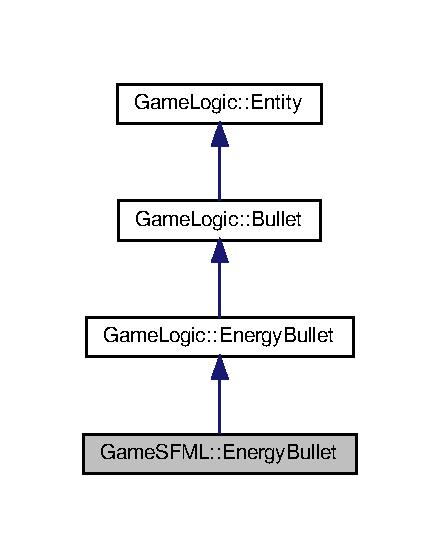
\includegraphics[width=211pt]{classGameSFML_1_1EnergyBullet__inherit__graph}
\end{center}
\end{figure}


Collaboration diagram for Game\+S\+F\+ML\+:\+:Energy\+Bullet\+:
\nopagebreak
\begin{figure}[H]
\begin{center}
\leavevmode
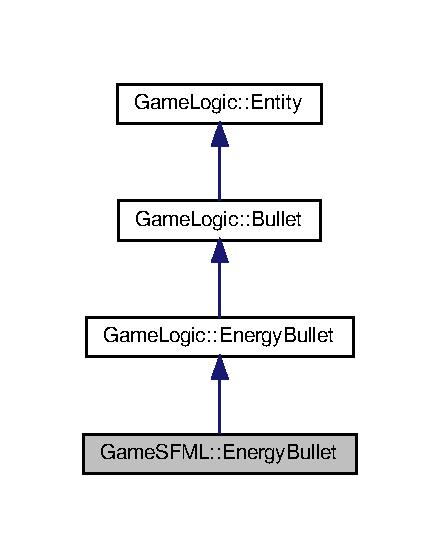
\includegraphics[width=211pt]{classGameSFML_1_1EnergyBullet__coll__graph}
\end{center}
\end{figure}
\subsection*{Public Member Functions}
\begin{DoxyCompactItemize}
\item 
\hyperlink{classGameSFML_1_1EnergyBullet_a4f0effa64f046e9b71a28a4db78dbce7}{Energy\+Bullet} (const pair$<$ int, int $>$ \&position, double width, double height, const string \&file\+Name, const window\+\_\+ptr \&window)
\begin{DoxyCompactList}\small\item\em Constructor of the S\+F\+ML \hyperlink{classGameSFML_1_1BasicEnemyBullet}{Basic\+Enemy\+Bullet}. \end{DoxyCompactList}\item 
void \hyperlink{classGameSFML_1_1EnergyBullet_a41dd2b4aa08fb8af139870c29fa94c00}{draw} () override
\begin{DoxyCompactList}\small\item\em Updates the sprite and draws it to the window. \end{DoxyCompactList}\item 
void \hyperlink{classGameSFML_1_1EnergyBullet_a692e9ae4d828deec21e832986a734ca7}{update\+Sprite} ()
\begin{DoxyCompactList}\small\item\em Updates the sprite to the current position. \end{DoxyCompactList}\end{DoxyCompactItemize}
\subsection*{Additional Inherited Members}


\subsection{Constructor \& Destructor Documentation}
\mbox{\Hypertarget{classGameSFML_1_1EnergyBullet_a4f0effa64f046e9b71a28a4db78dbce7}\label{classGameSFML_1_1EnergyBullet_a4f0effa64f046e9b71a28a4db78dbce7}} 
\index{Game\+S\+F\+M\+L\+::\+Energy\+Bullet@{Game\+S\+F\+M\+L\+::\+Energy\+Bullet}!Energy\+Bullet@{Energy\+Bullet}}
\index{Energy\+Bullet@{Energy\+Bullet}!Game\+S\+F\+M\+L\+::\+Energy\+Bullet@{Game\+S\+F\+M\+L\+::\+Energy\+Bullet}}
\subsubsection{\texorpdfstring{Energy\+Bullet()}{EnergyBullet()}}
{\footnotesize\ttfamily Game\+S\+F\+M\+L\+::\+Energy\+Bullet\+::\+Energy\+Bullet (\begin{DoxyParamCaption}\item[{const pair$<$ int, int $>$ \&}]{position,  }\item[{double}]{width,  }\item[{double}]{height,  }\item[{const string \&}]{file\+Name,  }\item[{const window\+\_\+ptr \&}]{window }\end{DoxyParamCaption})}

Constructor of the S\+F\+ML \hyperlink{classGameSFML_1_1EnergyBullet}{Energy\+Bullet}. 
\begin{DoxyParams}{Parameters}
{\em position} & Position in the grid of the bullet \\
\hline
{\em width} & width of the bullet \\
\hline
{\em height} & height of the bullet \\
\hline
{\em file\+Name} & name of the file of the sprite of the bullet \\
\hline
{\em window} & current game window \\
\hline
\end{DoxyParams}


\subsection{Member Function Documentation}
\mbox{\Hypertarget{classGameSFML_1_1EnergyBullet_a41dd2b4aa08fb8af139870c29fa94c00}\label{classGameSFML_1_1EnergyBullet_a41dd2b4aa08fb8af139870c29fa94c00}} 
\index{Game\+S\+F\+M\+L\+::\+Energy\+Bullet@{Game\+S\+F\+M\+L\+::\+Energy\+Bullet}!draw@{draw}}
\index{draw@{draw}!Game\+S\+F\+M\+L\+::\+Energy\+Bullet@{Game\+S\+F\+M\+L\+::\+Energy\+Bullet}}
\subsubsection{\texorpdfstring{draw()}{draw()}}
{\footnotesize\ttfamily void Game\+S\+F\+M\+L\+::\+Energy\+Bullet\+::draw (\begin{DoxyParamCaption}{ }\end{DoxyParamCaption})\hspace{0.3cm}{\ttfamily [override]}, {\ttfamily [virtual]}}

Updates the sprite and draws it to the window. 

Implements \hyperlink{classGameLogic_1_1Entity_adf23a7036cb99dfc6e33434018131da4}{Game\+Logic\+::\+Entity}.

\mbox{\Hypertarget{classGameSFML_1_1EnergyBullet_a692e9ae4d828deec21e832986a734ca7}\label{classGameSFML_1_1EnergyBullet_a692e9ae4d828deec21e832986a734ca7}} 
\index{Game\+S\+F\+M\+L\+::\+Energy\+Bullet@{Game\+S\+F\+M\+L\+::\+Energy\+Bullet}!update\+Sprite@{update\+Sprite}}
\index{update\+Sprite@{update\+Sprite}!Game\+S\+F\+M\+L\+::\+Energy\+Bullet@{Game\+S\+F\+M\+L\+::\+Energy\+Bullet}}
\subsubsection{\texorpdfstring{update\+Sprite()}{updateSprite()}}
{\footnotesize\ttfamily void Game\+S\+F\+M\+L\+::\+Energy\+Bullet\+::update\+Sprite (\begin{DoxyParamCaption}{ }\end{DoxyParamCaption})}

Updates the sprite to the current position. 

The documentation for this class was generated from the following files\+:\begin{DoxyCompactItemize}
\item 
S\+F\+M\+L/\+Include/Energy\+Bullet.\+h\item 
S\+F\+M\+L/src/Energy\+Bullet.\+cpp\end{DoxyCompactItemize}

\hypertarget{classGameLogic_1_1EnergyCannon}{}\section{Game\+Logic\+:\+:Energy\+Cannon Class Reference}
\label{classGameLogic_1_1EnergyCannon}\index{Game\+Logic\+::\+Energy\+Cannon@{Game\+Logic\+::\+Energy\+Cannon}}


Class that represents the cannons used for shooting down enemies.  




{\ttfamily \#include $<$Energy\+Cannon.\+h$>$}



Inheritance diagram for Game\+Logic\+:\+:Energy\+Cannon\+:\nopagebreak
\begin{figure}[H]
\begin{center}
\leavevmode
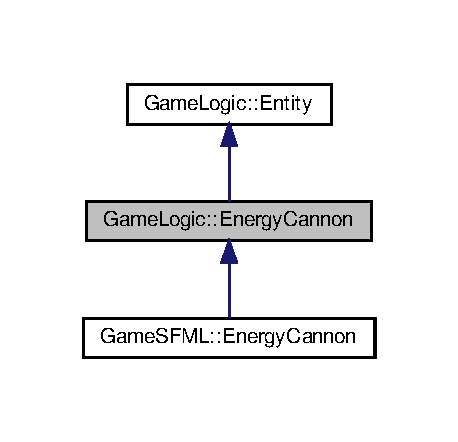
\includegraphics[width=220pt]{classGameLogic_1_1EnergyCannon__inherit__graph}
\end{center}
\end{figure}


Collaboration diagram for Game\+Logic\+:\+:Energy\+Cannon\+:\nopagebreak
\begin{figure}[H]
\begin{center}
\leavevmode
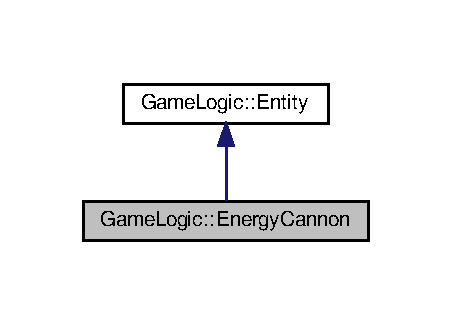
\includegraphics[width=217pt]{classGameLogic_1_1EnergyCannon__coll__graph}
\end{center}
\end{figure}
\subsection*{Public Member Functions}
\begin{DoxyCompactItemize}
\item 
\hyperlink{classGameLogic_1_1EnergyCannon_aa2d03f1f31cc13454d958a0f81c241bc}{Energy\+Cannon} (const pair$<$ int, int $>$ \&position, double width, double height)
\begin{DoxyCompactList}\small\item\em Constructor for the energy cannons. \end{DoxyCompactList}\item 
bool \hyperlink{classGameLogic_1_1EnergyCannon_a8028f1d9d52870997eae9335e9c494f5}{shoot} ()
\begin{DoxyCompactList}\small\item\em Shoots the cannon. \end{DoxyCompactList}\item 
bool \hyperlink{classGameLogic_1_1EnergyCannon_a584235c8d7a30c927338d753ed705968}{auto\+Reload} ()
\begin{DoxyCompactList}\small\item\em Reloads the cannon if not used for some time. \end{DoxyCompactList}\item 
bool \hyperlink{classGameLogic_1_1EnergyCannon_aa83309544f619024d575b88745260d8e}{reload} ()
\begin{DoxyCompactList}\small\item\em Reload the cannon. \end{DoxyCompactList}\item 
void \hyperlink{classGameLogic_1_1EnergyCannon_a29274434c4a4f12bbf829eb4f6fa2559}{lower\+Delay} ()
\begin{DoxyCompactList}\small\item\em Lowers the shot\+Delay by 1. \end{DoxyCompactList}\item 
void \hyperlink{classGameLogic_1_1EnergyCannon_a1499b7d8e1df720b314a263f61e69e7d}{increase\+Time\+Not\+Used} ()
\begin{DoxyCompactList}\small\item\em Increases the time\+Not\+Used counter by 1. \end{DoxyCompactList}\end{DoxyCompactItemize}
\subsection*{Protected Attributes}
\begin{DoxyCompactItemize}
\item 
\mbox{\Hypertarget{classGameLogic_1_1EnergyCannon_ac08c44df7f23b72b1b99313015026f39}\label{classGameLogic_1_1EnergyCannon_ac08c44df7f23b72b1b99313015026f39}} 
int {\bfseries remaining\+Bullets} = 8
\end{DoxyCompactItemize}
\subsection*{Additional Inherited Members}


\subsection{Detailed Description}
Class that represents the cannons used for shooting down enemies. 

\subsection{Constructor \& Destructor Documentation}
\mbox{\Hypertarget{classGameLogic_1_1EnergyCannon_aa2d03f1f31cc13454d958a0f81c241bc}\label{classGameLogic_1_1EnergyCannon_aa2d03f1f31cc13454d958a0f81c241bc}} 
\index{Game\+Logic\+::\+Energy\+Cannon@{Game\+Logic\+::\+Energy\+Cannon}!Energy\+Cannon@{Energy\+Cannon}}
\index{Energy\+Cannon@{Energy\+Cannon}!Game\+Logic\+::\+Energy\+Cannon@{Game\+Logic\+::\+Energy\+Cannon}}
\subsubsection{\texorpdfstring{Energy\+Cannon()}{EnergyCannon()}}
{\footnotesize\ttfamily Game\+Logic\+::\+Energy\+Cannon\+::\+Energy\+Cannon (\begin{DoxyParamCaption}\item[{const pair$<$ int, int $>$ \&}]{position,  }\item[{double}]{width,  }\item[{double}]{height }\end{DoxyParamCaption})}

Constructor for the energy cannons. 
\begin{DoxyParams}{Parameters}
{\em position} & The position in the grid of the cannon. \\
\hline
{\em width} & The width of the cannon. \\
\hline
{\em height} & The height of the cannon. \\
\hline
\end{DoxyParams}


\subsection{Member Function Documentation}
\mbox{\Hypertarget{classGameLogic_1_1EnergyCannon_a584235c8d7a30c927338d753ed705968}\label{classGameLogic_1_1EnergyCannon_a584235c8d7a30c927338d753ed705968}} 
\index{Game\+Logic\+::\+Energy\+Cannon@{Game\+Logic\+::\+Energy\+Cannon}!auto\+Reload@{auto\+Reload}}
\index{auto\+Reload@{auto\+Reload}!Game\+Logic\+::\+Energy\+Cannon@{Game\+Logic\+::\+Energy\+Cannon}}
\subsubsection{\texorpdfstring{auto\+Reload()}{autoReload()}}
{\footnotesize\ttfamily bool Game\+Logic\+::\+Energy\+Cannon\+::auto\+Reload (\begin{DoxyParamCaption}{ }\end{DoxyParamCaption})}

Reloads the cannon if not used for some time. Returns true if able to reload. \begin{DoxyReturn}{Returns}
True is able to reload. 
\end{DoxyReturn}
\mbox{\Hypertarget{classGameLogic_1_1EnergyCannon_a1499b7d8e1df720b314a263f61e69e7d}\label{classGameLogic_1_1EnergyCannon_a1499b7d8e1df720b314a263f61e69e7d}} 
\index{Game\+Logic\+::\+Energy\+Cannon@{Game\+Logic\+::\+Energy\+Cannon}!increase\+Time\+Not\+Used@{increase\+Time\+Not\+Used}}
\index{increase\+Time\+Not\+Used@{increase\+Time\+Not\+Used}!Game\+Logic\+::\+Energy\+Cannon@{Game\+Logic\+::\+Energy\+Cannon}}
\subsubsection{\texorpdfstring{increase\+Time\+Not\+Used()}{increaseTimeNotUsed()}}
{\footnotesize\ttfamily void Game\+Logic\+::\+Energy\+Cannon\+::increase\+Time\+Not\+Used (\begin{DoxyParamCaption}{ }\end{DoxyParamCaption})}

Increases the time\+Not\+Used counter by 1. \mbox{\Hypertarget{classGameLogic_1_1EnergyCannon_a29274434c4a4f12bbf829eb4f6fa2559}\label{classGameLogic_1_1EnergyCannon_a29274434c4a4f12bbf829eb4f6fa2559}} 
\index{Game\+Logic\+::\+Energy\+Cannon@{Game\+Logic\+::\+Energy\+Cannon}!lower\+Delay@{lower\+Delay}}
\index{lower\+Delay@{lower\+Delay}!Game\+Logic\+::\+Energy\+Cannon@{Game\+Logic\+::\+Energy\+Cannon}}
\subsubsection{\texorpdfstring{lower\+Delay()}{lowerDelay()}}
{\footnotesize\ttfamily void Game\+Logic\+::\+Energy\+Cannon\+::lower\+Delay (\begin{DoxyParamCaption}{ }\end{DoxyParamCaption})}

Lowers the shot\+Delay by 1. \mbox{\Hypertarget{classGameLogic_1_1EnergyCannon_aa83309544f619024d575b88745260d8e}\label{classGameLogic_1_1EnergyCannon_aa83309544f619024d575b88745260d8e}} 
\index{Game\+Logic\+::\+Energy\+Cannon@{Game\+Logic\+::\+Energy\+Cannon}!reload@{reload}}
\index{reload@{reload}!Game\+Logic\+::\+Energy\+Cannon@{Game\+Logic\+::\+Energy\+Cannon}}
\subsubsection{\texorpdfstring{reload()}{reload()}}
{\footnotesize\ttfamily bool Game\+Logic\+::\+Energy\+Cannon\+::reload (\begin{DoxyParamCaption}{ }\end{DoxyParamCaption})}

Reload the cannon. Returns whether the reload was possible or not. \begin{DoxyReturn}{Returns}
True if the reload was possible. 
\end{DoxyReturn}
\mbox{\Hypertarget{classGameLogic_1_1EnergyCannon_a8028f1d9d52870997eae9335e9c494f5}\label{classGameLogic_1_1EnergyCannon_a8028f1d9d52870997eae9335e9c494f5}} 
\index{Game\+Logic\+::\+Energy\+Cannon@{Game\+Logic\+::\+Energy\+Cannon}!shoot@{shoot}}
\index{shoot@{shoot}!Game\+Logic\+::\+Energy\+Cannon@{Game\+Logic\+::\+Energy\+Cannon}}
\subsubsection{\texorpdfstring{shoot()}{shoot()}}
{\footnotesize\ttfamily bool Game\+Logic\+::\+Energy\+Cannon\+::shoot (\begin{DoxyParamCaption}{ }\end{DoxyParamCaption})}

If the cannon has enough bullets it return that is shoots and resets time not used to 0, else it returns false. \begin{DoxyReturn}{Returns}
Whether the cannon shoots or not. 
\end{DoxyReturn}


The documentation for this class was generated from the following files\+:\begin{DoxyCompactItemize}
\item 
Game\+Logic/\+Include/\+Game\+Logic/Energy\+Cannon.\+h\item 
Game\+Logic/src/Energy\+Cannon.\+cpp\end{DoxyCompactItemize}

\hypertarget{classGameSFML_1_1EnergyCannon}{}\section{Game\+S\+F\+ML\+:\+:Energy\+Cannon Class Reference}
\label{classGameSFML_1_1EnergyCannon}\index{Game\+S\+F\+M\+L\+::\+Energy\+Cannon@{Game\+S\+F\+M\+L\+::\+Energy\+Cannon}}


S\+F\+ML version of the \hyperlink{classGameSFML_1_1EnergyCannon}{Energy\+Cannon} class.  




{\ttfamily \#include $<$Energy\+Cannon.\+h$>$}



Inheritance diagram for Game\+S\+F\+ML\+:\+:Energy\+Cannon\+:
\nopagebreak
\begin{figure}[H]
\begin{center}
\leavevmode
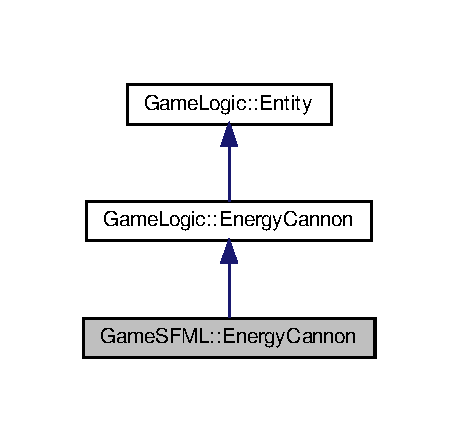
\includegraphics[width=220pt]{classGameSFML_1_1EnergyCannon__inherit__graph}
\end{center}
\end{figure}


Collaboration diagram for Game\+S\+F\+ML\+:\+:Energy\+Cannon\+:
\nopagebreak
\begin{figure}[H]
\begin{center}
\leavevmode
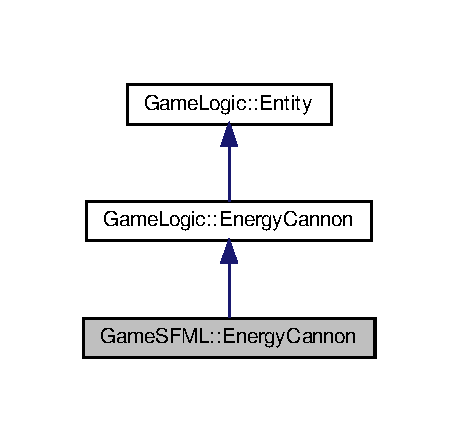
\includegraphics[width=220pt]{classGameSFML_1_1EnergyCannon__coll__graph}
\end{center}
\end{figure}
\subsection*{Public Member Functions}
\begin{DoxyCompactItemize}
\item 
\hyperlink{classGameSFML_1_1EnergyCannon_a456f26d38873ce81105fe14657bcbed3}{Energy\+Cannon} (const pair$<$ int, int $>$ \&position, double width, double height, const string \&file\+Name, const window\+\_\+ptr \&window)
\begin{DoxyCompactList}\small\item\em Constructor of the S\+F\+ML version of \hyperlink{classGameSFML_1_1EnergyCannon}{Energy\+Cannon}. \end{DoxyCompactList}\item 
void \hyperlink{classGameSFML_1_1EnergyCannon_a9c4c44e9ded9422d790c685d5901cb64}{draw} () override
\begin{DoxyCompactList}\small\item\em Updates the sprite and draws it to the window. \end{DoxyCompactList}\item 
void \hyperlink{classGameSFML_1_1EnergyCannon_a2d71ccd7276055f9b5f9e688545d5982}{update\+Sprite} ()
\begin{DoxyCompactList}\small\item\em Updates the sprite to the current position. \end{DoxyCompactList}\end{DoxyCompactItemize}
\subsection*{Additional Inherited Members}


\subsection{Detailed Description}
S\+F\+ML version of the \hyperlink{classGameSFML_1_1EnergyCannon}{Energy\+Cannon} class. 

\subsection{Constructor \& Destructor Documentation}
\mbox{\Hypertarget{classGameSFML_1_1EnergyCannon_a456f26d38873ce81105fe14657bcbed3}\label{classGameSFML_1_1EnergyCannon_a456f26d38873ce81105fe14657bcbed3}} 
\index{Game\+S\+F\+M\+L\+::\+Energy\+Cannon@{Game\+S\+F\+M\+L\+::\+Energy\+Cannon}!Energy\+Cannon@{Energy\+Cannon}}
\index{Energy\+Cannon@{Energy\+Cannon}!Game\+S\+F\+M\+L\+::\+Energy\+Cannon@{Game\+S\+F\+M\+L\+::\+Energy\+Cannon}}
\subsubsection{\texorpdfstring{Energy\+Cannon()}{EnergyCannon()}}
{\footnotesize\ttfamily Game\+S\+F\+M\+L\+::\+Energy\+Cannon\+::\+Energy\+Cannon (\begin{DoxyParamCaption}\item[{const pair$<$ int, int $>$ \&}]{position,  }\item[{double}]{width,  }\item[{double}]{height,  }\item[{const string \&}]{file\+Name,  }\item[{const window\+\_\+ptr \&}]{window }\end{DoxyParamCaption})}

Constructor of the S\+F\+ML version of \hyperlink{classGameSFML_1_1EnergyCannon}{Energy\+Cannon}. 
\begin{DoxyParams}{Parameters}
{\em position} & The position in the grid of the cannon. \\
\hline
{\em width} & The width of the cannon. \\
\hline
{\em height} & The height of the cannon. \\
\hline
{\em file\+Name} & The name of the file that contains the sprite of the cannon. \\
\hline
{\em window} & The current game window \\
\hline
\end{DoxyParams}


\subsection{Member Function Documentation}
\mbox{\Hypertarget{classGameSFML_1_1EnergyCannon_a9c4c44e9ded9422d790c685d5901cb64}\label{classGameSFML_1_1EnergyCannon_a9c4c44e9ded9422d790c685d5901cb64}} 
\index{Game\+S\+F\+M\+L\+::\+Energy\+Cannon@{Game\+S\+F\+M\+L\+::\+Energy\+Cannon}!draw@{draw}}
\index{draw@{draw}!Game\+S\+F\+M\+L\+::\+Energy\+Cannon@{Game\+S\+F\+M\+L\+::\+Energy\+Cannon}}
\subsubsection{\texorpdfstring{draw()}{draw()}}
{\footnotesize\ttfamily void Game\+S\+F\+M\+L\+::\+Energy\+Cannon\+::draw (\begin{DoxyParamCaption}{ }\end{DoxyParamCaption})\hspace{0.3cm}{\ttfamily [override]}, {\ttfamily [virtual]}}

Updates the sprite and draws it to the window. 

Implements \hyperlink{classGameLogic_1_1Entity_adf23a7036cb99dfc6e33434018131da4}{Game\+Logic\+::\+Entity}.

\mbox{\Hypertarget{classGameSFML_1_1EnergyCannon_a2d71ccd7276055f9b5f9e688545d5982}\label{classGameSFML_1_1EnergyCannon_a2d71ccd7276055f9b5f9e688545d5982}} 
\index{Game\+S\+F\+M\+L\+::\+Energy\+Cannon@{Game\+S\+F\+M\+L\+::\+Energy\+Cannon}!update\+Sprite@{update\+Sprite}}
\index{update\+Sprite@{update\+Sprite}!Game\+S\+F\+M\+L\+::\+Energy\+Cannon@{Game\+S\+F\+M\+L\+::\+Energy\+Cannon}}
\subsubsection{\texorpdfstring{update\+Sprite()}{updateSprite()}}
{\footnotesize\ttfamily void Game\+S\+F\+M\+L\+::\+Energy\+Cannon\+::update\+Sprite (\begin{DoxyParamCaption}{ }\end{DoxyParamCaption})}

Updates the sprite to the current position. 

The documentation for this class was generated from the following files\+:\begin{DoxyCompactItemize}
\item 
S\+F\+M\+L/\+Include/Energy\+Cannon.\+h\item 
S\+F\+M\+L/src/Energy\+Cannon.\+cpp\end{DoxyCompactItemize}

\hypertarget{classGameLogic_1_1Entity}{}\section{Game\+Logic\+:\+:Entity Class Reference}
\label{classGameLogic_1_1Entity}\index{Game\+Logic\+::\+Entity@{Game\+Logic\+::\+Entity}}


Base \hyperlink{classGameLogic_1_1Entity}{Entity} class Base entity class, most classes will be derived from this.  




{\ttfamily \#include $<$Entity.\+h$>$}



Inheritance diagram for Game\+Logic\+:\+:Entity\+:
\nopagebreak
\begin{figure}[H]
\begin{center}
\leavevmode
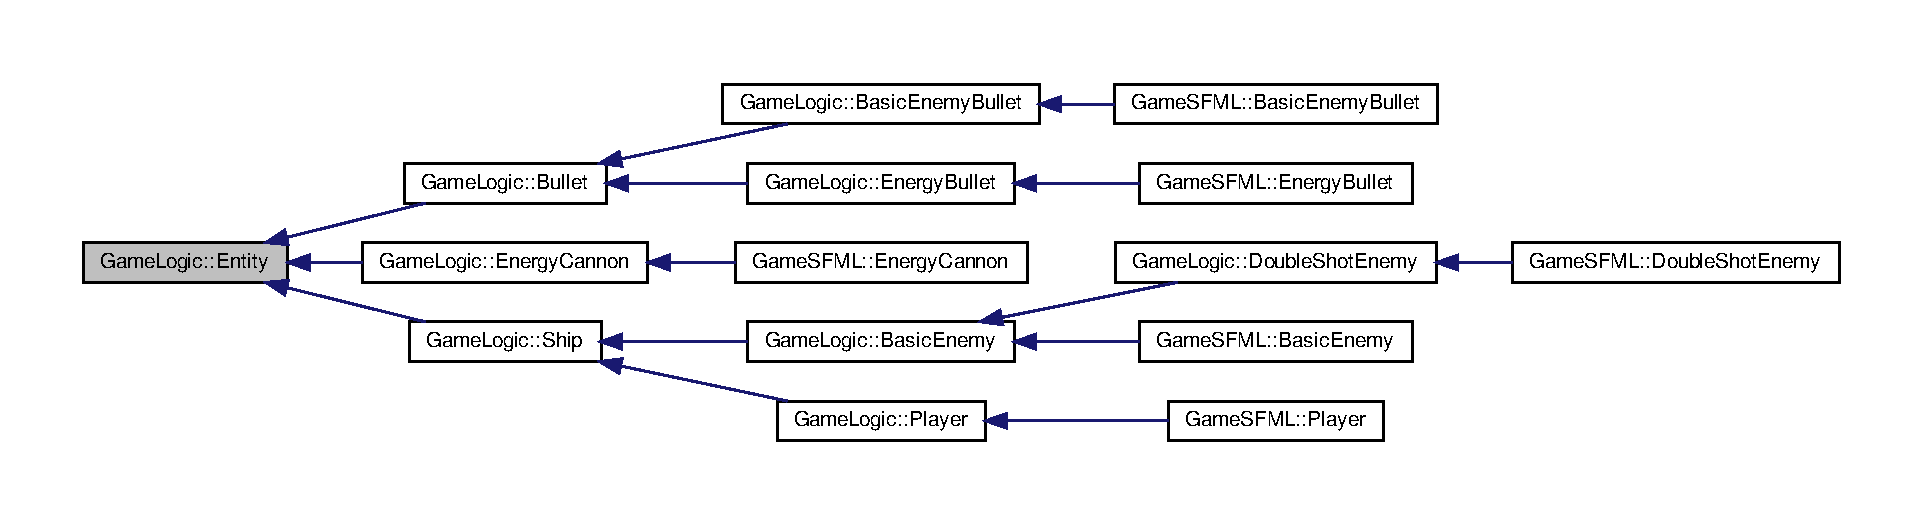
\includegraphics[width=350pt]{classGameLogic_1_1Entity__inherit__graph}
\end{center}
\end{figure}
\subsection*{Public Member Functions}
\begin{DoxyCompactItemize}
\item 
\hyperlink{classGameLogic_1_1Entity_ace7cd95750149d125c00bb7786527cbf}{Entity} (const pair$<$ int, int $>$ \&position, double width, double height)
\begin{DoxyCompactList}\small\item\em Constructor of \hyperlink{classGameLogic_1_1Entity}{Entity} Constructor of \hyperlink{classGameLogic_1_1Entity}{Entity}. \end{DoxyCompactList}\item 
int \hyperlink{classGameLogic_1_1Entity_a1d7c4fa1af58df883ae751c4e536c25d}{getX} ()
\begin{DoxyCompactList}\small\item\em Function to return the x coordinate Function to get the x position in the grid. \end{DoxyCompactList}\item 
int \hyperlink{classGameLogic_1_1Entity_a24a56a7da02136fd662b72b04fcf6c30}{getY} ()
\begin{DoxyCompactList}\small\item\em Function to return the y coordinate Function to get the y position in the grid. \end{DoxyCompactList}\item 
string \hyperlink{classGameLogic_1_1Entity_a8bdd4210279142027ba149483b89ff01}{get\+Type} ()
\begin{DoxyCompactList}\small\item\em Function that returns the type Function that returns the type of \hyperlink{classGameLogic_1_1Entity}{Entity} (e.\+g. \end{DoxyCompactList}\item 
void \hyperlink{classGameLogic_1_1Entity_a570383f8bb12fc3185d136289f2149c8}{setX} (int x)
\begin{DoxyCompactList}\small\item\em Function to set the x coordinate Function that sets the x coordinate in the grid. \end{DoxyCompactList}\item 
void \hyperlink{classGameLogic_1_1Entity_a246c3603f576c080df17978b483ada45}{setY} (int y)
\begin{DoxyCompactList}\small\item\em Function to set the y coordinate Function that sets the y coordinate in the grid. \end{DoxyCompactList}\item 
void \hyperlink{classGameLogic_1_1Entity_ae0f16e2b996a2654851e757dfa255ba9}{set\+Speed} (double speed)
\begin{DoxyCompactList}\small\item\em Function that sets the entity\textquotesingle{}s speed Function that sets the speed of the entity. \end{DoxyCompactList}\item 
double \hyperlink{classGameLogic_1_1Entity_a7c0d8853692bccc978847b658d45fb5e}{get\+Speed} ()
\begin{DoxyCompactList}\small\item\em Function that gets the entity\textquotesingle{}s speed Function that returns the speed of the entity. \end{DoxyCompactList}\item 
double \hyperlink{classGameLogic_1_1Entity_a770b837c07c91f3fa72c755d6d77d153}{get\+MovingX} () const
\begin{DoxyCompactList}\small\item\em Function to return the moving x coordinate Function to get the x position used for fluid movement on screen. \end{DoxyCompactList}\item 
void \hyperlink{classGameLogic_1_1Entity_a0610847bac56b7ec45dff937f20c048b}{add\+MovingX} (double addedX)
\begin{DoxyCompactList}\small\item\em Function to add to the moving x coordinate Function to add to the x position used for fluid movement on screen. \end{DoxyCompactList}\item 
double \hyperlink{classGameLogic_1_1Entity_a5e10708660f91ce9a225c08ebbecf7fd}{get\+MovingY} () const
\begin{DoxyCompactList}\small\item\em Function to return the moving y coordinate Function to get the y position used for fluid movement on screen. \end{DoxyCompactList}\item 
void \hyperlink{classGameLogic_1_1Entity_ad46302e582b23b71e250f15c47f59ee0}{add\+MovingY} (double addedY)
\begin{DoxyCompactList}\small\item\em Function to add to the moving y coordinate Function to add to the y position used for fluid movement on screen. \end{DoxyCompactList}\item 
virtual void \hyperlink{classGameLogic_1_1Entity_adf23a7036cb99dfc6e33434018131da4}{draw} ()=0
\begin{DoxyCompactList}\small\item\em Virtual draw function in \hyperlink{classGameLogic_1_1Entity}{Entity}. \end{DoxyCompactList}\item 
bool \hyperlink{classGameLogic_1_1Entity_ac1521f845aac18a02bc8a2434579919e}{check\+If\+Removable} ()
\begin{DoxyCompactList}\small\item\em Checks if the entity is removable. \end{DoxyCompactList}\item 
void \hyperlink{classGameLogic_1_1Entity_a5bfae36adfedd3652d8dd8a807184c5f}{remove} ()
\begin{DoxyCompactList}\small\item\em Makes the entity ready to be removed. \end{DoxyCompactList}\item 
double \hyperlink{classGameLogic_1_1Entity_a9a7be1c6095ef036eb91b962cd289dc3}{get\+Width} () const
\begin{DoxyCompactList}\small\item\em Gets the width of the entity. \end{DoxyCompactList}\item 
double \hyperlink{classGameLogic_1_1Entity_a8d66c2c0153168c3ad9d345327f2c866}{get\+Height} () const
\begin{DoxyCompactList}\small\item\em Gets the height of the entity. \end{DoxyCompactList}\item 
virtual void \hyperlink{classGameLogic_1_1Entity_af3461a4c6321b1af250821d7a1329ba7}{handle\+Collision} (const shared\+\_\+ptr$<$ \hyperlink{classGameLogic_1_1Entity}{Entity} $>$ \&other\+Entity)
\begin{DoxyCompactList}\small\item\em Virtual function for handling collision. \end{DoxyCompactList}\end{DoxyCompactItemize}
\subsection*{Protected Member Functions}
\begin{DoxyCompactItemize}
\item 
void \hyperlink{classGameLogic_1_1Entity_a5333b148dd17e31aafd6e115e0b3b43d}{set\+Type} (string type)
\begin{DoxyCompactList}\small\item\em Funtion to set the type of the \hyperlink{classGameLogic_1_1Entity}{Entity} Function to set the type of the entity. \end{DoxyCompactList}\end{DoxyCompactItemize}


\subsection{Constructor \& Destructor Documentation}
\mbox{\Hypertarget{classGameLogic_1_1Entity_ace7cd95750149d125c00bb7786527cbf}\label{classGameLogic_1_1Entity_ace7cd95750149d125c00bb7786527cbf}} 
\index{Game\+Logic\+::\+Entity@{Game\+Logic\+::\+Entity}!Entity@{Entity}}
\index{Entity@{Entity}!Game\+Logic\+::\+Entity@{Game\+Logic\+::\+Entity}}
\subsubsection{\texorpdfstring{Entity()}{Entity()}}
{\footnotesize\ttfamily Game\+Logic\+::\+Entity\+::\+Entity (\begin{DoxyParamCaption}\item[{const pair$<$ int, int $>$ \&}]{position,  }\item[{double}]{width,  }\item[{double}]{height }\end{DoxyParamCaption})}


\begin{DoxyParams}{Parameters}
{\em position} & The position of the entity in the grid \\
\hline
{\em width} & The width of the entity \\
\hline
{\em height} & The height of the entity \\
\hline
\end{DoxyParams}


\subsection{Member Function Documentation}
\mbox{\Hypertarget{classGameLogic_1_1Entity_a0610847bac56b7ec45dff937f20c048b}\label{classGameLogic_1_1Entity_a0610847bac56b7ec45dff937f20c048b}} 
\index{Game\+Logic\+::\+Entity@{Game\+Logic\+::\+Entity}!add\+MovingX@{add\+MovingX}}
\index{add\+MovingX@{add\+MovingX}!Game\+Logic\+::\+Entity@{Game\+Logic\+::\+Entity}}
\subsubsection{\texorpdfstring{add\+Moving\+X()}{addMovingX()}}
{\footnotesize\ttfamily void Game\+Logic\+::\+Entity\+::add\+MovingX (\begin{DoxyParamCaption}\item[{double}]{addedX }\end{DoxyParamCaption})}


\begin{DoxyParams}{Parameters}
{\em movingX} & Double value to be added (or subtracted using a negative value) to the existing moving x value \\
\hline
\end{DoxyParams}
\mbox{\Hypertarget{classGameLogic_1_1Entity_ad46302e582b23b71e250f15c47f59ee0}\label{classGameLogic_1_1Entity_ad46302e582b23b71e250f15c47f59ee0}} 
\index{Game\+Logic\+::\+Entity@{Game\+Logic\+::\+Entity}!add\+MovingY@{add\+MovingY}}
\index{add\+MovingY@{add\+MovingY}!Game\+Logic\+::\+Entity@{Game\+Logic\+::\+Entity}}
\subsubsection{\texorpdfstring{add\+Moving\+Y()}{addMovingY()}}
{\footnotesize\ttfamily void Game\+Logic\+::\+Entity\+::add\+MovingY (\begin{DoxyParamCaption}\item[{double}]{addedY }\end{DoxyParamCaption})}


\begin{DoxyParams}{Parameters}
{\em movingX} & Double value to be added (or subtracted using a negative value) to the existing moving y value \\
\hline
\end{DoxyParams}
\mbox{\Hypertarget{classGameLogic_1_1Entity_ac1521f845aac18a02bc8a2434579919e}\label{classGameLogic_1_1Entity_ac1521f845aac18a02bc8a2434579919e}} 
\index{Game\+Logic\+::\+Entity@{Game\+Logic\+::\+Entity}!check\+If\+Removable@{check\+If\+Removable}}
\index{check\+If\+Removable@{check\+If\+Removable}!Game\+Logic\+::\+Entity@{Game\+Logic\+::\+Entity}}
\subsubsection{\texorpdfstring{check\+If\+Removable()}{checkIfRemovable()}}
{\footnotesize\ttfamily bool Game\+Logic\+::\+Entity\+::check\+If\+Removable (\begin{DoxyParamCaption}{ }\end{DoxyParamCaption})}

Checks the value of the removable variable. \begin{DoxyReturn}{Returns}
the value of the removable variable. 
\end{DoxyReturn}
\mbox{\Hypertarget{classGameLogic_1_1Entity_adf23a7036cb99dfc6e33434018131da4}\label{classGameLogic_1_1Entity_adf23a7036cb99dfc6e33434018131da4}} 
\index{Game\+Logic\+::\+Entity@{Game\+Logic\+::\+Entity}!draw@{draw}}
\index{draw@{draw}!Game\+Logic\+::\+Entity@{Game\+Logic\+::\+Entity}}
\subsubsection{\texorpdfstring{draw()}{draw()}}
{\footnotesize\ttfamily void Game\+Logic\+::\+Entity\+::draw (\begin{DoxyParamCaption}{ }\end{DoxyParamCaption})\hspace{0.3cm}{\ttfamily [pure virtual]}}

Virtual draw function in \hyperlink{classGameLogic_1_1Entity}{Entity}. Virtual function 

Implemented in \hyperlink{classGameSFML_1_1BasicEnemy_a1062ddf1321edb7d069b68b396615626}{Game\+S\+F\+M\+L\+::\+Basic\+Enemy}, \hyperlink{classGameSFML_1_1Player_ac694755fafaffdf9432415452c7b9b5b}{Game\+S\+F\+M\+L\+::\+Player}, \hyperlink{classGameSFML_1_1BasicEnemyBullet_af970b7b86c5a21963daac86822a064a2}{Game\+S\+F\+M\+L\+::\+Basic\+Enemy\+Bullet}, \hyperlink{classGameSFML_1_1EnergyCannon_a9c4c44e9ded9422d790c685d5901cb64}{Game\+S\+F\+M\+L\+::\+Energy\+Cannon}, \hyperlink{classGameSFML_1_1EnergyBullet_a41dd2b4aa08fb8af139870c29fa94c00}{Game\+S\+F\+M\+L\+::\+Energy\+Bullet}, and \hyperlink{classGameSFML_1_1DoubleShotEnemy_a3d30aebbab50ad019207d6ba91ab0b5f}{Game\+S\+F\+M\+L\+::\+Double\+Shot\+Enemy}.

\mbox{\Hypertarget{classGameLogic_1_1Entity_a8d66c2c0153168c3ad9d345327f2c866}\label{classGameLogic_1_1Entity_a8d66c2c0153168c3ad9d345327f2c866}} 
\index{Game\+Logic\+::\+Entity@{Game\+Logic\+::\+Entity}!get\+Height@{get\+Height}}
\index{get\+Height@{get\+Height}!Game\+Logic\+::\+Entity@{Game\+Logic\+::\+Entity}}
\subsubsection{\texorpdfstring{get\+Height()}{getHeight()}}
{\footnotesize\ttfamily double Game\+Logic\+::\+Entity\+::get\+Height (\begin{DoxyParamCaption}{ }\end{DoxyParamCaption}) const}

Gets the height of the entity. \begin{DoxyReturn}{Returns}
The height of the entity. 
\end{DoxyReturn}
\mbox{\Hypertarget{classGameLogic_1_1Entity_a770b837c07c91f3fa72c755d6d77d153}\label{classGameLogic_1_1Entity_a770b837c07c91f3fa72c755d6d77d153}} 
\index{Game\+Logic\+::\+Entity@{Game\+Logic\+::\+Entity}!get\+MovingX@{get\+MovingX}}
\index{get\+MovingX@{get\+MovingX}!Game\+Logic\+::\+Entity@{Game\+Logic\+::\+Entity}}
\subsubsection{\texorpdfstring{get\+Moving\+X()}{getMovingX()}}
{\footnotesize\ttfamily double Game\+Logic\+::\+Entity\+::get\+MovingX (\begin{DoxyParamCaption}{ }\end{DoxyParamCaption}) const}

\begin{DoxyReturn}{Returns}
Integer value of the moving x coordinate of the entity 
\end{DoxyReturn}
\mbox{\Hypertarget{classGameLogic_1_1Entity_a5e10708660f91ce9a225c08ebbecf7fd}\label{classGameLogic_1_1Entity_a5e10708660f91ce9a225c08ebbecf7fd}} 
\index{Game\+Logic\+::\+Entity@{Game\+Logic\+::\+Entity}!get\+MovingY@{get\+MovingY}}
\index{get\+MovingY@{get\+MovingY}!Game\+Logic\+::\+Entity@{Game\+Logic\+::\+Entity}}
\subsubsection{\texorpdfstring{get\+Moving\+Y()}{getMovingY()}}
{\footnotesize\ttfamily double Game\+Logic\+::\+Entity\+::get\+MovingY (\begin{DoxyParamCaption}{ }\end{DoxyParamCaption}) const}

\begin{DoxyReturn}{Returns}
Integer value of the moving y coordinate of the entity 
\end{DoxyReturn}
\mbox{\Hypertarget{classGameLogic_1_1Entity_a7c0d8853692bccc978847b658d45fb5e}\label{classGameLogic_1_1Entity_a7c0d8853692bccc978847b658d45fb5e}} 
\index{Game\+Logic\+::\+Entity@{Game\+Logic\+::\+Entity}!get\+Speed@{get\+Speed}}
\index{get\+Speed@{get\+Speed}!Game\+Logic\+::\+Entity@{Game\+Logic\+::\+Entity}}
\subsubsection{\texorpdfstring{get\+Speed()}{getSpeed()}}
{\footnotesize\ttfamily double Game\+Logic\+::\+Entity\+::get\+Speed (\begin{DoxyParamCaption}{ }\end{DoxyParamCaption})}

\begin{DoxyReturn}{Returns}
Double value of the speed of the entity 
\end{DoxyReturn}
\mbox{\Hypertarget{classGameLogic_1_1Entity_a8bdd4210279142027ba149483b89ff01}\label{classGameLogic_1_1Entity_a8bdd4210279142027ba149483b89ff01}} 
\index{Game\+Logic\+::\+Entity@{Game\+Logic\+::\+Entity}!get\+Type@{get\+Type}}
\index{get\+Type@{get\+Type}!Game\+Logic\+::\+Entity@{Game\+Logic\+::\+Entity}}
\subsubsection{\texorpdfstring{get\+Type()}{getType()}}
{\footnotesize\ttfamily string Game\+Logic\+::\+Entity\+::get\+Type (\begin{DoxyParamCaption}{ }\end{DoxyParamCaption})}

\hyperlink{classGameLogic_1_1Player}{Player}) \begin{DoxyReturn}{Returns}
The type of entity 
\end{DoxyReturn}
\mbox{\Hypertarget{classGameLogic_1_1Entity_a9a7be1c6095ef036eb91b962cd289dc3}\label{classGameLogic_1_1Entity_a9a7be1c6095ef036eb91b962cd289dc3}} 
\index{Game\+Logic\+::\+Entity@{Game\+Logic\+::\+Entity}!get\+Width@{get\+Width}}
\index{get\+Width@{get\+Width}!Game\+Logic\+::\+Entity@{Game\+Logic\+::\+Entity}}
\subsubsection{\texorpdfstring{get\+Width()}{getWidth()}}
{\footnotesize\ttfamily double Game\+Logic\+::\+Entity\+::get\+Width (\begin{DoxyParamCaption}{ }\end{DoxyParamCaption}) const}

Gets the width of the entity. \begin{DoxyReturn}{Returns}
The width of the entity. 
\end{DoxyReturn}
\mbox{\Hypertarget{classGameLogic_1_1Entity_a1d7c4fa1af58df883ae751c4e536c25d}\label{classGameLogic_1_1Entity_a1d7c4fa1af58df883ae751c4e536c25d}} 
\index{Game\+Logic\+::\+Entity@{Game\+Logic\+::\+Entity}!getX@{getX}}
\index{getX@{getX}!Game\+Logic\+::\+Entity@{Game\+Logic\+::\+Entity}}
\subsubsection{\texorpdfstring{get\+X()}{getX()}}
{\footnotesize\ttfamily int Game\+Logic\+::\+Entity\+::getX (\begin{DoxyParamCaption}{ }\end{DoxyParamCaption})}

\begin{DoxyReturn}{Returns}
Integer value of the x coordinate of the entity in the grid 
\end{DoxyReturn}
\mbox{\Hypertarget{classGameLogic_1_1Entity_a24a56a7da02136fd662b72b04fcf6c30}\label{classGameLogic_1_1Entity_a24a56a7da02136fd662b72b04fcf6c30}} 
\index{Game\+Logic\+::\+Entity@{Game\+Logic\+::\+Entity}!getY@{getY}}
\index{getY@{getY}!Game\+Logic\+::\+Entity@{Game\+Logic\+::\+Entity}}
\subsubsection{\texorpdfstring{get\+Y()}{getY()}}
{\footnotesize\ttfamily int Game\+Logic\+::\+Entity\+::getY (\begin{DoxyParamCaption}{ }\end{DoxyParamCaption})}

\begin{DoxyReturn}{Returns}
Integer value of the y coordinate of the entity in the grid 
\end{DoxyReturn}
\mbox{\Hypertarget{classGameLogic_1_1Entity_af3461a4c6321b1af250821d7a1329ba7}\label{classGameLogic_1_1Entity_af3461a4c6321b1af250821d7a1329ba7}} 
\index{Game\+Logic\+::\+Entity@{Game\+Logic\+::\+Entity}!handle\+Collision@{handle\+Collision}}
\index{handle\+Collision@{handle\+Collision}!Game\+Logic\+::\+Entity@{Game\+Logic\+::\+Entity}}
\subsubsection{\texorpdfstring{handle\+Collision()}{handleCollision()}}
{\footnotesize\ttfamily void Game\+Logic\+::\+Entity\+::handle\+Collision (\begin{DoxyParamCaption}\item[{const shared\+\_\+ptr$<$ \hyperlink{classGameLogic_1_1Entity}{Entity} $>$ \&}]{other\+Entity }\end{DoxyParamCaption})\hspace{0.3cm}{\ttfamily [virtual]}}

Virtual function for handling collision. 
\begin{DoxyParams}{Parameters}
{\em other\+Entity} & the other entity it would collide with. \\
\hline
\end{DoxyParams}


Reimplemented in \hyperlink{classGameLogic_1_1BasicEnemy_a3d01ac4181b0aaa6058d434195e68830}{Game\+Logic\+::\+Basic\+Enemy}, \hyperlink{classGameLogic_1_1BasicEnemyBullet_a220f79a5cb5bfb33e63ad232457bad54}{Game\+Logic\+::\+Basic\+Enemy\+Bullet}, and \hyperlink{classGameLogic_1_1EnergyBullet_a5eafebaf5fccf0a3bf3375def4ff32d2}{Game\+Logic\+::\+Energy\+Bullet}.

\mbox{\Hypertarget{classGameLogic_1_1Entity_a5bfae36adfedd3652d8dd8a807184c5f}\label{classGameLogic_1_1Entity_a5bfae36adfedd3652d8dd8a807184c5f}} 
\index{Game\+Logic\+::\+Entity@{Game\+Logic\+::\+Entity}!remove@{remove}}
\index{remove@{remove}!Game\+Logic\+::\+Entity@{Game\+Logic\+::\+Entity}}
\subsubsection{\texorpdfstring{remove()}{remove()}}
{\footnotesize\ttfamily void Game\+Logic\+::\+Entity\+::remove (\begin{DoxyParamCaption}{ }\end{DoxyParamCaption})}

Sets the removable variable to true. \mbox{\Hypertarget{classGameLogic_1_1Entity_ae0f16e2b996a2654851e757dfa255ba9}\label{classGameLogic_1_1Entity_ae0f16e2b996a2654851e757dfa255ba9}} 
\index{Game\+Logic\+::\+Entity@{Game\+Logic\+::\+Entity}!set\+Speed@{set\+Speed}}
\index{set\+Speed@{set\+Speed}!Game\+Logic\+::\+Entity@{Game\+Logic\+::\+Entity}}
\subsubsection{\texorpdfstring{set\+Speed()}{setSpeed()}}
{\footnotesize\ttfamily void Game\+Logic\+::\+Entity\+::set\+Speed (\begin{DoxyParamCaption}\item[{double}]{speed }\end{DoxyParamCaption})}


\begin{DoxyParams}{Parameters}
{\em speed} & the entity\textquotesingle{}s speed \\
\hline
\end{DoxyParams}
\mbox{\Hypertarget{classGameLogic_1_1Entity_a5333b148dd17e31aafd6e115e0b3b43d}\label{classGameLogic_1_1Entity_a5333b148dd17e31aafd6e115e0b3b43d}} 
\index{Game\+Logic\+::\+Entity@{Game\+Logic\+::\+Entity}!set\+Type@{set\+Type}}
\index{set\+Type@{set\+Type}!Game\+Logic\+::\+Entity@{Game\+Logic\+::\+Entity}}
\subsubsection{\texorpdfstring{set\+Type()}{setType()}}
{\footnotesize\ttfamily void Game\+Logic\+::\+Entity\+::set\+Type (\begin{DoxyParamCaption}\item[{string}]{type }\end{DoxyParamCaption})\hspace{0.3cm}{\ttfamily [protected]}}

The type is used to quickly discern what derived class the entity is 
\begin{DoxyParams}{Parameters}
{\em type} & The type this function will set. \\
\hline
\end{DoxyParams}
\mbox{\Hypertarget{classGameLogic_1_1Entity_a570383f8bb12fc3185d136289f2149c8}\label{classGameLogic_1_1Entity_a570383f8bb12fc3185d136289f2149c8}} 
\index{Game\+Logic\+::\+Entity@{Game\+Logic\+::\+Entity}!setX@{setX}}
\index{setX@{setX}!Game\+Logic\+::\+Entity@{Game\+Logic\+::\+Entity}}
\subsubsection{\texorpdfstring{set\+X()}{setX()}}
{\footnotesize\ttfamily void Game\+Logic\+::\+Entity\+::setX (\begin{DoxyParamCaption}\item[{int}]{x }\end{DoxyParamCaption})}


\begin{DoxyParams}{Parameters}
{\em x} & the new x coordinate \\
\hline
\end{DoxyParams}
\mbox{\Hypertarget{classGameLogic_1_1Entity_a246c3603f576c080df17978b483ada45}\label{classGameLogic_1_1Entity_a246c3603f576c080df17978b483ada45}} 
\index{Game\+Logic\+::\+Entity@{Game\+Logic\+::\+Entity}!setY@{setY}}
\index{setY@{setY}!Game\+Logic\+::\+Entity@{Game\+Logic\+::\+Entity}}
\subsubsection{\texorpdfstring{set\+Y()}{setY()}}
{\footnotesize\ttfamily void Game\+Logic\+::\+Entity\+::setY (\begin{DoxyParamCaption}\item[{int}]{y }\end{DoxyParamCaption})}


\begin{DoxyParams}{Parameters}
{\em x} & the new y coordinate \\
\hline
\end{DoxyParams}


The documentation for this class was generated from the following files\+:\begin{DoxyCompactItemize}
\item 
Game\+Logic/\+Include/\+Game\+Logic/Entity.\+h\item 
Game\+Logic/src/Entity.\+cpp\end{DoxyCompactItemize}

\hypertarget{classGameSFML_1_1Game}{}\section{Game\+S\+F\+ML\+:\+:Game Class Reference}
\label{classGameSFML_1_1Game}\index{Game\+S\+F\+M\+L\+::\+Game@{Game\+S\+F\+M\+L\+::\+Game}}


This class represents the game.  




{\ttfamily \#include $<$Game.\+h$>$}

\subsection*{Public Member Functions}
\begin{DoxyCompactItemize}
\item 
\hyperlink{classGameSFML_1_1Game_a4ae981e788669fff50422ed9a1591db4}{Game} (const string \&title=\char`\"{}Space Invaders\char`\"{})
\begin{DoxyCompactList}\small\item\em Constructor of the class. \end{DoxyCompactList}\item 
void \hyperlink{classGameSFML_1_1Game_a79da94cd442e1b622b7880fc8862ed9e}{initialize\+Level} (int level\+Number)
\begin{DoxyCompactList}\small\item\em Initialize a new level in the game. \end{DoxyCompactList}\item 
void \hyperlink{classGameSFML_1_1Game_a4a16f6dac8a77cefae6ff58622791525}{run} ()
\begin{DoxyCompactList}\small\item\em Function to run the actual game. \end{DoxyCompactList}\item 
bool \hyperlink{classGameSFML_1_1Game_aa6817ce272ba3c2007b0c5957ef69fdd}{is\+Last\+Level} ()
\begin{DoxyCompactList}\small\item\em Returns whether the current level is the last level. \end{DoxyCompactList}\end{DoxyCompactItemize}


\subsection{Detailed Description}
This class represents the game 

\subsection{Constructor \& Destructor Documentation}
\mbox{\Hypertarget{classGameSFML_1_1Game_a4ae981e788669fff50422ed9a1591db4}\label{classGameSFML_1_1Game_a4ae981e788669fff50422ed9a1591db4}} 
\index{Game\+S\+F\+M\+L\+::\+Game@{Game\+S\+F\+M\+L\+::\+Game}!Game@{Game}}
\index{Game@{Game}!Game\+S\+F\+M\+L\+::\+Game@{Game\+S\+F\+M\+L\+::\+Game}}
\subsubsection{\texorpdfstring{Game()}{Game()}}
{\footnotesize\ttfamily Game\+S\+F\+M\+L\+::\+Game\+::\+Game (\begin{DoxyParamCaption}\item[{const string \&}]{title = {\ttfamily \char`\"{}Space~Invaders\char`\"{}} }\end{DoxyParamCaption})\hspace{0.3cm}{\ttfamily [explicit]}}

The constructor initializes the S\+F\+ML window and initializes the first level of the game. The Transformation singleton class gets the correct screen sizes (minus the borders of the screen) 
\begin{DoxyParams}{Parameters}
{\em title} & Gives the title of the window \\
\hline
\end{DoxyParams}


\subsection{Member Function Documentation}
\mbox{\Hypertarget{classGameSFML_1_1Game_a79da94cd442e1b622b7880fc8862ed9e}\label{classGameSFML_1_1Game_a79da94cd442e1b622b7880fc8862ed9e}} 
\index{Game\+S\+F\+M\+L\+::\+Game@{Game\+S\+F\+M\+L\+::\+Game}!initialize\+Level@{initialize\+Level}}
\index{initialize\+Level@{initialize\+Level}!Game\+S\+F\+M\+L\+::\+Game@{Game\+S\+F\+M\+L\+::\+Game}}
\subsubsection{\texorpdfstring{initialize\+Level()}{initializeLevel()}}
{\footnotesize\ttfamily void Game\+S\+F\+M\+L\+::\+Game\+::initialize\+Level (\begin{DoxyParamCaption}\item[{int}]{level\+Number }\end{DoxyParamCaption})}

Function initializes a new level by calling the \hyperlink{classGameSFML_1_1Level}{Level} Parser 
\begin{DoxyParams}{Parameters}
{\em level\+File} & the name of the json file of the new level \\
\hline
\end{DoxyParams}
\mbox{\Hypertarget{classGameSFML_1_1Game_aa6817ce272ba3c2007b0c5957ef69fdd}\label{classGameSFML_1_1Game_aa6817ce272ba3c2007b0c5957ef69fdd}} 
\index{Game\+S\+F\+M\+L\+::\+Game@{Game\+S\+F\+M\+L\+::\+Game}!is\+Last\+Level@{is\+Last\+Level}}
\index{is\+Last\+Level@{is\+Last\+Level}!Game\+S\+F\+M\+L\+::\+Game@{Game\+S\+F\+M\+L\+::\+Game}}
\subsubsection{\texorpdfstring{is\+Last\+Level()}{isLastLevel()}}
{\footnotesize\ttfamily bool Game\+S\+F\+M\+L\+::\+Game\+::is\+Last\+Level (\begin{DoxyParamCaption}{ }\end{DoxyParamCaption})}

Returns whether the current level is the last level. \begin{DoxyReturn}{Returns}
True if current level is the last level. 
\end{DoxyReturn}
\mbox{\Hypertarget{classGameSFML_1_1Game_a4a16f6dac8a77cefae6ff58622791525}\label{classGameSFML_1_1Game_a4a16f6dac8a77cefae6ff58622791525}} 
\index{Game\+S\+F\+M\+L\+::\+Game@{Game\+S\+F\+M\+L\+::\+Game}!run@{run}}
\index{run@{run}!Game\+S\+F\+M\+L\+::\+Game@{Game\+S\+F\+M\+L\+::\+Game}}
\subsubsection{\texorpdfstring{run()}{run()}}
{\footnotesize\ttfamily void Game\+S\+F\+M\+L\+::\+Game\+::run (\begin{DoxyParamCaption}{ }\end{DoxyParamCaption})}

Starts by getting the instance of the stopwatch class, which if this is the first time starts the clock \hyperlink{classGameSFML_1_1Game}{Game} runs in a while loop with the condition of if the game window is still open Inside the loop it checks for events and draws the game accordingly. 

The documentation for this class was generated from the following files\+:\begin{DoxyCompactItemize}
\item 
S\+F\+M\+L/\+Include/Game.\+h\item 
S\+F\+M\+L/src/Game.\+cpp\end{DoxyCompactItemize}

\hypertarget{classGameLogic_1_1Level}{}\section{Game\+Logic\+:\+:Level Class Reference}
\label{classGameLogic_1_1Level}\index{Game\+Logic\+::\+Level@{Game\+Logic\+::\+Level}}


Class to represent the levels inside the game.  




{\ttfamily \#include $<$Level.\+h$>$}



Inheritance diagram for Game\+Logic\+:\+:Level\+:
\nopagebreak
\begin{figure}[H]
\begin{center}
\leavevmode
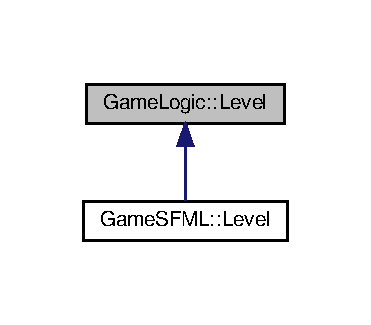
\includegraphics[width=178pt]{classGameLogic_1_1Level__inherit__graph}
\end{center}
\end{figure}


Collaboration diagram for Game\+Logic\+:\+:Level\+:
\nopagebreak
\begin{figure}[H]
\begin{center}
\leavevmode
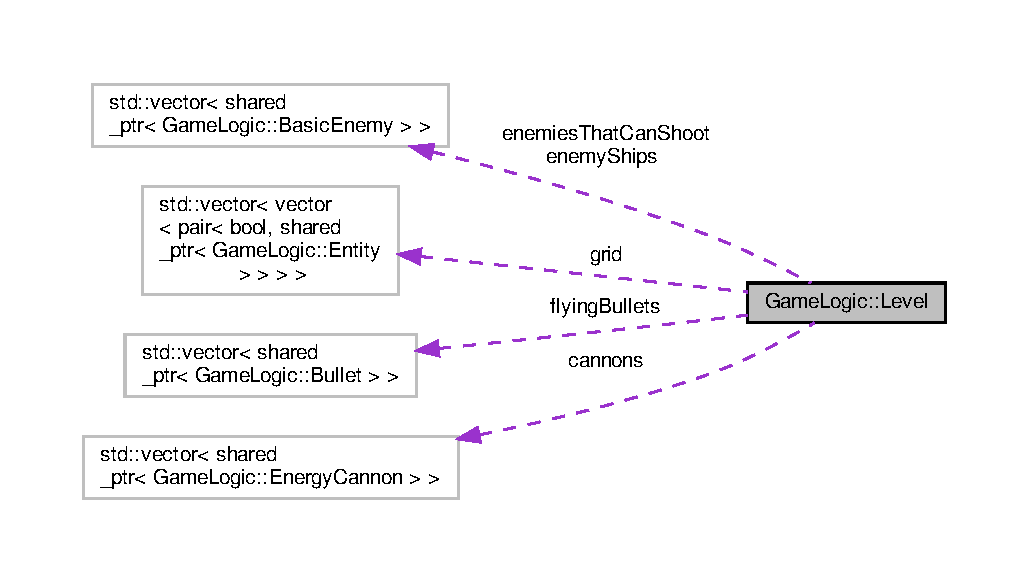
\includegraphics[width=350pt]{classGameLogic_1_1Level__coll__graph}
\end{center}
\end{figure}
\subsection*{Public Member Functions}
\begin{DoxyCompactItemize}
\item 
void \hyperlink{classGameLogic_1_1Level_a4d6e8cd499b0d78a36f7a2f89f221456}{add\+Enemy\+Ship} (shared\+\_\+ptr$<$ \hyperlink{classGameLogic_1_1BasicEnemy}{Basic\+Enemy} $>$ enemy)
\begin{DoxyCompactList}\small\item\em Adds a new enemy ship to the level. \end{DoxyCompactList}\item 
void \hyperlink{classGameLogic_1_1Level_a0d3d5db9311e281b7161c4daff692249}{update\+Grid} ()
\begin{DoxyCompactList}\small\item\em Updates the grid to accurately represent the current state of the game. \end{DoxyCompactList}\item 
void \hyperlink{classGameLogic_1_1Level_a42e42fda28e7f43286d9beb166d1e3f9}{add\+Row} (vector$<$ pair$<$ bool, shared\+\_\+ptr$<$ \hyperlink{classGameLogic_1_1Entity}{Entity} $>$$>$$>$ row)
\begin{DoxyCompactList}\small\item\em Adds a new row to the grid. \end{DoxyCompactList}\item 
int \hyperlink{classGameLogic_1_1Level_a3c233a241cf2ea7a231186acf2301ec3}{get\+Grid\+\_\+x} () const
\begin{DoxyCompactList}\small\item\em Getter for the max x value of the grid set by the grid\+\_\+x value of the class. \end{DoxyCompactList}\item 
void \hyperlink{classGameLogic_1_1Level_ac5f2066f82041e2222b79c427055f424}{set\+Grid\+\_\+x} (int grid\+\_\+x)
\begin{DoxyCompactList}\small\item\em Setter for the max x value of the grid set by the grid\+\_\+x value of the class. \end{DoxyCompactList}\item 
int \hyperlink{classGameLogic_1_1Level_a72e96cb117a1de175c2c91eb953f5b74}{get\+Grid\+\_\+y} () const
\begin{DoxyCompactList}\small\item\em Getter for the max y value of the grid set by the grid\+\_\+y value of the class. \end{DoxyCompactList}\item 
void \hyperlink{classGameLogic_1_1Level_a23edca6119a73f28b7823f1d6c1df2d6}{set\+Grid\+\_\+y} (int grid\+\_\+y)
\begin{DoxyCompactList}\small\item\em Setter for the max y value of the grid set by the grid\+\_\+y value of the class. \end{DoxyCompactList}\item 
void \hyperlink{classGameLogic_1_1Level_a9945b2baf78f44ff61f189846cc59c7a}{add\+Entity\+To\+Grid} (shared\+\_\+ptr$<$ \hyperlink{classGameLogic_1_1Entity}{Entity} $>$ entity)
\begin{DoxyCompactList}\small\item\em Adds a new entity to the grid. \end{DoxyCompactList}\item 
shared\+\_\+ptr$<$ \hyperlink{classGameLogic_1_1Player}{Player} $>$ \hyperlink{classGameLogic_1_1Level_a76420d9e37505a2e5cbbbe8c4f57adbe}{get\+Player} () const
\begin{DoxyCompactList}\small\item\em Function to get the shared pointer to the player. \end{DoxyCompactList}\item 
void \hyperlink{classGameLogic_1_1Level_a418ab1b60ad2d35ad5983a0ec596dce6}{set\+Player} (shared\+\_\+ptr$<$ \hyperlink{classGameLogic_1_1Player}{Player} $>$ player)
\begin{DoxyCompactList}\small\item\em Sets the player to the shared pointer of the player entity. \end{DoxyCompactList}\item 
virtual void \hyperlink{classGameLogic_1_1Level_a72f5b36a0254821aabaaafa48834998b}{update} ()
\begin{DoxyCompactList}\small\item\em Updates the level. \end{DoxyCompactList}\item 
bool \hyperlink{classGameLogic_1_1Level_ab4496926ad24689d101de4a2e3702149}{game\+Over} ()
\begin{DoxyCompactList}\small\item\em Checks whether one of the game over conditions is triggered. \end{DoxyCompactList}\item 
bool \hyperlink{classGameLogic_1_1Level_a045b9a34d69596868df7c66f47d6912e}{check\+If\+Lowest\+Enemy} (shared\+\_\+ptr$<$ \hyperlink{classGameLogic_1_1BasicEnemy}{Basic\+Enemy} $>$ checked\+Enemy)
\begin{DoxyCompactList}\small\item\em Checks if there are no enemies below the one checked. \end{DoxyCompactList}\item 
vector$<$ shared\+\_\+ptr$<$ \hyperlink{classGameLogic_1_1Entity}{Entity} $>$ $>$ \hyperlink{classGameLogic_1_1Level_aa6b01a37c08040974534c00031e8cbed}{get\+Removable\+Entities} ()
\begin{DoxyCompactList}\small\item\em Returns a vector of entities that should be deleted. \end{DoxyCompactList}\item 
void \hyperlink{classGameLogic_1_1Level_a6f581d8c053ae5a9d5b6a333b455038f}{remove\+Removable\+Entities} ()
\begin{DoxyCompactList}\small\item\em Deletes all entities that aren\textquotesingle{}t used anymore. \end{DoxyCompactList}\item 
bool \hyperlink{classGameLogic_1_1Level_aaf7dd085cfe83d8c59f224f8d0acc6ec}{check\+Collision} (shared\+\_\+ptr$<$ \hyperlink{classGameLogic_1_1Entity}{Entity} $>$ entity1, shared\+\_\+ptr$<$ \hyperlink{classGameLogic_1_1Entity}{Entity} $>$ entity2)
\begin{DoxyCompactList}\small\item\em Checks if 2 entities collide. \end{DoxyCompactList}\item 
pair$<$ double, double $>$ \hyperlink{classGameLogic_1_1Level_ae6edaa461fc6cd170387a3d7b3e16d1f}{get\+Upper\+Left\+Corner} (shared\+\_\+ptr$<$ \hyperlink{classGameLogic_1_1Entity}{Entity} $>$ entity)
\begin{DoxyCompactList}\small\item\em Returns the upperleft corner of the entity. \end{DoxyCompactList}\item 
pair$<$ double, double $>$ \hyperlink{classGameLogic_1_1Level_a0a4b3dacec30ac1de1a2170082a9d799}{get\+Lower\+Right\+Corner} (shared\+\_\+ptr$<$ \hyperlink{classGameLogic_1_1Entity}{Entity} $>$ entity)
\begin{DoxyCompactList}\small\item\em Returns the lowerright corner of the entity. \end{DoxyCompactList}\item 
void \hyperlink{classGameLogic_1_1Level_a9792c2e1bbb52931fe83355fcbb35b89}{check\+Collisions\+Of\+All} ()
\begin{DoxyCompactList}\small\item\em Check if any entities collide. \end{DoxyCompactList}\item 
void \hyperlink{classGameLogic_1_1Level_a728ab647770a64be071d4125d7bd5cd6}{add\+Cannon} (shared\+\_\+ptr$<$ \hyperlink{classGameLogic_1_1EnergyCannon}{Energy\+Cannon} $>$ new\+Cannon)
\begin{DoxyCompactList}\small\item\em Adds a new cannon to the level. \end{DoxyCompactList}\item 
shared\+\_\+ptr$<$ \hyperlink{classGameLogic_1_1Entity}{Entity} $>$ \hyperlink{classGameLogic_1_1Level_afbe96c6615ae2df79dd3ce90fcedf83a}{get\+Entity\+In\+Grid} (int gridY, int gridX)
\begin{DoxyCompactList}\small\item\em Returns the entity at the given position in the grid. \end{DoxyCompactList}\item 
int \hyperlink{classGameLogic_1_1Level_a393075a2f768bf13c35ca338d1785694}{get\+Basic\+Enemy\+Width} () const
\begin{DoxyCompactList}\small\item\em Getter for the width of the basic enemy. \end{DoxyCompactList}\item 
int \hyperlink{classGameLogic_1_1Level_a5ff5361f7a4f4ff3ac58c95dfdc2341a}{get\+Basic\+Enemy\+Height} () const
\begin{DoxyCompactList}\small\item\em Getter for the height of the basic enemy. \end{DoxyCompactList}\item 
int \hyperlink{classGameLogic_1_1Level_a3e891e1ebca3e64b0fcf85ec6b50ee44}{get\+Player\+Width} () const
\begin{DoxyCompactList}\small\item\em Getter for the width of the player. \end{DoxyCompactList}\item 
int \hyperlink{classGameLogic_1_1Level_a6fdeff89393edde1156f75ccab640c79}{get\+Player\+Height} () const
\begin{DoxyCompactList}\small\item\em Getter for the height of the player. \end{DoxyCompactList}\item 
int \hyperlink{classGameLogic_1_1Level_a3986fbece7460c76852b0455b433b06d}{get\+Basic\+Enemy\+Bullet\+Width} () const
\begin{DoxyCompactList}\small\item\em Getter for the width of the basic enemy bullet. \end{DoxyCompactList}\item 
int \hyperlink{classGameLogic_1_1Level_a5063897104bbf7ff1f2d173cc37a0f57}{get\+Basic\+Enemy\+Bullet\+Height} () const
\begin{DoxyCompactList}\small\item\em Getter for the height of the basic enemy bullet. \end{DoxyCompactList}\item 
int \hyperlink{classGameLogic_1_1Level_a20cbcb471e2060a0024c5f7a055a85ce}{get\+Double\+Shot\+Enemy\+Width} () const
\begin{DoxyCompactList}\small\item\em Getter for the width of the double shot enemy. \end{DoxyCompactList}\item 
int \hyperlink{classGameLogic_1_1Level_a3196aa721c3d7b09be321ef3bbf0c5e9}{get\+Double\+Shot\+Enemy\+Height} () const
\begin{DoxyCompactList}\small\item\em Getter for the height of the double shot enemy. \end{DoxyCompactList}\item 
int \hyperlink{classGameLogic_1_1Level_a423e12a9f87441175f1ae449096ee997}{get\+Cannon\+Width} () const
\begin{DoxyCompactList}\small\item\em Getter for the width of the cannon. \end{DoxyCompactList}\item 
int \hyperlink{classGameLogic_1_1Level_ae66002e5cfd3f4404d34e1221505aeef}{get\+Cannon\+Height} () const
\begin{DoxyCompactList}\small\item\em Getter for the height of the cannon. \end{DoxyCompactList}\item 
int \hyperlink{classGameLogic_1_1Level_aba38362ae3b9b72fdb883dcf42965f78}{get\+Energy\+Bullet\+Width} () const
\begin{DoxyCompactList}\small\item\em Getter for the width of the energy bullet. \end{DoxyCompactList}\item 
int \hyperlink{classGameLogic_1_1Level_aa0b405c02ad398d415b2f378825d2c5b}{get\+Energy\+Bullet\+Height} () const
\begin{DoxyCompactList}\small\item\em Getter for the height of the energy bullet. \end{DoxyCompactList}\item 
virtual void \hyperlink{classGameLogic_1_1Level_ad9ac3fbb69cbfe7552a5ce8737a4cfd5}{create\+Player\+Bullet} (double y, double x)
\begin{DoxyCompactList}\small\item\em Creates a new \hyperlink{classGameLogic_1_1EnergyBullet}{Energy\+Bullet}. \end{DoxyCompactList}\item 
\mbox{\Hypertarget{classGameLogic_1_1Level_aab512e6cb8c1d3d4d703cc7e85d75391}\label{classGameLogic_1_1Level_aab512e6cb8c1d3d4d703cc7e85d75391}} 
bool {\bfseries won} ()
\end{DoxyCompactItemize}
\subsection*{Protected Attributes}
\begin{DoxyCompactItemize}
\item 
\mbox{\Hypertarget{classGameLogic_1_1Level_a14aad8e997f07e966fa9d51567c6b36e}\label{classGameLogic_1_1Level_a14aad8e997f07e966fa9d51567c6b36e}} 
vector$<$ shared\+\_\+ptr$<$ \hyperlink{classGameLogic_1_1BasicEnemy}{Basic\+Enemy} $>$ $>$ {\bfseries enemy\+Ships}
\item 
\mbox{\Hypertarget{classGameLogic_1_1Level_a4eef9e6b732bf31eabd60484f030ec5a}\label{classGameLogic_1_1Level_a4eef9e6b732bf31eabd60484f030ec5a}} 
vector$<$ vector$<$ pair$<$ bool, shared\+\_\+ptr$<$ \hyperlink{classGameLogic_1_1Entity}{Entity} $>$ $>$ $>$ $>$ {\bfseries grid}
\item 
\mbox{\Hypertarget{classGameLogic_1_1Level_af3af65172662d162fd1309f2c8286540}\label{classGameLogic_1_1Level_af3af65172662d162fd1309f2c8286540}} 
int {\bfseries grid\+\_\+x} = 9
\item 
\mbox{\Hypertarget{classGameLogic_1_1Level_aaef09f1a8d23bcea4d40716f43c85c8e}\label{classGameLogic_1_1Level_aaef09f1a8d23bcea4d40716f43c85c8e}} 
int {\bfseries grid\+\_\+y} = 7
\item 
\mbox{\Hypertarget{classGameLogic_1_1Level_a63e81c693d418fcc56cf38cb210ec812}\label{classGameLogic_1_1Level_a63e81c693d418fcc56cf38cb210ec812}} 
shared\+\_\+ptr$<$ \hyperlink{classGameLogic_1_1Player}{Player} $>$ {\bfseries player}
\item 
\mbox{\Hypertarget{classGameLogic_1_1Level_a1b28ec0b0e9b7e0344dccf60e5c2668b}\label{classGameLogic_1_1Level_a1b28ec0b0e9b7e0344dccf60e5c2668b}} 
vector$<$ shared\+\_\+ptr$<$ \hyperlink{classGameLogic_1_1BasicEnemy}{Basic\+Enemy} $>$ $>$ {\bfseries enemies\+That\+Can\+Shoot}
\item 
\mbox{\Hypertarget{classGameLogic_1_1Level_a6c4303f858a3f1348cf20ae826449bd8}\label{classGameLogic_1_1Level_a6c4303f858a3f1348cf20ae826449bd8}} 
vector$<$ shared\+\_\+ptr$<$ \hyperlink{classGameLogic_1_1Bullet}{Bullet} $>$ $>$ {\bfseries flying\+Bullets}
\item 
\mbox{\Hypertarget{classGameLogic_1_1Level_ad5b6c9ea691cc3e5389fa02b027b6514}\label{classGameLogic_1_1Level_ad5b6c9ea691cc3e5389fa02b027b6514}} 
vector$<$ shared\+\_\+ptr$<$ \hyperlink{classGameLogic_1_1EnergyCannon}{Energy\+Cannon} $>$ $>$ {\bfseries cannons}
\item 
\mbox{\Hypertarget{classGameLogic_1_1Level_a6a13203c180d5e383bb95322492456ce}\label{classGameLogic_1_1Level_a6a13203c180d5e383bb95322492456ce}} 
bool {\bfseries all\+Enemies\+Defeated} = false
\item 
\mbox{\Hypertarget{classGameLogic_1_1Level_ab119c656e9bfb54e0092b07ae220b3b9}\label{classGameLogic_1_1Level_ab119c656e9bfb54e0092b07ae220b3b9}} 
int {\bfseries basic\+Enemy\+Width} = 48
\item 
\mbox{\Hypertarget{classGameLogic_1_1Level_ae895c537c4e22d207106d2d6c53ecd41}\label{classGameLogic_1_1Level_ae895c537c4e22d207106d2d6c53ecd41}} 
int {\bfseries basic\+Enemy\+Height} = 29
\item 
\mbox{\Hypertarget{classGameLogic_1_1Level_a19ba7f37bfef1174c1db7e68edd8b599}\label{classGameLogic_1_1Level_a19ba7f37bfef1174c1db7e68edd8b599}} 
int {\bfseries player\+Width} = 44
\item 
\mbox{\Hypertarget{classGameLogic_1_1Level_a5e7307f10ad9f1560a878c43d349e942}\label{classGameLogic_1_1Level_a5e7307f10ad9f1560a878c43d349e942}} 
int {\bfseries player\+Height} = 36
\item 
\mbox{\Hypertarget{classGameLogic_1_1Level_a4c7f0cdc94125dc1c0f3ee79bb049188}\label{classGameLogic_1_1Level_a4c7f0cdc94125dc1c0f3ee79bb049188}} 
int {\bfseries basic\+Enemy\+Bullet\+Width} = 14
\item 
\mbox{\Hypertarget{classGameLogic_1_1Level_a433aed3c648f8bc0ec023056d8ecd749}\label{classGameLogic_1_1Level_a433aed3c648f8bc0ec023056d8ecd749}} 
int {\bfseries basic\+Enemy\+Bullet\+Height} = 25
\item 
\mbox{\Hypertarget{classGameLogic_1_1Level_a31ac35d0b155297039d13015e94875a6}\label{classGameLogic_1_1Level_a31ac35d0b155297039d13015e94875a6}} 
int {\bfseries double\+Shot\+Enemy\+Width} = 48
\item 
\mbox{\Hypertarget{classGameLogic_1_1Level_a41c7adbbfc65a64ce9b1e1dc3e2e0b67}\label{classGameLogic_1_1Level_a41c7adbbfc65a64ce9b1e1dc3e2e0b67}} 
int {\bfseries double\+Shot\+Enemy\+Height} = 27
\item 
\mbox{\Hypertarget{classGameLogic_1_1Level_a72aaffe845338ab603728c32876472b4}\label{classGameLogic_1_1Level_a72aaffe845338ab603728c32876472b4}} 
int {\bfseries cannon\+Width} = 36
\item 
\mbox{\Hypertarget{classGameLogic_1_1Level_a438cb19565dfc82ba9241d3417bcd07d}\label{classGameLogic_1_1Level_a438cb19565dfc82ba9241d3417bcd07d}} 
int {\bfseries cannon\+Height} = 34
\item 
\mbox{\Hypertarget{classGameLogic_1_1Level_ade726aed7ecf9c403b2f3a6dd2ba381e}\label{classGameLogic_1_1Level_ade726aed7ecf9c403b2f3a6dd2ba381e}} 
int {\bfseries energy\+Bullet\+Width} = 6
\item 
\mbox{\Hypertarget{classGameLogic_1_1Level_ac94d008bc4dec74b60b590ad22f95a75}\label{classGameLogic_1_1Level_ac94d008bc4dec74b60b590ad22f95a75}} 
int {\bfseries energy\+Bullet\+Height} = 18
\end{DoxyCompactItemize}


\subsection{Member Function Documentation}
\mbox{\Hypertarget{classGameLogic_1_1Level_a728ab647770a64be071d4125d7bd5cd6}\label{classGameLogic_1_1Level_a728ab647770a64be071d4125d7bd5cd6}} 
\index{Game\+Logic\+::\+Level@{Game\+Logic\+::\+Level}!add\+Cannon@{add\+Cannon}}
\index{add\+Cannon@{add\+Cannon}!Game\+Logic\+::\+Level@{Game\+Logic\+::\+Level}}
\subsubsection{\texorpdfstring{add\+Cannon()}{addCannon()}}
{\footnotesize\ttfamily void Game\+Logic\+::\+Level\+::add\+Cannon (\begin{DoxyParamCaption}\item[{shared\+\_\+ptr$<$ \hyperlink{classGameLogic_1_1EnergyCannon}{Energy\+Cannon} $>$}]{new\+Cannon }\end{DoxyParamCaption})}

Adds a new cannon to the level. 
\begin{DoxyParams}{Parameters}
{\em new\+Cannon} & The cannon to add. \\
\hline
\end{DoxyParams}
\mbox{\Hypertarget{classGameLogic_1_1Level_a4d6e8cd499b0d78a36f7a2f89f221456}\label{classGameLogic_1_1Level_a4d6e8cd499b0d78a36f7a2f89f221456}} 
\index{Game\+Logic\+::\+Level@{Game\+Logic\+::\+Level}!add\+Enemy\+Ship@{add\+Enemy\+Ship}}
\index{add\+Enemy\+Ship@{add\+Enemy\+Ship}!Game\+Logic\+::\+Level@{Game\+Logic\+::\+Level}}
\subsubsection{\texorpdfstring{add\+Enemy\+Ship()}{addEnemyShip()}}
{\footnotesize\ttfamily void Game\+Logic\+::\+Level\+::add\+Enemy\+Ship (\begin{DoxyParamCaption}\item[{shared\+\_\+ptr$<$ \hyperlink{classGameLogic_1_1BasicEnemy}{Basic\+Enemy} $>$}]{enemy }\end{DoxyParamCaption})}

Function to add a new \hyperlink{classGameLogic_1_1Ship}{Ship} entity to the vector of enemy ships 
\begin{DoxyParams}{Parameters}
{\em ship} & shared pointer to the new enemy ship to add \\
\hline
\end{DoxyParams}
\mbox{\Hypertarget{classGameLogic_1_1Level_a9945b2baf78f44ff61f189846cc59c7a}\label{classGameLogic_1_1Level_a9945b2baf78f44ff61f189846cc59c7a}} 
\index{Game\+Logic\+::\+Level@{Game\+Logic\+::\+Level}!add\+Entity\+To\+Grid@{add\+Entity\+To\+Grid}}
\index{add\+Entity\+To\+Grid@{add\+Entity\+To\+Grid}!Game\+Logic\+::\+Level@{Game\+Logic\+::\+Level}}
\subsubsection{\texorpdfstring{add\+Entity\+To\+Grid()}{addEntityToGrid()}}
{\footnotesize\ttfamily void Game\+Logic\+::\+Level\+::add\+Entity\+To\+Grid (\begin{DoxyParamCaption}\item[{shared\+\_\+ptr$<$ \hyperlink{classGameLogic_1_1Entity}{Entity} $>$}]{entity }\end{DoxyParamCaption})}

Adds a new entity to the grid. Position in the grid is determined by the position value of the entity 
\begin{DoxyParams}{Parameters}
{\em entity} & Shared pointer to the entity that needs to be added \\
\hline
\end{DoxyParams}
\mbox{\Hypertarget{classGameLogic_1_1Level_a42e42fda28e7f43286d9beb166d1e3f9}\label{classGameLogic_1_1Level_a42e42fda28e7f43286d9beb166d1e3f9}} 
\index{Game\+Logic\+::\+Level@{Game\+Logic\+::\+Level}!add\+Row@{add\+Row}}
\index{add\+Row@{add\+Row}!Game\+Logic\+::\+Level@{Game\+Logic\+::\+Level}}
\subsubsection{\texorpdfstring{add\+Row()}{addRow()}}
{\footnotesize\ttfamily void Game\+Logic\+::\+Level\+::add\+Row (\begin{DoxyParamCaption}\item[{vector$<$ pair$<$ bool, shared\+\_\+ptr$<$ \hyperlink{classGameLogic_1_1Entity}{Entity} $>$$>$$>$}]{row }\end{DoxyParamCaption})}

Function adds a new row to the grid, mostly used to add a empty row when setting up the grid 
\begin{DoxyParams}{Parameters}
{\em row} & Vector that represents the row that gets added to the grid \\
\hline
\end{DoxyParams}
\mbox{\Hypertarget{classGameLogic_1_1Level_aaf7dd085cfe83d8c59f224f8d0acc6ec}\label{classGameLogic_1_1Level_aaf7dd085cfe83d8c59f224f8d0acc6ec}} 
\index{Game\+Logic\+::\+Level@{Game\+Logic\+::\+Level}!check\+Collision@{check\+Collision}}
\index{check\+Collision@{check\+Collision}!Game\+Logic\+::\+Level@{Game\+Logic\+::\+Level}}
\subsubsection{\texorpdfstring{check\+Collision()}{checkCollision()}}
{\footnotesize\ttfamily bool Game\+Logic\+::\+Level\+::check\+Collision (\begin{DoxyParamCaption}\item[{shared\+\_\+ptr$<$ \hyperlink{classGameLogic_1_1Entity}{Entity} $>$}]{entity1,  }\item[{shared\+\_\+ptr$<$ \hyperlink{classGameLogic_1_1Entity}{Entity} $>$}]{entity2 }\end{DoxyParamCaption})}

Returns a boolean that represents is 2 entities collide or not. 
\begin{DoxyParams}{Parameters}
{\em entity1} & First entity to check. \\
\hline
{\em entity2} & Second entity to check. \\
\hline
\end{DoxyParams}
\begin{DoxyReturn}{Returns}
Returns true if the entities collide. 
\end{DoxyReturn}
\mbox{\Hypertarget{classGameLogic_1_1Level_a9792c2e1bbb52931fe83355fcbb35b89}\label{classGameLogic_1_1Level_a9792c2e1bbb52931fe83355fcbb35b89}} 
\index{Game\+Logic\+::\+Level@{Game\+Logic\+::\+Level}!check\+Collisions\+Of\+All@{check\+Collisions\+Of\+All}}
\index{check\+Collisions\+Of\+All@{check\+Collisions\+Of\+All}!Game\+Logic\+::\+Level@{Game\+Logic\+::\+Level}}
\subsubsection{\texorpdfstring{check\+Collisions\+Of\+All()}{checkCollisionsOfAll()}}
{\footnotesize\ttfamily void Game\+Logic\+::\+Level\+::check\+Collisions\+Of\+All (\begin{DoxyParamCaption}{ }\end{DoxyParamCaption})}

Check if any entities collide. \mbox{\Hypertarget{classGameLogic_1_1Level_a045b9a34d69596868df7c66f47d6912e}\label{classGameLogic_1_1Level_a045b9a34d69596868df7c66f47d6912e}} 
\index{Game\+Logic\+::\+Level@{Game\+Logic\+::\+Level}!check\+If\+Lowest\+Enemy@{check\+If\+Lowest\+Enemy}}
\index{check\+If\+Lowest\+Enemy@{check\+If\+Lowest\+Enemy}!Game\+Logic\+::\+Level@{Game\+Logic\+::\+Level}}
\subsubsection{\texorpdfstring{check\+If\+Lowest\+Enemy()}{checkIfLowestEnemy()}}
{\footnotesize\ttfamily bool Game\+Logic\+::\+Level\+::check\+If\+Lowest\+Enemy (\begin{DoxyParamCaption}\item[{shared\+\_\+ptr$<$ \hyperlink{classGameLogic_1_1BasicEnemy}{Basic\+Enemy} $>$}]{checked\+Enemy }\end{DoxyParamCaption})}

Checks if there are no enemies below the one checked. 
\begin{DoxyParams}{Parameters}
{\em checked\+Enemy} & the enemy we want to check \\
\hline
\end{DoxyParams}
\begin{DoxyReturn}{Returns}
true if there are no enemies below it. 
\end{DoxyReturn}
\mbox{\Hypertarget{classGameLogic_1_1Level_ad9ac3fbb69cbfe7552a5ce8737a4cfd5}\label{classGameLogic_1_1Level_ad9ac3fbb69cbfe7552a5ce8737a4cfd5}} 
\index{Game\+Logic\+::\+Level@{Game\+Logic\+::\+Level}!create\+Player\+Bullet@{create\+Player\+Bullet}}
\index{create\+Player\+Bullet@{create\+Player\+Bullet}!Game\+Logic\+::\+Level@{Game\+Logic\+::\+Level}}
\subsubsection{\texorpdfstring{create\+Player\+Bullet()}{createPlayerBullet()}}
{\footnotesize\ttfamily void Game\+Logic\+::\+Level\+::create\+Player\+Bullet (\begin{DoxyParamCaption}\item[{double}]{y,  }\item[{double}]{x }\end{DoxyParamCaption})\hspace{0.3cm}{\ttfamily [virtual]}}

Creates a new \hyperlink{classGameLogic_1_1EnergyBullet}{Energy\+Bullet}. 
\begin{DoxyParams}{Parameters}
{\em y} & The Y coordinate of the cannon that fires the bullet. \\
\hline
{\em x} & The X coordinate of the cannon that fires the bullet. \\
\hline
\end{DoxyParams}


Reimplemented in \hyperlink{classGameSFML_1_1Level_adafff50ab250a1d85f1b1d48c085bac1}{Game\+S\+F\+M\+L\+::\+Level}.

\mbox{\Hypertarget{classGameLogic_1_1Level_ab4496926ad24689d101de4a2e3702149}\label{classGameLogic_1_1Level_ab4496926ad24689d101de4a2e3702149}} 
\index{Game\+Logic\+::\+Level@{Game\+Logic\+::\+Level}!game\+Over@{game\+Over}}
\index{game\+Over@{game\+Over}!Game\+Logic\+::\+Level@{Game\+Logic\+::\+Level}}
\subsubsection{\texorpdfstring{game\+Over()}{gameOver()}}
{\footnotesize\ttfamily bool Game\+Logic\+::\+Level\+::game\+Over (\begin{DoxyParamCaption}{ }\end{DoxyParamCaption})}

Function checks whether one of the game over/level over conditions is triggered (need to separate those) \begin{DoxyReturn}{Returns}
Boolean that equals true if one of the conditions is triggered 
\end{DoxyReturn}
\mbox{\Hypertarget{classGameLogic_1_1Level_a5063897104bbf7ff1f2d173cc37a0f57}\label{classGameLogic_1_1Level_a5063897104bbf7ff1f2d173cc37a0f57}} 
\index{Game\+Logic\+::\+Level@{Game\+Logic\+::\+Level}!get\+Basic\+Enemy\+Bullet\+Height@{get\+Basic\+Enemy\+Bullet\+Height}}
\index{get\+Basic\+Enemy\+Bullet\+Height@{get\+Basic\+Enemy\+Bullet\+Height}!Game\+Logic\+::\+Level@{Game\+Logic\+::\+Level}}
\subsubsection{\texorpdfstring{get\+Basic\+Enemy\+Bullet\+Height()}{getBasicEnemyBulletHeight()}}
{\footnotesize\ttfamily int Game\+Logic\+::\+Level\+::get\+Basic\+Enemy\+Bullet\+Height (\begin{DoxyParamCaption}{ }\end{DoxyParamCaption}) const}

Getter for the height of the basic enemy bullet. \begin{DoxyReturn}{Returns}
the height of the basic enemy bullet. 
\end{DoxyReturn}
\mbox{\Hypertarget{classGameLogic_1_1Level_a3986fbece7460c76852b0455b433b06d}\label{classGameLogic_1_1Level_a3986fbece7460c76852b0455b433b06d}} 
\index{Game\+Logic\+::\+Level@{Game\+Logic\+::\+Level}!get\+Basic\+Enemy\+Bullet\+Width@{get\+Basic\+Enemy\+Bullet\+Width}}
\index{get\+Basic\+Enemy\+Bullet\+Width@{get\+Basic\+Enemy\+Bullet\+Width}!Game\+Logic\+::\+Level@{Game\+Logic\+::\+Level}}
\subsubsection{\texorpdfstring{get\+Basic\+Enemy\+Bullet\+Width()}{getBasicEnemyBulletWidth()}}
{\footnotesize\ttfamily int Game\+Logic\+::\+Level\+::get\+Basic\+Enemy\+Bullet\+Width (\begin{DoxyParamCaption}{ }\end{DoxyParamCaption}) const}

Getter for the width of the basic enemy bullet. \begin{DoxyReturn}{Returns}
the width of the basic enemy bullet. 
\end{DoxyReturn}
\mbox{\Hypertarget{classGameLogic_1_1Level_a5ff5361f7a4f4ff3ac58c95dfdc2341a}\label{classGameLogic_1_1Level_a5ff5361f7a4f4ff3ac58c95dfdc2341a}} 
\index{Game\+Logic\+::\+Level@{Game\+Logic\+::\+Level}!get\+Basic\+Enemy\+Height@{get\+Basic\+Enemy\+Height}}
\index{get\+Basic\+Enemy\+Height@{get\+Basic\+Enemy\+Height}!Game\+Logic\+::\+Level@{Game\+Logic\+::\+Level}}
\subsubsection{\texorpdfstring{get\+Basic\+Enemy\+Height()}{getBasicEnemyHeight()}}
{\footnotesize\ttfamily int Game\+Logic\+::\+Level\+::get\+Basic\+Enemy\+Height (\begin{DoxyParamCaption}{ }\end{DoxyParamCaption}) const}

Getter for the height of the basic enemy. \begin{DoxyReturn}{Returns}
the height of the basic enemy. 
\end{DoxyReturn}
\mbox{\Hypertarget{classGameLogic_1_1Level_a393075a2f768bf13c35ca338d1785694}\label{classGameLogic_1_1Level_a393075a2f768bf13c35ca338d1785694}} 
\index{Game\+Logic\+::\+Level@{Game\+Logic\+::\+Level}!get\+Basic\+Enemy\+Width@{get\+Basic\+Enemy\+Width}}
\index{get\+Basic\+Enemy\+Width@{get\+Basic\+Enemy\+Width}!Game\+Logic\+::\+Level@{Game\+Logic\+::\+Level}}
\subsubsection{\texorpdfstring{get\+Basic\+Enemy\+Width()}{getBasicEnemyWidth()}}
{\footnotesize\ttfamily int Game\+Logic\+::\+Level\+::get\+Basic\+Enemy\+Width (\begin{DoxyParamCaption}{ }\end{DoxyParamCaption}) const}

Getter for the width of the basic enemy. \begin{DoxyReturn}{Returns}
the width of the basic enemy. 
\end{DoxyReturn}
\mbox{\Hypertarget{classGameLogic_1_1Level_ae66002e5cfd3f4404d34e1221505aeef}\label{classGameLogic_1_1Level_ae66002e5cfd3f4404d34e1221505aeef}} 
\index{Game\+Logic\+::\+Level@{Game\+Logic\+::\+Level}!get\+Cannon\+Height@{get\+Cannon\+Height}}
\index{get\+Cannon\+Height@{get\+Cannon\+Height}!Game\+Logic\+::\+Level@{Game\+Logic\+::\+Level}}
\subsubsection{\texorpdfstring{get\+Cannon\+Height()}{getCannonHeight()}}
{\footnotesize\ttfamily int Game\+Logic\+::\+Level\+::get\+Cannon\+Height (\begin{DoxyParamCaption}{ }\end{DoxyParamCaption}) const}

Getter for the height of the cannon. \begin{DoxyReturn}{Returns}
the height of the cannon. 
\end{DoxyReturn}
\mbox{\Hypertarget{classGameLogic_1_1Level_a423e12a9f87441175f1ae449096ee997}\label{classGameLogic_1_1Level_a423e12a9f87441175f1ae449096ee997}} 
\index{Game\+Logic\+::\+Level@{Game\+Logic\+::\+Level}!get\+Cannon\+Width@{get\+Cannon\+Width}}
\index{get\+Cannon\+Width@{get\+Cannon\+Width}!Game\+Logic\+::\+Level@{Game\+Logic\+::\+Level}}
\subsubsection{\texorpdfstring{get\+Cannon\+Width()}{getCannonWidth()}}
{\footnotesize\ttfamily int Game\+Logic\+::\+Level\+::get\+Cannon\+Width (\begin{DoxyParamCaption}{ }\end{DoxyParamCaption}) const}

Getter for the width of the cannon. \begin{DoxyReturn}{Returns}
the width of the cannon. 
\end{DoxyReturn}
\mbox{\Hypertarget{classGameLogic_1_1Level_a3196aa721c3d7b09be321ef3bbf0c5e9}\label{classGameLogic_1_1Level_a3196aa721c3d7b09be321ef3bbf0c5e9}} 
\index{Game\+Logic\+::\+Level@{Game\+Logic\+::\+Level}!get\+Double\+Shot\+Enemy\+Height@{get\+Double\+Shot\+Enemy\+Height}}
\index{get\+Double\+Shot\+Enemy\+Height@{get\+Double\+Shot\+Enemy\+Height}!Game\+Logic\+::\+Level@{Game\+Logic\+::\+Level}}
\subsubsection{\texorpdfstring{get\+Double\+Shot\+Enemy\+Height()}{getDoubleShotEnemyHeight()}}
{\footnotesize\ttfamily int Game\+Logic\+::\+Level\+::get\+Double\+Shot\+Enemy\+Height (\begin{DoxyParamCaption}{ }\end{DoxyParamCaption}) const}

Getter for the height of the double shot enemy. \begin{DoxyReturn}{Returns}
the height of the double shot enemy. 
\end{DoxyReturn}
\mbox{\Hypertarget{classGameLogic_1_1Level_a20cbcb471e2060a0024c5f7a055a85ce}\label{classGameLogic_1_1Level_a20cbcb471e2060a0024c5f7a055a85ce}} 
\index{Game\+Logic\+::\+Level@{Game\+Logic\+::\+Level}!get\+Double\+Shot\+Enemy\+Width@{get\+Double\+Shot\+Enemy\+Width}}
\index{get\+Double\+Shot\+Enemy\+Width@{get\+Double\+Shot\+Enemy\+Width}!Game\+Logic\+::\+Level@{Game\+Logic\+::\+Level}}
\subsubsection{\texorpdfstring{get\+Double\+Shot\+Enemy\+Width()}{getDoubleShotEnemyWidth()}}
{\footnotesize\ttfamily int Game\+Logic\+::\+Level\+::get\+Double\+Shot\+Enemy\+Width (\begin{DoxyParamCaption}{ }\end{DoxyParamCaption}) const}

Getter for the width of the double shot enemy. \begin{DoxyReturn}{Returns}
the width of the double shot enemy. 
\end{DoxyReturn}
\mbox{\Hypertarget{classGameLogic_1_1Level_aa0b405c02ad398d415b2f378825d2c5b}\label{classGameLogic_1_1Level_aa0b405c02ad398d415b2f378825d2c5b}} 
\index{Game\+Logic\+::\+Level@{Game\+Logic\+::\+Level}!get\+Energy\+Bullet\+Height@{get\+Energy\+Bullet\+Height}}
\index{get\+Energy\+Bullet\+Height@{get\+Energy\+Bullet\+Height}!Game\+Logic\+::\+Level@{Game\+Logic\+::\+Level}}
\subsubsection{\texorpdfstring{get\+Energy\+Bullet\+Height()}{getEnergyBulletHeight()}}
{\footnotesize\ttfamily int Game\+Logic\+::\+Level\+::get\+Energy\+Bullet\+Height (\begin{DoxyParamCaption}{ }\end{DoxyParamCaption}) const}

Getter for the height of the energy bullet. \begin{DoxyReturn}{Returns}
the height of the energy bullet. 
\end{DoxyReturn}
\mbox{\Hypertarget{classGameLogic_1_1Level_aba38362ae3b9b72fdb883dcf42965f78}\label{classGameLogic_1_1Level_aba38362ae3b9b72fdb883dcf42965f78}} 
\index{Game\+Logic\+::\+Level@{Game\+Logic\+::\+Level}!get\+Energy\+Bullet\+Width@{get\+Energy\+Bullet\+Width}}
\index{get\+Energy\+Bullet\+Width@{get\+Energy\+Bullet\+Width}!Game\+Logic\+::\+Level@{Game\+Logic\+::\+Level}}
\subsubsection{\texorpdfstring{get\+Energy\+Bullet\+Width()}{getEnergyBulletWidth()}}
{\footnotesize\ttfamily int Game\+Logic\+::\+Level\+::get\+Energy\+Bullet\+Width (\begin{DoxyParamCaption}{ }\end{DoxyParamCaption}) const}

Getter for the width of the energy bullet. \begin{DoxyReturn}{Returns}
the width of the energy bullet. 
\end{DoxyReturn}
\mbox{\Hypertarget{classGameLogic_1_1Level_afbe96c6615ae2df79dd3ce90fcedf83a}\label{classGameLogic_1_1Level_afbe96c6615ae2df79dd3ce90fcedf83a}} 
\index{Game\+Logic\+::\+Level@{Game\+Logic\+::\+Level}!get\+Entity\+In\+Grid@{get\+Entity\+In\+Grid}}
\index{get\+Entity\+In\+Grid@{get\+Entity\+In\+Grid}!Game\+Logic\+::\+Level@{Game\+Logic\+::\+Level}}
\subsubsection{\texorpdfstring{get\+Entity\+In\+Grid()}{getEntityInGrid()}}
{\footnotesize\ttfamily shared\+\_\+ptr$<$ \hyperlink{classGameLogic_1_1Entity}{Entity} $>$ Game\+Logic\+::\+Level\+::get\+Entity\+In\+Grid (\begin{DoxyParamCaption}\item[{int}]{gridY,  }\item[{int}]{gridX }\end{DoxyParamCaption})}

Returns the entity at the given position in the grid. 
\begin{DoxyParams}{Parameters}
{\em gridY} & Y coordinate of the grid. \\
\hline
{\em gridX} & X coordinate of the grid. \\
\hline
\end{DoxyParams}
\begin{DoxyReturn}{Returns}
If entity found a pointer to it, otherwise a nullpointer. 
\end{DoxyReturn}
\mbox{\Hypertarget{classGameLogic_1_1Level_a3c233a241cf2ea7a231186acf2301ec3}\label{classGameLogic_1_1Level_a3c233a241cf2ea7a231186acf2301ec3}} 
\index{Game\+Logic\+::\+Level@{Game\+Logic\+::\+Level}!get\+Grid\+\_\+x@{get\+Grid\+\_\+x}}
\index{get\+Grid\+\_\+x@{get\+Grid\+\_\+x}!Game\+Logic\+::\+Level@{Game\+Logic\+::\+Level}}
\subsubsection{\texorpdfstring{get\+Grid\+\_\+x()}{getGrid\_x()}}
{\footnotesize\ttfamily int Game\+Logic\+::\+Level\+::get\+Grid\+\_\+x (\begin{DoxyParamCaption}{ }\end{DoxyParamCaption}) const}

\begin{DoxyReturn}{Returns}
Integer that is the max x value of the grid 
\end{DoxyReturn}
\mbox{\Hypertarget{classGameLogic_1_1Level_a72e96cb117a1de175c2c91eb953f5b74}\label{classGameLogic_1_1Level_a72e96cb117a1de175c2c91eb953f5b74}} 
\index{Game\+Logic\+::\+Level@{Game\+Logic\+::\+Level}!get\+Grid\+\_\+y@{get\+Grid\+\_\+y}}
\index{get\+Grid\+\_\+y@{get\+Grid\+\_\+y}!Game\+Logic\+::\+Level@{Game\+Logic\+::\+Level}}
\subsubsection{\texorpdfstring{get\+Grid\+\_\+y()}{getGrid\_y()}}
{\footnotesize\ttfamily int Game\+Logic\+::\+Level\+::get\+Grid\+\_\+y (\begin{DoxyParamCaption}{ }\end{DoxyParamCaption}) const}

\begin{DoxyReturn}{Returns}
Integer that is the max y value of the grid 
\end{DoxyReturn}
\mbox{\Hypertarget{classGameLogic_1_1Level_a0a4b3dacec30ac1de1a2170082a9d799}\label{classGameLogic_1_1Level_a0a4b3dacec30ac1de1a2170082a9d799}} 
\index{Game\+Logic\+::\+Level@{Game\+Logic\+::\+Level}!get\+Lower\+Right\+Corner@{get\+Lower\+Right\+Corner}}
\index{get\+Lower\+Right\+Corner@{get\+Lower\+Right\+Corner}!Game\+Logic\+::\+Level@{Game\+Logic\+::\+Level}}
\subsubsection{\texorpdfstring{get\+Lower\+Right\+Corner()}{getLowerRightCorner()}}
{\footnotesize\ttfamily pair$<$ double, double $>$ Game\+Logic\+::\+Level\+::get\+Lower\+Right\+Corner (\begin{DoxyParamCaption}\item[{shared\+\_\+ptr$<$ \hyperlink{classGameLogic_1_1Entity}{Entity} $>$}]{entity }\end{DoxyParamCaption})}

Returns the lowerright corner of the entity in the forms of a pair with the y coordinate first. 
\begin{DoxyParams}{Parameters}
{\em entity} & The entity we want the corner of. \\
\hline
\end{DoxyParams}
\begin{DoxyReturn}{Returns}
The corner in the form of a pair with the y coordinate first. 
\end{DoxyReturn}
\mbox{\Hypertarget{classGameLogic_1_1Level_a76420d9e37505a2e5cbbbe8c4f57adbe}\label{classGameLogic_1_1Level_a76420d9e37505a2e5cbbbe8c4f57adbe}} 
\index{Game\+Logic\+::\+Level@{Game\+Logic\+::\+Level}!get\+Player@{get\+Player}}
\index{get\+Player@{get\+Player}!Game\+Logic\+::\+Level@{Game\+Logic\+::\+Level}}
\subsubsection{\texorpdfstring{get\+Player()}{getPlayer()}}
{\footnotesize\ttfamily shared\+\_\+ptr$<$ \hyperlink{classGameLogic_1_1Player}{Player} $>$ Game\+Logic\+::\+Level\+::get\+Player (\begin{DoxyParamCaption}{ }\end{DoxyParamCaption}) const}

Returns the shared pointer to the player entity \begin{DoxyReturn}{Returns}
The shared pointer to the player entity 
\end{DoxyReturn}
\mbox{\Hypertarget{classGameLogic_1_1Level_a6fdeff89393edde1156f75ccab640c79}\label{classGameLogic_1_1Level_a6fdeff89393edde1156f75ccab640c79}} 
\index{Game\+Logic\+::\+Level@{Game\+Logic\+::\+Level}!get\+Player\+Height@{get\+Player\+Height}}
\index{get\+Player\+Height@{get\+Player\+Height}!Game\+Logic\+::\+Level@{Game\+Logic\+::\+Level}}
\subsubsection{\texorpdfstring{get\+Player\+Height()}{getPlayerHeight()}}
{\footnotesize\ttfamily int Game\+Logic\+::\+Level\+::get\+Player\+Height (\begin{DoxyParamCaption}{ }\end{DoxyParamCaption}) const}

Getter for the height of the player. \begin{DoxyReturn}{Returns}
the height of the player. 
\end{DoxyReturn}
\mbox{\Hypertarget{classGameLogic_1_1Level_a3e891e1ebca3e64b0fcf85ec6b50ee44}\label{classGameLogic_1_1Level_a3e891e1ebca3e64b0fcf85ec6b50ee44}} 
\index{Game\+Logic\+::\+Level@{Game\+Logic\+::\+Level}!get\+Player\+Width@{get\+Player\+Width}}
\index{get\+Player\+Width@{get\+Player\+Width}!Game\+Logic\+::\+Level@{Game\+Logic\+::\+Level}}
\subsubsection{\texorpdfstring{get\+Player\+Width()}{getPlayerWidth()}}
{\footnotesize\ttfamily int Game\+Logic\+::\+Level\+::get\+Player\+Width (\begin{DoxyParamCaption}{ }\end{DoxyParamCaption}) const}

Getter for the width of the player. \begin{DoxyReturn}{Returns}
the width of the player. 
\end{DoxyReturn}
\mbox{\Hypertarget{classGameLogic_1_1Level_aa6b01a37c08040974534c00031e8cbed}\label{classGameLogic_1_1Level_aa6b01a37c08040974534c00031e8cbed}} 
\index{Game\+Logic\+::\+Level@{Game\+Logic\+::\+Level}!get\+Removable\+Entities@{get\+Removable\+Entities}}
\index{get\+Removable\+Entities@{get\+Removable\+Entities}!Game\+Logic\+::\+Level@{Game\+Logic\+::\+Level}}
\subsubsection{\texorpdfstring{get\+Removable\+Entities()}{getRemovableEntities()}}
{\footnotesize\ttfamily vector$<$ shared\+\_\+ptr$<$ \hyperlink{classGameLogic_1_1Entity}{Entity} $>$ $>$ Game\+Logic\+::\+Level\+::get\+Removable\+Entities (\begin{DoxyParamCaption}{ }\end{DoxyParamCaption})}

Returns a vector of entities that should be deleted. \begin{DoxyReturn}{Returns}
A vector of entities that should be deleted. 
\end{DoxyReturn}
\mbox{\Hypertarget{classGameLogic_1_1Level_ae6edaa461fc6cd170387a3d7b3e16d1f}\label{classGameLogic_1_1Level_ae6edaa461fc6cd170387a3d7b3e16d1f}} 
\index{Game\+Logic\+::\+Level@{Game\+Logic\+::\+Level}!get\+Upper\+Left\+Corner@{get\+Upper\+Left\+Corner}}
\index{get\+Upper\+Left\+Corner@{get\+Upper\+Left\+Corner}!Game\+Logic\+::\+Level@{Game\+Logic\+::\+Level}}
\subsubsection{\texorpdfstring{get\+Upper\+Left\+Corner()}{getUpperLeftCorner()}}
{\footnotesize\ttfamily pair$<$ double, double $>$ Game\+Logic\+::\+Level\+::get\+Upper\+Left\+Corner (\begin{DoxyParamCaption}\item[{shared\+\_\+ptr$<$ \hyperlink{classGameLogic_1_1Entity}{Entity} $>$}]{entity }\end{DoxyParamCaption})}

Returns the upperleft corner of the entity in the forms of a pair with the y coordinate first. 
\begin{DoxyParams}{Parameters}
{\em entity} & The entity we want the corner of. \\
\hline
\end{DoxyParams}
\begin{DoxyReturn}{Returns}
The corner in the form of a pair with the y coordinate first. 
\end{DoxyReturn}
\mbox{\Hypertarget{classGameLogic_1_1Level_a6f581d8c053ae5a9d5b6a333b455038f}\label{classGameLogic_1_1Level_a6f581d8c053ae5a9d5b6a333b455038f}} 
\index{Game\+Logic\+::\+Level@{Game\+Logic\+::\+Level}!remove\+Removable\+Entities@{remove\+Removable\+Entities}}
\index{remove\+Removable\+Entities@{remove\+Removable\+Entities}!Game\+Logic\+::\+Level@{Game\+Logic\+::\+Level}}
\subsubsection{\texorpdfstring{remove\+Removable\+Entities()}{removeRemovableEntities()}}
{\footnotesize\ttfamily void Game\+Logic\+::\+Level\+::remove\+Removable\+Entities (\begin{DoxyParamCaption}{ }\end{DoxyParamCaption})}

Deletes all entities that aren\textquotesingle{}t used anymore. \mbox{\Hypertarget{classGameLogic_1_1Level_ac5f2066f82041e2222b79c427055f424}\label{classGameLogic_1_1Level_ac5f2066f82041e2222b79c427055f424}} 
\index{Game\+Logic\+::\+Level@{Game\+Logic\+::\+Level}!set\+Grid\+\_\+x@{set\+Grid\+\_\+x}}
\index{set\+Grid\+\_\+x@{set\+Grid\+\_\+x}!Game\+Logic\+::\+Level@{Game\+Logic\+::\+Level}}
\subsubsection{\texorpdfstring{set\+Grid\+\_\+x()}{setGrid\_x()}}
{\footnotesize\ttfamily void Game\+Logic\+::\+Level\+::set\+Grid\+\_\+x (\begin{DoxyParamCaption}\item[{int}]{grid\+\_\+x }\end{DoxyParamCaption})}


\begin{DoxyParams}{Parameters}
{\em grid\+\_\+x} & The integer value to set the max x value of the grid to. \\
\hline
\end{DoxyParams}
\mbox{\Hypertarget{classGameLogic_1_1Level_a23edca6119a73f28b7823f1d6c1df2d6}\label{classGameLogic_1_1Level_a23edca6119a73f28b7823f1d6c1df2d6}} 
\index{Game\+Logic\+::\+Level@{Game\+Logic\+::\+Level}!set\+Grid\+\_\+y@{set\+Grid\+\_\+y}}
\index{set\+Grid\+\_\+y@{set\+Grid\+\_\+y}!Game\+Logic\+::\+Level@{Game\+Logic\+::\+Level}}
\subsubsection{\texorpdfstring{set\+Grid\+\_\+y()}{setGrid\_y()}}
{\footnotesize\ttfamily void Game\+Logic\+::\+Level\+::set\+Grid\+\_\+y (\begin{DoxyParamCaption}\item[{int}]{grid\+\_\+y }\end{DoxyParamCaption})}


\begin{DoxyParams}{Parameters}
{\em grid\+\_\+y} & The integer value to set the max y value of the grid to. \\
\hline
\end{DoxyParams}
\mbox{\Hypertarget{classGameLogic_1_1Level_a418ab1b60ad2d35ad5983a0ec596dce6}\label{classGameLogic_1_1Level_a418ab1b60ad2d35ad5983a0ec596dce6}} 
\index{Game\+Logic\+::\+Level@{Game\+Logic\+::\+Level}!set\+Player@{set\+Player}}
\index{set\+Player@{set\+Player}!Game\+Logic\+::\+Level@{Game\+Logic\+::\+Level}}
\subsubsection{\texorpdfstring{set\+Player()}{setPlayer()}}
{\footnotesize\ttfamily void Game\+Logic\+::\+Level\+::set\+Player (\begin{DoxyParamCaption}\item[{shared\+\_\+ptr$<$ \hyperlink{classGameLogic_1_1Player}{Player} $>$}]{player }\end{DoxyParamCaption})}

Set the player, used only when parsing the level 
\begin{DoxyParams}{Parameters}
{\em player} & The shared pointer to the p\mbox{[}ayer \\
\hline
\end{DoxyParams}
\mbox{\Hypertarget{classGameLogic_1_1Level_a72f5b36a0254821aabaaafa48834998b}\label{classGameLogic_1_1Level_a72f5b36a0254821aabaaafa48834998b}} 
\index{Game\+Logic\+::\+Level@{Game\+Logic\+::\+Level}!update@{update}}
\index{update@{update}!Game\+Logic\+::\+Level@{Game\+Logic\+::\+Level}}
\subsubsection{\texorpdfstring{update()}{update()}}
{\footnotesize\ttfamily void Game\+Logic\+::\+Level\+::update (\begin{DoxyParamCaption}{ }\end{DoxyParamCaption})\hspace{0.3cm}{\ttfamily [virtual]}}

Function updates the level by moving all enemies to their next position by calling their move function, checking if enemies can fire and updating the grid. 

Reimplemented in \hyperlink{classGameSFML_1_1Level_ab98f7a9ceb040bef609c2c96990707ba}{Game\+S\+F\+M\+L\+::\+Level}.

\mbox{\Hypertarget{classGameLogic_1_1Level_a0d3d5db9311e281b7161c4daff692249}\label{classGameLogic_1_1Level_a0d3d5db9311e281b7161c4daff692249}} 
\index{Game\+Logic\+::\+Level@{Game\+Logic\+::\+Level}!update\+Grid@{update\+Grid}}
\index{update\+Grid@{update\+Grid}!Game\+Logic\+::\+Level@{Game\+Logic\+::\+Level}}
\subsubsection{\texorpdfstring{update\+Grid()}{updateGrid()}}
{\footnotesize\ttfamily void Game\+Logic\+::\+Level\+::update\+Grid (\begin{DoxyParamCaption}{ }\end{DoxyParamCaption})}

Function updates the state of the grid so all entity are in the correct position of the grid according to their position value 

The documentation for this class was generated from the following files\+:\begin{DoxyCompactItemize}
\item 
Game\+Logic/\+Include/\+Game\+Logic/Level.\+h\item 
Game\+Logic/src/Level.\+cpp\end{DoxyCompactItemize}

\hypertarget{classGameSFML_1_1Level}{}\section{Game\+S\+F\+ML\+:\+:Level Class Reference}
\label{classGameSFML_1_1Level}\index{Game\+S\+F\+M\+L\+::\+Level@{Game\+S\+F\+M\+L\+::\+Level}}


S\+F\+ML version of the \hyperlink{classGameSFML_1_1Level}{Level} class.  




{\ttfamily \#include $<$Level.\+h$>$}



Inheritance diagram for Game\+S\+F\+ML\+:\+:Level\+:\nopagebreak
\begin{figure}[H]
\begin{center}
\leavevmode
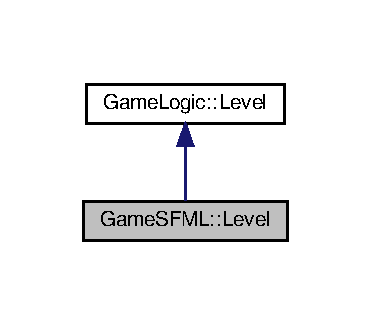
\includegraphics[width=178pt]{classGameSFML_1_1Level__inherit__graph}
\end{center}
\end{figure}


Collaboration diagram for Game\+S\+F\+ML\+:\+:Level\+:\nopagebreak
\begin{figure}[H]
\begin{center}
\leavevmode
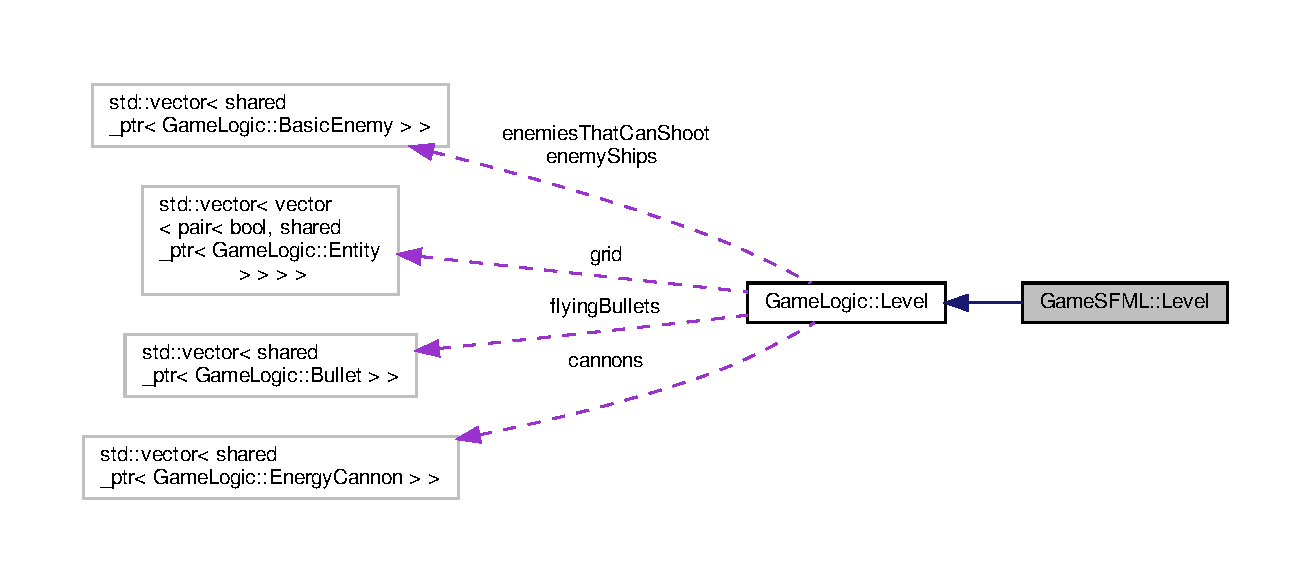
\includegraphics[width=350pt]{classGameSFML_1_1Level__coll__graph}
\end{center}
\end{figure}
\subsection*{Public Member Functions}
\begin{DoxyCompactItemize}
\item 
\hyperlink{classGameSFML_1_1Level_a68fb7b46bb5fde22cf16f6530d63efa7}{Level} (window\+\_\+ptr \&window)
\begin{DoxyCompactList}\small\item\em Constructor of the S\+F\+ML version of \hyperlink{classGameSFML_1_1Level}{Level}. \end{DoxyCompactList}\item 
void \hyperlink{classGameSFML_1_1Level_a102b4f351a97cde5a71a473b15126847}{draw} ()
\begin{DoxyCompactList}\small\item\em Calls the draw function of all entities. \end{DoxyCompactList}\item 
void \hyperlink{classGameSFML_1_1Level_ab98f7a9ceb040bef609c2c96990707ba}{update} () override
\begin{DoxyCompactList}\small\item\em Extends the \hyperlink{namespaceGameLogic}{Game\+Logic} version of the update function. \end{DoxyCompactList}\item 
void \hyperlink{classGameSFML_1_1Level_adafff50ab250a1d85f1b1d48c085bac1}{create\+Player\+Bullet} (double y, double x) override
\begin{DoxyCompactList}\small\item\em Creates a new \hyperlink{classGameSFML_1_1EnergyBullet}{Energy\+Bullet}. \end{DoxyCompactList}\end{DoxyCompactItemize}
\subsection*{Additional Inherited Members}


\subsection{Detailed Description}
S\+F\+ML version of the \hyperlink{classGameSFML_1_1Level}{Level} class. 

\subsection{Constructor \& Destructor Documentation}
\mbox{\Hypertarget{classGameSFML_1_1Level_a68fb7b46bb5fde22cf16f6530d63efa7}\label{classGameSFML_1_1Level_a68fb7b46bb5fde22cf16f6530d63efa7}} 
\index{Game\+S\+F\+M\+L\+::\+Level@{Game\+S\+F\+M\+L\+::\+Level}!Level@{Level}}
\index{Level@{Level}!Game\+S\+F\+M\+L\+::\+Level@{Game\+S\+F\+M\+L\+::\+Level}}
\subsubsection{\texorpdfstring{Level()}{Level()}}
{\footnotesize\ttfamily Game\+S\+F\+M\+L\+::\+Level\+::\+Level (\begin{DoxyParamCaption}\item[{window\+\_\+ptr \&}]{window }\end{DoxyParamCaption})\hspace{0.3cm}{\ttfamily [explicit]}}

Constructor of the S\+F\+ML version of \hyperlink{classGameSFML_1_1Level}{Level}. 
\begin{DoxyParams}{Parameters}
{\em window} & the current game window. \\
\hline
\end{DoxyParams}


\subsection{Member Function Documentation}
\mbox{\Hypertarget{classGameSFML_1_1Level_adafff50ab250a1d85f1b1d48c085bac1}\label{classGameSFML_1_1Level_adafff50ab250a1d85f1b1d48c085bac1}} 
\index{Game\+S\+F\+M\+L\+::\+Level@{Game\+S\+F\+M\+L\+::\+Level}!create\+Player\+Bullet@{create\+Player\+Bullet}}
\index{create\+Player\+Bullet@{create\+Player\+Bullet}!Game\+S\+F\+M\+L\+::\+Level@{Game\+S\+F\+M\+L\+::\+Level}}
\subsubsection{\texorpdfstring{create\+Player\+Bullet()}{createPlayerBullet()}}
{\footnotesize\ttfamily void Game\+S\+F\+M\+L\+::\+Level\+::create\+Player\+Bullet (\begin{DoxyParamCaption}\item[{double}]{y,  }\item[{double}]{x }\end{DoxyParamCaption})\hspace{0.3cm}{\ttfamily [override]}, {\ttfamily [virtual]}}

Creates a new \hyperlink{classGameSFML_1_1EnergyBullet}{Energy\+Bullet}. 
\begin{DoxyParams}{Parameters}
{\em y} & The Y coordinate of the cannon that fires the bullet. \\
\hline
{\em x} & The X coordinate of the cannon that fires the bullet. \\
\hline
\end{DoxyParams}


Reimplemented from \hyperlink{classGameLogic_1_1Level_ad9ac3fbb69cbfe7552a5ce8737a4cfd5}{Game\+Logic\+::\+Level}.

\mbox{\Hypertarget{classGameSFML_1_1Level_a102b4f351a97cde5a71a473b15126847}\label{classGameSFML_1_1Level_a102b4f351a97cde5a71a473b15126847}} 
\index{Game\+S\+F\+M\+L\+::\+Level@{Game\+S\+F\+M\+L\+::\+Level}!draw@{draw}}
\index{draw@{draw}!Game\+S\+F\+M\+L\+::\+Level@{Game\+S\+F\+M\+L\+::\+Level}}
\subsubsection{\texorpdfstring{draw()}{draw()}}
{\footnotesize\ttfamily void Game\+S\+F\+M\+L\+::\+Level\+::draw (\begin{DoxyParamCaption}{ }\end{DoxyParamCaption})}

Calls the draw function of all entities. \mbox{\Hypertarget{classGameSFML_1_1Level_ab98f7a9ceb040bef609c2c96990707ba}\label{classGameSFML_1_1Level_ab98f7a9ceb040bef609c2c96990707ba}} 
\index{Game\+S\+F\+M\+L\+::\+Level@{Game\+S\+F\+M\+L\+::\+Level}!update@{update}}
\index{update@{update}!Game\+S\+F\+M\+L\+::\+Level@{Game\+S\+F\+M\+L\+::\+Level}}
\subsubsection{\texorpdfstring{update()}{update()}}
{\footnotesize\ttfamily void Game\+S\+F\+M\+L\+::\+Level\+::update (\begin{DoxyParamCaption}{ }\end{DoxyParamCaption})\hspace{0.3cm}{\ttfamily [override]}, {\ttfamily [virtual]}}

Extends the \hyperlink{namespaceGameLogic}{Game\+Logic} version of the update function by creating new bullets if necessary, checking for collisions and removing removable entities. 

Reimplemented from \hyperlink{classGameLogic_1_1Level_a72f5b36a0254821aabaaafa48834998b}{Game\+Logic\+::\+Level}.



The documentation for this class was generated from the following files\+:\begin{DoxyCompactItemize}
\item 
S\+F\+M\+L/\+Include/Level.\+h\item 
S\+F\+M\+L/src/Level.\+cpp\end{DoxyCompactItemize}

\hypertarget{classGameSFML_1_1LevelParser}{}\section{Game\+S\+F\+ML\+:\+:Level\+Parser Class Reference}
\label{classGameSFML_1_1LevelParser}\index{Game\+S\+F\+M\+L\+::\+Level\+Parser@{Game\+S\+F\+M\+L\+::\+Level\+Parser}}


Class to help parse json files that represent the levels of the game.  




{\ttfamily \#include $<$Level\+Parser.\+h$>$}

\subsection*{Public Member Functions}
\begin{DoxyCompactItemize}
\item 
\hyperlink{classGameSFML_1_1LevelParser_a0c17b871d137992c985c8b52412af7d6}{Level\+Parser} (const string \&level\+File, Game\+S\+F\+M\+L\+::window\+\_\+ptr window)
\begin{DoxyCompactList}\small\item\em Constructor of the parser class. \end{DoxyCompactList}\item 
shared\+\_\+ptr$<$ \hyperlink{classGameSFML_1_1Level}{Game\+S\+F\+M\+L\+::\+Level} $>$ \hyperlink{classGameSFML_1_1LevelParser_a11eb8b7c40e1dad49b88de4d5c05bdbf}{parse\+Json} ()
\begin{DoxyCompactList}\small\item\em The actual parsing function. \end{DoxyCompactList}\end{DoxyCompactItemize}


\subsection{Constructor \& Destructor Documentation}
\mbox{\Hypertarget{classGameSFML_1_1LevelParser_a0c17b871d137992c985c8b52412af7d6}\label{classGameSFML_1_1LevelParser_a0c17b871d137992c985c8b52412af7d6}} 
\index{Game\+S\+F\+M\+L\+::\+Level\+Parser@{Game\+S\+F\+M\+L\+::\+Level\+Parser}!Level\+Parser@{Level\+Parser}}
\index{Level\+Parser@{Level\+Parser}!Game\+S\+F\+M\+L\+::\+Level\+Parser@{Game\+S\+F\+M\+L\+::\+Level\+Parser}}
\subsubsection{\texorpdfstring{Level\+Parser()}{LevelParser()}}
{\footnotesize\ttfamily Game\+S\+F\+M\+L\+::\+Level\+Parser\+::\+Level\+Parser (\begin{DoxyParamCaption}\item[{const string \&}]{level\+File,  }\item[{Game\+S\+F\+M\+L\+::window\+\_\+ptr}]{window }\end{DoxyParamCaption})}


\begin{DoxyParams}{Parameters}
{\em level\+File} & name of the json file that contains the level. \\
\hline
{\em window} & the current game window. \\
\hline
\end{DoxyParams}


\subsection{Member Function Documentation}
\mbox{\Hypertarget{classGameSFML_1_1LevelParser_a11eb8b7c40e1dad49b88de4d5c05bdbf}\label{classGameSFML_1_1LevelParser_a11eb8b7c40e1dad49b88de4d5c05bdbf}} 
\index{Game\+S\+F\+M\+L\+::\+Level\+Parser@{Game\+S\+F\+M\+L\+::\+Level\+Parser}!parse\+Json@{parse\+Json}}
\index{parse\+Json@{parse\+Json}!Game\+S\+F\+M\+L\+::\+Level\+Parser@{Game\+S\+F\+M\+L\+::\+Level\+Parser}}
\subsubsection{\texorpdfstring{parse\+Json()}{parseJson()}}
{\footnotesize\ttfamily shared\+\_\+ptr$<$ \hyperlink{classGameSFML_1_1Level}{Game\+S\+F\+M\+L\+::\+Level} $>$ Game\+S\+F\+M\+L\+::\+Level\+Parser\+::parse\+Json (\begin{DoxyParamCaption}{ }\end{DoxyParamCaption})}

Function parses the json file that was imported in the constructor \begin{DoxyReturn}{Returns}
Shared pointer to the created \hyperlink{classGameSFML_1_1Level}{Level} 
\end{DoxyReturn}


The documentation for this class was generated from the following files\+:\begin{DoxyCompactItemize}
\item 
S\+F\+M\+L/\+Include/Level\+Parser.\+h\item 
S\+F\+M\+L/src/Level\+Parser.\+cpp\end{DoxyCompactItemize}

\hypertarget{classGameSFML_1_1Player}{}\section{Game\+S\+F\+ML\+:\+:Player Class Reference}
\label{classGameSFML_1_1Player}\index{Game\+S\+F\+M\+L\+::\+Player@{Game\+S\+F\+M\+L\+::\+Player}}


S\+F\+ML version of the \hyperlink{classGameSFML_1_1Player}{Player} class.  




{\ttfamily \#include $<$Player.\+h$>$}



Inheritance diagram for Game\+S\+F\+ML\+:\+:Player\+:\nopagebreak
\begin{figure}[H]
\begin{center}
\leavevmode
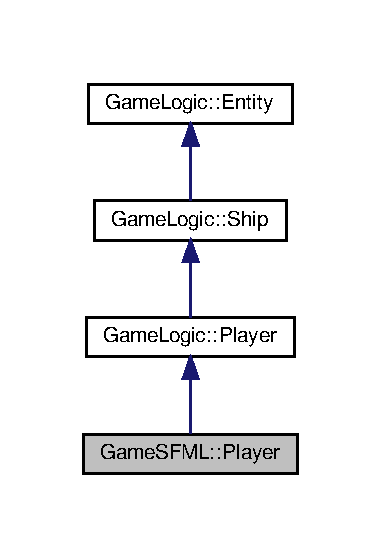
\includegraphics[width=183pt]{classGameSFML_1_1Player__inherit__graph}
\end{center}
\end{figure}


Collaboration diagram for Game\+S\+F\+ML\+:\+:Player\+:\nopagebreak
\begin{figure}[H]
\begin{center}
\leavevmode
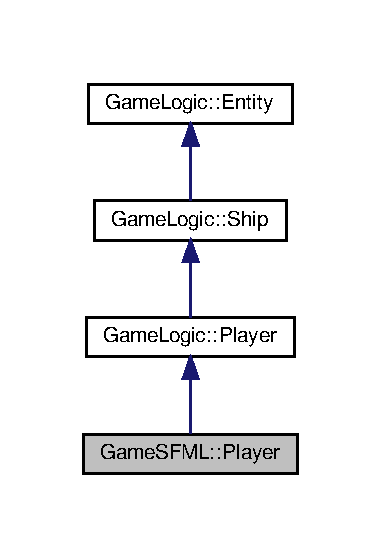
\includegraphics[width=183pt]{classGameSFML_1_1Player__coll__graph}
\end{center}
\end{figure}
\subsection*{Public Member Functions}
\begin{DoxyCompactItemize}
\item 
\hyperlink{classGameSFML_1_1Player_a3e69d607a6d700b103ed0454af91ad14}{Player} (const pair$<$ int, int $>$ \&position, double width, double height, const string \&file\+Name, Game\+S\+F\+M\+L\+::window\+\_\+ptr window)
\begin{DoxyCompactList}\small\item\em Constructor of the S\+F\+ML version of the player. \end{DoxyCompactList}\item 
void \hyperlink{classGameSFML_1_1Player_ac694755fafaffdf9432415452c7b9b5b}{draw} () override
\begin{DoxyCompactList}\small\item\em Updates the sprite and draws it to the window. \end{DoxyCompactList}\item 
void \hyperlink{classGameSFML_1_1Player_a8ef838c82c24aa99acd5dd1db17433c2}{update\+Sprite} ()
\begin{DoxyCompactList}\small\item\em Updates the sprite to the current position. \end{DoxyCompactList}\end{DoxyCompactItemize}
\subsection*{Additional Inherited Members}


\subsection{Detailed Description}
S\+F\+ML version of the \hyperlink{classGameSFML_1_1Player}{Player} class. 

\subsection{Constructor \& Destructor Documentation}
\mbox{\Hypertarget{classGameSFML_1_1Player_a3e69d607a6d700b103ed0454af91ad14}\label{classGameSFML_1_1Player_a3e69d607a6d700b103ed0454af91ad14}} 
\index{Game\+S\+F\+M\+L\+::\+Player@{Game\+S\+F\+M\+L\+::\+Player}!Player@{Player}}
\index{Player@{Player}!Game\+S\+F\+M\+L\+::\+Player@{Game\+S\+F\+M\+L\+::\+Player}}
\subsubsection{\texorpdfstring{Player()}{Player()}}
{\footnotesize\ttfamily Game\+S\+F\+M\+L\+::\+Player\+::\+Player (\begin{DoxyParamCaption}\item[{const pair$<$ int, int $>$ \&}]{position,  }\item[{double}]{width,  }\item[{double}]{height,  }\item[{const string \&}]{file\+Name,  }\item[{Game\+S\+F\+M\+L\+::window\+\_\+ptr}]{window }\end{DoxyParamCaption})}

Constructor of the S\+F\+ML version of the player. 
\begin{DoxyParams}{Parameters}
{\em position} & The position of the player in the grid \\
\hline
{\em width} & The width of the player \\
\hline
{\em height} & The height of the player \\
\hline
{\em file\+Name} & The name of the file that contains the player\textquotesingle{}s sprite. \\
\hline
{\em window} & The current game window. \\
\hline
\end{DoxyParams}


\subsection{Member Function Documentation}
\mbox{\Hypertarget{classGameSFML_1_1Player_ac694755fafaffdf9432415452c7b9b5b}\label{classGameSFML_1_1Player_ac694755fafaffdf9432415452c7b9b5b}} 
\index{Game\+S\+F\+M\+L\+::\+Player@{Game\+S\+F\+M\+L\+::\+Player}!draw@{draw}}
\index{draw@{draw}!Game\+S\+F\+M\+L\+::\+Player@{Game\+S\+F\+M\+L\+::\+Player}}
\subsubsection{\texorpdfstring{draw()}{draw()}}
{\footnotesize\ttfamily void Game\+S\+F\+M\+L\+::\+Player\+::draw (\begin{DoxyParamCaption}{ }\end{DoxyParamCaption})\hspace{0.3cm}{\ttfamily [override]}, {\ttfamily [virtual]}}

Updates the sprite and draws it to the window. 

Implements \hyperlink{classGameLogic_1_1Entity_adf23a7036cb99dfc6e33434018131da4}{Game\+Logic\+::\+Entity}.

\mbox{\Hypertarget{classGameSFML_1_1Player_a8ef838c82c24aa99acd5dd1db17433c2}\label{classGameSFML_1_1Player_a8ef838c82c24aa99acd5dd1db17433c2}} 
\index{Game\+S\+F\+M\+L\+::\+Player@{Game\+S\+F\+M\+L\+::\+Player}!update\+Sprite@{update\+Sprite}}
\index{update\+Sprite@{update\+Sprite}!Game\+S\+F\+M\+L\+::\+Player@{Game\+S\+F\+M\+L\+::\+Player}}
\subsubsection{\texorpdfstring{update\+Sprite()}{updateSprite()}}
{\footnotesize\ttfamily void Game\+S\+F\+M\+L\+::\+Player\+::update\+Sprite (\begin{DoxyParamCaption}{ }\end{DoxyParamCaption})}

Updates the sprite to the current position. 

The documentation for this class was generated from the following files\+:\begin{DoxyCompactItemize}
\item 
S\+F\+M\+L/\+Include/Player.\+h\item 
S\+F\+M\+L/src/Player.\+cpp\end{DoxyCompactItemize}

\hypertarget{classGameLogic_1_1Player}{}\section{Game\+Logic\+:\+:Player Class Reference}
\label{classGameLogic_1_1Player}\index{Game\+Logic\+::\+Player@{Game\+Logic\+::\+Player}}


Class to represent the player.  




{\ttfamily \#include $<$Player.\+h$>$}



Inheritance diagram for Game\+Logic\+:\+:Player\+:
\nopagebreak
\begin{figure}[H]
\begin{center}
\leavevmode
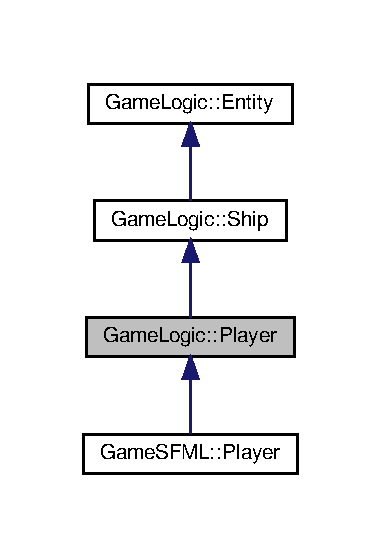
\includegraphics[width=183pt]{classGameLogic_1_1Player__inherit__graph}
\end{center}
\end{figure}


Collaboration diagram for Game\+Logic\+:\+:Player\+:
\nopagebreak
\begin{figure}[H]
\begin{center}
\leavevmode
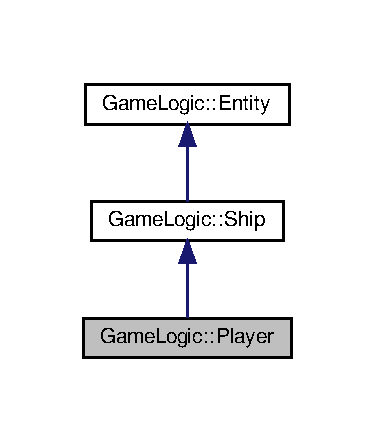
\includegraphics[width=180pt]{classGameLogic_1_1Player__coll__graph}
\end{center}
\end{figure}
\subsection*{Public Member Functions}
\begin{DoxyCompactItemize}
\item 
\hyperlink{classGameLogic_1_1Player_aeb3e4e8b10bf96de2543cafb683cf279}{Player} (const pair$<$ int, int $>$ \&position, double width, double height)
\begin{DoxyCompactList}\small\item\em Constructor for the \hyperlink{classGameLogic_1_1Player}{Player}. \end{DoxyCompactList}\item 
void \hyperlink{classGameLogic_1_1Player_a0595d93baa8c135aec8b9a6febc5d18c}{move\+Left} ()
\begin{DoxyCompactList}\small\item\em Moves the player left. \end{DoxyCompactList}\item 
void \hyperlink{classGameLogic_1_1Player_a42e5ab72dddca42e2ea2bbdeed63995e}{move\+Right} ()
\begin{DoxyCompactList}\small\item\em Moves the player right. \end{DoxyCompactList}\item 
bool \hyperlink{classGameLogic_1_1Player_a42d847fc003d1085a99aa0e72630aed2}{is\+Destroyed} () const
\begin{DoxyCompactList}\small\item\em Checks if player is destroyed. \end{DoxyCompactList}\item 
void \hyperlink{classGameLogic_1_1Player_a1f866a43d2db9e5f3dbeca80cbba28a7}{set\+Destroyed} (bool destroyed)
\begin{DoxyCompactList}\small\item\em Sets whether or not the player is destroyed. \end{DoxyCompactList}\end{DoxyCompactItemize}
\subsection*{Additional Inherited Members}


\subsection{Detailed Description}
Class represents the game logic version of the player 

\subsection{Constructor \& Destructor Documentation}
\mbox{\Hypertarget{classGameLogic_1_1Player_aeb3e4e8b10bf96de2543cafb683cf279}\label{classGameLogic_1_1Player_aeb3e4e8b10bf96de2543cafb683cf279}} 
\index{Game\+Logic\+::\+Player@{Game\+Logic\+::\+Player}!Player@{Player}}
\index{Player@{Player}!Game\+Logic\+::\+Player@{Game\+Logic\+::\+Player}}
\subsubsection{\texorpdfstring{Player()}{Player()}}
{\footnotesize\ttfamily Game\+Logic\+::\+Player\+::\+Player (\begin{DoxyParamCaption}\item[{const pair$<$ int, int $>$ \&}]{position,  }\item[{double}]{width,  }\item[{double}]{height }\end{DoxyParamCaption})\hspace{0.3cm}{\ttfamily [explicit]}}

The constructor for the \hyperlink{classGameLogic_1_1Player}{Player}. Sets the \hyperlink{classGameLogic_1_1Entity}{Entity} type to \hyperlink{classGameLogic_1_1Player}{Player} and sets the speed to 0.\+01 (speed might need balancing). 
\begin{DoxyParams}{Parameters}
{\em position} & The position of the player in the grid \\
\hline
{\em width} & The width of the player \\
\hline
{\em height} & The height of the player \\
\hline
\end{DoxyParams}


\subsection{Member Function Documentation}
\mbox{\Hypertarget{classGameLogic_1_1Player_a42d847fc003d1085a99aa0e72630aed2}\label{classGameLogic_1_1Player_a42d847fc003d1085a99aa0e72630aed2}} 
\index{Game\+Logic\+::\+Player@{Game\+Logic\+::\+Player}!is\+Destroyed@{is\+Destroyed}}
\index{is\+Destroyed@{is\+Destroyed}!Game\+Logic\+::\+Player@{Game\+Logic\+::\+Player}}
\subsubsection{\texorpdfstring{is\+Destroyed()}{isDestroyed()}}
{\footnotesize\ttfamily bool Game\+Logic\+::\+Player\+::is\+Destroyed (\begin{DoxyParamCaption}{ }\end{DoxyParamCaption}) const}

Checks if player is destroyed. Which usually ends in game over. \begin{DoxyReturn}{Returns}
Returns true if player is destroyed. 
\end{DoxyReturn}
\mbox{\Hypertarget{classGameLogic_1_1Player_a0595d93baa8c135aec8b9a6febc5d18c}\label{classGameLogic_1_1Player_a0595d93baa8c135aec8b9a6febc5d18c}} 
\index{Game\+Logic\+::\+Player@{Game\+Logic\+::\+Player}!move\+Left@{move\+Left}}
\index{move\+Left@{move\+Left}!Game\+Logic\+::\+Player@{Game\+Logic\+::\+Player}}
\subsubsection{\texorpdfstring{move\+Left()}{moveLeft()}}
{\footnotesize\ttfamily void Game\+Logic\+::\+Player\+::move\+Left (\begin{DoxyParamCaption}{ }\end{DoxyParamCaption})}

Function moves the player left by decreasing the x value in position and movingX. Checks if player not at the edge of the screen before moving. \mbox{\Hypertarget{classGameLogic_1_1Player_a42e5ab72dddca42e2ea2bbdeed63995e}\label{classGameLogic_1_1Player_a42e5ab72dddca42e2ea2bbdeed63995e}} 
\index{Game\+Logic\+::\+Player@{Game\+Logic\+::\+Player}!move\+Right@{move\+Right}}
\index{move\+Right@{move\+Right}!Game\+Logic\+::\+Player@{Game\+Logic\+::\+Player}}
\subsubsection{\texorpdfstring{move\+Right()}{moveRight()}}
{\footnotesize\ttfamily void Game\+Logic\+::\+Player\+::move\+Right (\begin{DoxyParamCaption}{ }\end{DoxyParamCaption})}

Function moves the player right by increasing the x value in position and movingX. Checks if player not at the edge of the screen before moving. \mbox{\Hypertarget{classGameLogic_1_1Player_a1f866a43d2db9e5f3dbeca80cbba28a7}\label{classGameLogic_1_1Player_a1f866a43d2db9e5f3dbeca80cbba28a7}} 
\index{Game\+Logic\+::\+Player@{Game\+Logic\+::\+Player}!set\+Destroyed@{set\+Destroyed}}
\index{set\+Destroyed@{set\+Destroyed}!Game\+Logic\+::\+Player@{Game\+Logic\+::\+Player}}
\subsubsection{\texorpdfstring{set\+Destroyed()}{setDestroyed()}}
{\footnotesize\ttfamily void Game\+Logic\+::\+Player\+::set\+Destroyed (\begin{DoxyParamCaption}\item[{bool}]{destroyed }\end{DoxyParamCaption})}

Sets whether or not the player is destroyed. 
\begin{DoxyParams}{Parameters}
{\em destroyed} & True if the player is destroyed, false if not (for example if the player gets another life from an upgrade). \\
\hline
\end{DoxyParams}


The documentation for this class was generated from the following files\+:\begin{DoxyCompactItemize}
\item 
Game\+Logic/\+Include/\+Game\+Logic/Player.\+h\item 
Game\+Logic/src/Player.\+cpp\end{DoxyCompactItemize}

\hypertarget{classGameLogic_1_1Ship}{}\section{Game\+Logic\+:\+:Ship Class Reference}
\label{classGameLogic_1_1Ship}\index{Game\+Logic\+::\+Ship@{Game\+Logic\+::\+Ship}}


Class that represents all of the ships in game logic.  




{\ttfamily \#include $<$Ship.\+h$>$}



Inheritance diagram for Game\+Logic\+:\+:Ship\+:
\nopagebreak
\begin{figure}[H]
\begin{center}
\leavevmode
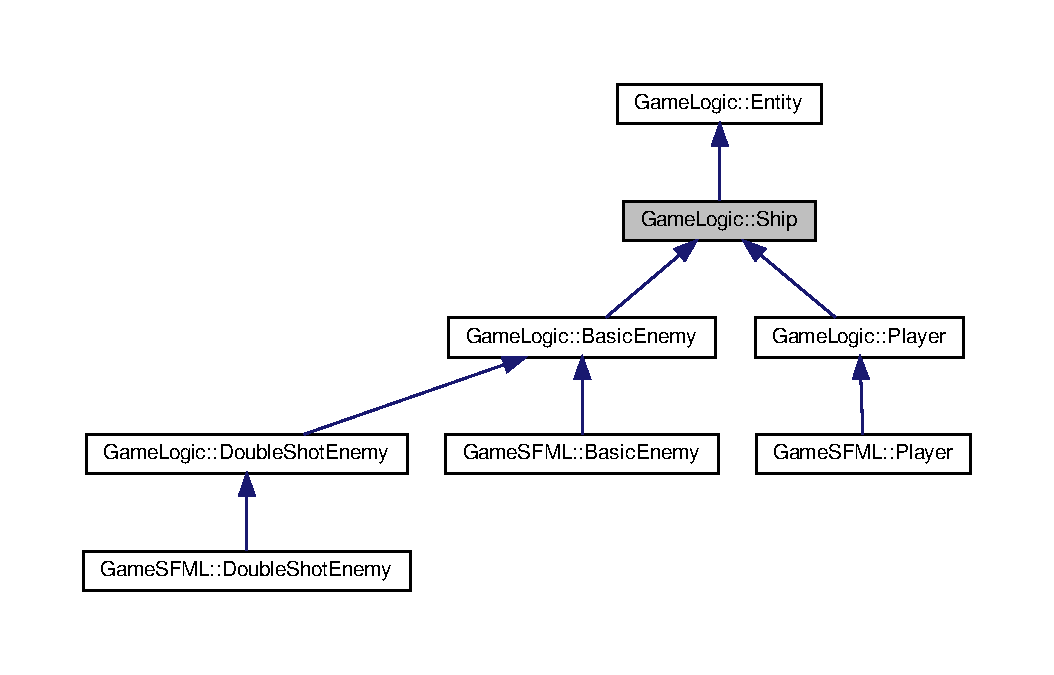
\includegraphics[width=350pt]{classGameLogic_1_1Ship__inherit__graph}
\end{center}
\end{figure}


Collaboration diagram for Game\+Logic\+:\+:Ship\+:
\nopagebreak
\begin{figure}[H]
\begin{center}
\leavevmode
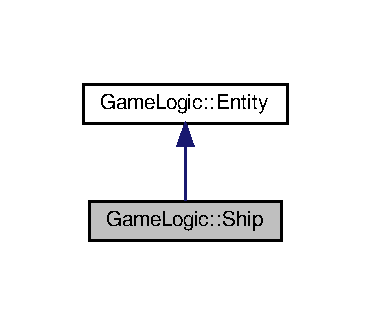
\includegraphics[width=178pt]{classGameLogic_1_1Ship__coll__graph}
\end{center}
\end{figure}
\subsection*{Public Member Functions}
\begin{DoxyCompactItemize}
\item 
\hyperlink{classGameLogic_1_1Ship_a2fabf559fb5b1f1c14c3da133bc42596}{Ship} (const pair$<$ int, int $>$ \&position, double width, double height, int health=1, double speed=1)
\begin{DoxyCompactList}\small\item\em Constructor of the \hyperlink{classGameLogic_1_1Ship}{Ship} class. \end{DoxyCompactList}\item 
virtual void \hyperlink{classGameLogic_1_1Ship_aaab731578b80b9e1920e3f2af2bc2f8c}{move} ()
\begin{DoxyCompactList}\small\item\em Virtual move function in \hyperlink{classGameLogic_1_1Ship}{Ship}. \end{DoxyCompactList}\item 
int \hyperlink{classGameLogic_1_1Ship_a5529646cead801dc8cc9d47f2f3d1d92}{get\+Health} () const
\begin{DoxyCompactList}\small\item\em Getter for the health of the ship. \end{DoxyCompactList}\item 
void \hyperlink{classGameLogic_1_1Ship_af0604b26727de4793a03464753ef443e}{set\+Health} (int health)
\begin{DoxyCompactList}\small\item\em Setter for the current health of the ship. \end{DoxyCompactList}\end{DoxyCompactItemize}
\subsection*{Additional Inherited Members}


\subsection{Detailed Description}
Class that represents all of the ships (enemies and player, even though player technically isn\textquotesingle{}t a ship) in game logic. 

\subsection{Constructor \& Destructor Documentation}
\mbox{\Hypertarget{classGameLogic_1_1Ship_a2fabf559fb5b1f1c14c3da133bc42596}\label{classGameLogic_1_1Ship_a2fabf559fb5b1f1c14c3da133bc42596}} 
\index{Game\+Logic\+::\+Ship@{Game\+Logic\+::\+Ship}!Ship@{Ship}}
\index{Ship@{Ship}!Game\+Logic\+::\+Ship@{Game\+Logic\+::\+Ship}}
\subsubsection{\texorpdfstring{Ship()}{Ship()}}
{\footnotesize\ttfamily Game\+Logic\+::\+Ship\+::\+Ship (\begin{DoxyParamCaption}\item[{const pair$<$ int, int $>$ \&}]{position,  }\item[{double}]{width,  }\item[{double}]{height,  }\item[{int}]{health = {\ttfamily 1},  }\item[{double}]{speed = {\ttfamily 1} }\end{DoxyParamCaption})}

Constructor of the \hyperlink{classGameLogic_1_1Ship}{Ship} class. 
\begin{DoxyParams}{Parameters}
{\em position} & position of the ship in the grid \\
\hline
{\em width} & width of the ship \\
\hline
{\em height} & height of the ship \\
\hline
{\em health} & health of the ship \\
\hline
{\em speed} & speed of the ship \\
\hline
\end{DoxyParams}


\subsection{Member Function Documentation}
\mbox{\Hypertarget{classGameLogic_1_1Ship_a5529646cead801dc8cc9d47f2f3d1d92}\label{classGameLogic_1_1Ship_a5529646cead801dc8cc9d47f2f3d1d92}} 
\index{Game\+Logic\+::\+Ship@{Game\+Logic\+::\+Ship}!get\+Health@{get\+Health}}
\index{get\+Health@{get\+Health}!Game\+Logic\+::\+Ship@{Game\+Logic\+::\+Ship}}
\subsubsection{\texorpdfstring{get\+Health()}{getHealth()}}
{\footnotesize\ttfamily int Game\+Logic\+::\+Ship\+::get\+Health (\begin{DoxyParamCaption}{ }\end{DoxyParamCaption}) const}

Getter for the health of the ship. \begin{DoxyReturn}{Returns}
The integer value representing the current health of the ship. 
\end{DoxyReturn}
\mbox{\Hypertarget{classGameLogic_1_1Ship_aaab731578b80b9e1920e3f2af2bc2f8c}\label{classGameLogic_1_1Ship_aaab731578b80b9e1920e3f2af2bc2f8c}} 
\index{Game\+Logic\+::\+Ship@{Game\+Logic\+::\+Ship}!move@{move}}
\index{move@{move}!Game\+Logic\+::\+Ship@{Game\+Logic\+::\+Ship}}
\subsubsection{\texorpdfstring{move()}{move()}}
{\footnotesize\ttfamily void Game\+Logic\+::\+Ship\+::move (\begin{DoxyParamCaption}{ }\end{DoxyParamCaption})\hspace{0.3cm}{\ttfamily [virtual]}}

Virtual move function in \hyperlink{classGameLogic_1_1Ship}{Ship}. 

Reimplemented in \hyperlink{classGameLogic_1_1BasicEnemy_a8c51b862c94953e5455c04c2227b6d73}{Game\+Logic\+::\+Basic\+Enemy}.

\mbox{\Hypertarget{classGameLogic_1_1Ship_af0604b26727de4793a03464753ef443e}\label{classGameLogic_1_1Ship_af0604b26727de4793a03464753ef443e}} 
\index{Game\+Logic\+::\+Ship@{Game\+Logic\+::\+Ship}!set\+Health@{set\+Health}}
\index{set\+Health@{set\+Health}!Game\+Logic\+::\+Ship@{Game\+Logic\+::\+Ship}}
\subsubsection{\texorpdfstring{set\+Health()}{setHealth()}}
{\footnotesize\ttfamily void Game\+Logic\+::\+Ship\+::set\+Health (\begin{DoxyParamCaption}\item[{int}]{health }\end{DoxyParamCaption})}

Setter for the current health of the ship. 
\begin{DoxyParams}{Parameters}
{\em health} & Integer value representing the new health of the ship. \\
\hline
\end{DoxyParams}


The documentation for this class was generated from the following files\+:\begin{DoxyCompactItemize}
\item 
Game\+Logic/\+Include/\+Game\+Logic/Ship.\+h\item 
Game\+Logic/src/Ship.\+cpp\end{DoxyCompactItemize}

\hypertarget{classGameLogic_1_1Stopwatch}{}\section{Game\+Logic\+:\+:Stopwatch Class Reference}
\label{classGameLogic_1_1Stopwatch}\index{Game\+Logic\+::\+Stopwatch@{Game\+Logic\+::\+Stopwatch}}


\hyperlink{classGameLogic_1_1Stopwatch}{Stopwatch} class to make sure the game runs at the same speed on every pc.  




{\ttfamily \#include $<$Stopwatch.\+h$>$}

\subsection*{Public Member Functions}
\begin{DoxyCompactItemize}
\item 
clock\+\_\+t \hyperlink{classGameLogic_1_1Stopwatch_a630ec6e48b90673127a033d18dd4d570}{get\+Start\+\_\+clock} () const
\begin{DoxyCompactList}\small\item\em Function returns when the clock was last started. \end{DoxyCompactList}\item 
void \hyperlink{classGameLogic_1_1Stopwatch_a8490b96964e128c93be7133e7a5386a5}{reset} ()
\begin{DoxyCompactList}\small\item\em Resets the clock. \end{DoxyCompactList}\item 
double \hyperlink{classGameLogic_1_1Stopwatch_a71ca51fb998fd7c16a64bf6f13ce8faa}{get\+Time\+Passed} ()
\begin{DoxyCompactList}\small\item\em Returns how much time has passed since the last time the clock was started. \end{DoxyCompactList}\end{DoxyCompactItemize}
\subsection*{Static Public Member Functions}
\begin{DoxyCompactItemize}
\item 
static shared\+\_\+ptr$<$ \hyperlink{classGameLogic_1_1Stopwatch}{Stopwatch} $>$ \hyperlink{classGameLogic_1_1Stopwatch_aaca0b7d8b21eb26ed2acb4cbd63fe208}{get\+Instance} ()
\begin{DoxyCompactList}\small\item\em Function to get the stopwatch instance. \end{DoxyCompactList}\end{DoxyCompactItemize}


\subsection{Detailed Description}
\hyperlink{classGameLogic_1_1Stopwatch}{Stopwatch} class to make sure the game runs at the same speed on every pc. Uses the singleton patterns. 

\subsection{Member Function Documentation}
\mbox{\Hypertarget{classGameLogic_1_1Stopwatch_aaca0b7d8b21eb26ed2acb4cbd63fe208}\label{classGameLogic_1_1Stopwatch_aaca0b7d8b21eb26ed2acb4cbd63fe208}} 
\index{Game\+Logic\+::\+Stopwatch@{Game\+Logic\+::\+Stopwatch}!get\+Instance@{get\+Instance}}
\index{get\+Instance@{get\+Instance}!Game\+Logic\+::\+Stopwatch@{Game\+Logic\+::\+Stopwatch}}
\subsubsection{\texorpdfstring{get\+Instance()}{getInstance()}}
{\footnotesize\ttfamily shared\+\_\+ptr$<$ \hyperlink{classGameLogic_1_1Stopwatch}{Stopwatch} $>$ Game\+Logic\+::\+Stopwatch\+::get\+Instance (\begin{DoxyParamCaption}{ }\end{DoxyParamCaption})\hspace{0.3cm}{\ttfamily [static]}}

Will return the stopwatch instance if one already exists, if not it will create one. \begin{DoxyReturn}{Returns}
The stopwatch instance 
\end{DoxyReturn}
\mbox{\Hypertarget{classGameLogic_1_1Stopwatch_a630ec6e48b90673127a033d18dd4d570}\label{classGameLogic_1_1Stopwatch_a630ec6e48b90673127a033d18dd4d570}} 
\index{Game\+Logic\+::\+Stopwatch@{Game\+Logic\+::\+Stopwatch}!get\+Start\+\_\+clock@{get\+Start\+\_\+clock}}
\index{get\+Start\+\_\+clock@{get\+Start\+\_\+clock}!Game\+Logic\+::\+Stopwatch@{Game\+Logic\+::\+Stopwatch}}
\subsubsection{\texorpdfstring{get\+Start\+\_\+clock()}{getStart\_clock()}}
{\footnotesize\ttfamily clock\+\_\+t Game\+Logic\+::\+Stopwatch\+::get\+Start\+\_\+clock (\begin{DoxyParamCaption}{ }\end{DoxyParamCaption}) const}

Function returns when the clock was last started. \begin{DoxyReturn}{Returns}
the time when the clock was last started. 
\end{DoxyReturn}
\mbox{\Hypertarget{classGameLogic_1_1Stopwatch_a71ca51fb998fd7c16a64bf6f13ce8faa}\label{classGameLogic_1_1Stopwatch_a71ca51fb998fd7c16a64bf6f13ce8faa}} 
\index{Game\+Logic\+::\+Stopwatch@{Game\+Logic\+::\+Stopwatch}!get\+Time\+Passed@{get\+Time\+Passed}}
\index{get\+Time\+Passed@{get\+Time\+Passed}!Game\+Logic\+::\+Stopwatch@{Game\+Logic\+::\+Stopwatch}}
\subsubsection{\texorpdfstring{get\+Time\+Passed()}{getTimePassed()}}
{\footnotesize\ttfamily double Game\+Logic\+::\+Stopwatch\+::get\+Time\+Passed (\begin{DoxyParamCaption}{ }\end{DoxyParamCaption})}

Returns how much time has passed since the last time the clock was started. \begin{DoxyReturn}{Returns}
how much time has passed 
\end{DoxyReturn}
\mbox{\Hypertarget{classGameLogic_1_1Stopwatch_a8490b96964e128c93be7133e7a5386a5}\label{classGameLogic_1_1Stopwatch_a8490b96964e128c93be7133e7a5386a5}} 
\index{Game\+Logic\+::\+Stopwatch@{Game\+Logic\+::\+Stopwatch}!reset@{reset}}
\index{reset@{reset}!Game\+Logic\+::\+Stopwatch@{Game\+Logic\+::\+Stopwatch}}
\subsubsection{\texorpdfstring{reset()}{reset()}}
{\footnotesize\ttfamily void Game\+Logic\+::\+Stopwatch\+::reset (\begin{DoxyParamCaption}{ }\end{DoxyParamCaption})}

Resets the clock. 

The documentation for this class was generated from the following files\+:\begin{DoxyCompactItemize}
\item 
Game\+Logic/\+Include/\+Game\+Logic/Stopwatch.\+h\item 
Game\+Logic/src/Stopwatch.\+cpp\item 
main.\+cpp\end{DoxyCompactItemize}

\hypertarget{classGameLogic_1_1Transformation}{}\section{Game\+Logic\+:\+:Transformation Class Reference}
\label{classGameLogic_1_1Transformation}\index{Game\+Logic\+::\+Transformation@{Game\+Logic\+::\+Transformation}}


Class used to convert from the game\+Logic grid to screen coordinates.  




{\ttfamily \#include $<$Transformation.\+h$>$}

\subsection*{Public Member Functions}
\begin{DoxyCompactItemize}
\item 
void \hyperlink{classGameLogic_1_1Transformation_a1a65e0d2527c3c558f5dfe59e0832d52}{set\+Screen\+Size} (unsigned int width, unsigned int height)
\begin{DoxyCompactList}\small\item\em Set the screen size used in calculating the correct screen coordinates. \end{DoxyCompactList}\item 
void \hyperlink{classGameLogic_1_1Transformation_a69686d5a12ba0e04b6ea7b80e5c874ac}{set\+X\+Min} (int x\+Min)
\begin{DoxyCompactList}\small\item\em Setter for the minimum value of the x value of the grid. \end{DoxyCompactList}\item 
void \hyperlink{classGameLogic_1_1Transformation_ac1818769a0212075fb865d0495ced12c}{set\+X\+Max} (int x\+Max)
\begin{DoxyCompactList}\small\item\em Setter for the maximum value of the x value of the grid. \end{DoxyCompactList}\item 
void \hyperlink{classGameLogic_1_1Transformation_a8863f56cd8d117a6817d288fa28258bd}{set\+Y\+Min} (int y\+Min)
\begin{DoxyCompactList}\small\item\em Setter for the minimum value of the y value of the grid. \end{DoxyCompactList}\item 
void \hyperlink{classGameLogic_1_1Transformation_a0da7509d874b735240aba51c72f31811}{set\+Y\+Max} (int y\+Max)
\begin{DoxyCompactList}\small\item\em Setter for the maximum value of the y value of the grid. \end{DoxyCompactList}\item 
pair$<$ double, double $>$ \hyperlink{classGameLogic_1_1Transformation_a30bed07a78fb248b129e50234ecef28a}{convert\+To\+Screen} (double X, double Y)
\begin{DoxyCompactList}\small\item\em Function to convert grid position (or between 2 grid positions) to screen coordinates. \end{DoxyCompactList}\item 
bool \hyperlink{classGameLogic_1_1Transformation_a573549aa64a0932387e9ab116e408493}{is\+In\+Grid} (pair$<$ int, int $>$ pos)
\begin{DoxyCompactList}\small\item\em Function checks whether a position is a valid grid position. \end{DoxyCompactList}\item 
double \hyperlink{classGameLogic_1_1Transformation_a1168354a2f68dcfcee917da9ec1076ac}{convert\+X\+To\+Screen} (double x)
\begin{DoxyCompactList}\small\item\em Convert a grid x coordinate to their screen equivalent. \end{DoxyCompactList}\item 
double \hyperlink{classGameLogic_1_1Transformation_a6a3d8fd76997ed12fc6dc9640118f405}{convert\+Y\+To\+Screen} (double y)
\begin{DoxyCompactList}\small\item\em Convert a grid y coordinate to their screen equivalent. \end{DoxyCompactList}\end{DoxyCompactItemize}
\subsection*{Static Public Member Functions}
\begin{DoxyCompactItemize}
\item 
static shared\+\_\+ptr$<$ \hyperlink{classGameLogic_1_1Transformation}{Transformation} $>$ \hyperlink{classGameLogic_1_1Transformation_a1b76a508913396581f4eeed63e96776d}{get\+Instance} ()
\begin{DoxyCompactList}\small\item\em Function to get the transformation instance. \end{DoxyCompactList}\end{DoxyCompactItemize}


\subsection{Detailed Description}
Class used to convert from the game\+Logic grid to screen coordinates. Uses the singleton pattern. 

\subsection{Member Function Documentation}
\mbox{\Hypertarget{classGameLogic_1_1Transformation_a30bed07a78fb248b129e50234ecef28a}\label{classGameLogic_1_1Transformation_a30bed07a78fb248b129e50234ecef28a}} 
\index{Game\+Logic\+::\+Transformation@{Game\+Logic\+::\+Transformation}!convert\+To\+Screen@{convert\+To\+Screen}}
\index{convert\+To\+Screen@{convert\+To\+Screen}!Game\+Logic\+::\+Transformation@{Game\+Logic\+::\+Transformation}}
\subsubsection{\texorpdfstring{convert\+To\+Screen()}{convertToScreen()}}
{\footnotesize\ttfamily pair$<$ double, double $>$ Game\+Logic\+::\+Transformation\+::convert\+To\+Screen (\begin{DoxyParamCaption}\item[{double}]{X,  }\item[{double}]{Y }\end{DoxyParamCaption})}

Function to convert grid position (or between 2 grid positions) to screen coordinates. 
\begin{DoxyParams}{Parameters}
{\em X} & the x value of the position you want to convert \\
\hline
{\em Y} & the y value of the position you want to convert \\
\hline
\end{DoxyParams}
\begin{DoxyReturn}{Returns}
the calculated screen position 
\end{DoxyReturn}
\mbox{\Hypertarget{classGameLogic_1_1Transformation_a1168354a2f68dcfcee917da9ec1076ac}\label{classGameLogic_1_1Transformation_a1168354a2f68dcfcee917da9ec1076ac}} 
\index{Game\+Logic\+::\+Transformation@{Game\+Logic\+::\+Transformation}!convert\+X\+To\+Screen@{convert\+X\+To\+Screen}}
\index{convert\+X\+To\+Screen@{convert\+X\+To\+Screen}!Game\+Logic\+::\+Transformation@{Game\+Logic\+::\+Transformation}}
\subsubsection{\texorpdfstring{convert\+X\+To\+Screen()}{convertXToScreen()}}
{\footnotesize\ttfamily double Game\+Logic\+::\+Transformation\+::convert\+X\+To\+Screen (\begin{DoxyParamCaption}\item[{double}]{x }\end{DoxyParamCaption})}

Convert a grid x coordinate to their screen equivalent. 
\begin{DoxyParams}{Parameters}
{\em x} & the x value to convert. \\
\hline
\end{DoxyParams}
\begin{DoxyReturn}{Returns}
the screen equivalent. 
\end{DoxyReturn}
\mbox{\Hypertarget{classGameLogic_1_1Transformation_a6a3d8fd76997ed12fc6dc9640118f405}\label{classGameLogic_1_1Transformation_a6a3d8fd76997ed12fc6dc9640118f405}} 
\index{Game\+Logic\+::\+Transformation@{Game\+Logic\+::\+Transformation}!convert\+Y\+To\+Screen@{convert\+Y\+To\+Screen}}
\index{convert\+Y\+To\+Screen@{convert\+Y\+To\+Screen}!Game\+Logic\+::\+Transformation@{Game\+Logic\+::\+Transformation}}
\subsubsection{\texorpdfstring{convert\+Y\+To\+Screen()}{convertYToScreen()}}
{\footnotesize\ttfamily double Game\+Logic\+::\+Transformation\+::convert\+Y\+To\+Screen (\begin{DoxyParamCaption}\item[{double}]{y }\end{DoxyParamCaption})}

Convert a grid y coordinate to their screen equivalent. 
\begin{DoxyParams}{Parameters}
{\em y} & the y value to convert. \\
\hline
\end{DoxyParams}
\begin{DoxyReturn}{Returns}
the screen equivalent. 
\end{DoxyReturn}
\mbox{\Hypertarget{classGameLogic_1_1Transformation_a1b76a508913396581f4eeed63e96776d}\label{classGameLogic_1_1Transformation_a1b76a508913396581f4eeed63e96776d}} 
\index{Game\+Logic\+::\+Transformation@{Game\+Logic\+::\+Transformation}!get\+Instance@{get\+Instance}}
\index{get\+Instance@{get\+Instance}!Game\+Logic\+::\+Transformation@{Game\+Logic\+::\+Transformation}}
\subsubsection{\texorpdfstring{get\+Instance()}{getInstance()}}
{\footnotesize\ttfamily shared\+\_\+ptr$<$ \hyperlink{classGameLogic_1_1Transformation}{Game\+Logic\+::\+Transformation} $>$ Game\+Logic\+::\+Transformation\+::get\+Instance (\begin{DoxyParamCaption}{ }\end{DoxyParamCaption})\hspace{0.3cm}{\ttfamily [static]}}

Will return the transformation instance if one already exists, if not it will create one. \begin{DoxyReturn}{Returns}
The transformation instance 
\end{DoxyReturn}
\mbox{\Hypertarget{classGameLogic_1_1Transformation_a573549aa64a0932387e9ab116e408493}\label{classGameLogic_1_1Transformation_a573549aa64a0932387e9ab116e408493}} 
\index{Game\+Logic\+::\+Transformation@{Game\+Logic\+::\+Transformation}!is\+In\+Grid@{is\+In\+Grid}}
\index{is\+In\+Grid@{is\+In\+Grid}!Game\+Logic\+::\+Transformation@{Game\+Logic\+::\+Transformation}}
\subsubsection{\texorpdfstring{is\+In\+Grid()}{isInGrid()}}
{\footnotesize\ttfamily bool Game\+Logic\+::\+Transformation\+::is\+In\+Grid (\begin{DoxyParamCaption}\item[{pair$<$ int, int $>$}]{pos }\end{DoxyParamCaption})}

Checks whether the recieved x and y values are between the grid\textquotesingle{}s max and min. 
\begin{DoxyParams}{Parameters}
{\em pos} & The position to check \\
\hline
\end{DoxyParams}
\begin{DoxyReturn}{Returns}
Boolean that is true when it\textquotesingle{}s a valid position. 
\end{DoxyReturn}
\mbox{\Hypertarget{classGameLogic_1_1Transformation_a1a65e0d2527c3c558f5dfe59e0832d52}\label{classGameLogic_1_1Transformation_a1a65e0d2527c3c558f5dfe59e0832d52}} 
\index{Game\+Logic\+::\+Transformation@{Game\+Logic\+::\+Transformation}!set\+Screen\+Size@{set\+Screen\+Size}}
\index{set\+Screen\+Size@{set\+Screen\+Size}!Game\+Logic\+::\+Transformation@{Game\+Logic\+::\+Transformation}}
\subsubsection{\texorpdfstring{set\+Screen\+Size()}{setScreenSize()}}
{\footnotesize\ttfamily void Game\+Logic\+::\+Transformation\+::set\+Screen\+Size (\begin{DoxyParamCaption}\item[{unsigned int}]{width,  }\item[{unsigned int}]{height }\end{DoxyParamCaption})}

Set the screen size used in calculating the correct screen coordinates. 
\begin{DoxyParams}{Parameters}
{\em width} & the width of the screen. \\
\hline
{\em height} & the height of the screen. \\
\hline
\end{DoxyParams}
\mbox{\Hypertarget{classGameLogic_1_1Transformation_ac1818769a0212075fb865d0495ced12c}\label{classGameLogic_1_1Transformation_ac1818769a0212075fb865d0495ced12c}} 
\index{Game\+Logic\+::\+Transformation@{Game\+Logic\+::\+Transformation}!set\+X\+Max@{set\+X\+Max}}
\index{set\+X\+Max@{set\+X\+Max}!Game\+Logic\+::\+Transformation@{Game\+Logic\+::\+Transformation}}
\subsubsection{\texorpdfstring{set\+X\+Max()}{setXMax()}}
{\footnotesize\ttfamily void Game\+Logic\+::\+Transformation\+::set\+X\+Max (\begin{DoxyParamCaption}\item[{int}]{x\+Max }\end{DoxyParamCaption})}

Setter for the maximum value of the x value of the grid. Used if you want to change the grid mid game. 
\begin{DoxyParams}{Parameters}
{\em x\+Min} & the new x maximum. \\
\hline
\end{DoxyParams}
\mbox{\Hypertarget{classGameLogic_1_1Transformation_a69686d5a12ba0e04b6ea7b80e5c874ac}\label{classGameLogic_1_1Transformation_a69686d5a12ba0e04b6ea7b80e5c874ac}} 
\index{Game\+Logic\+::\+Transformation@{Game\+Logic\+::\+Transformation}!set\+X\+Min@{set\+X\+Min}}
\index{set\+X\+Min@{set\+X\+Min}!Game\+Logic\+::\+Transformation@{Game\+Logic\+::\+Transformation}}
\subsubsection{\texorpdfstring{set\+X\+Min()}{setXMin()}}
{\footnotesize\ttfamily void Game\+Logic\+::\+Transformation\+::set\+X\+Min (\begin{DoxyParamCaption}\item[{int}]{x\+Min }\end{DoxyParamCaption})}

Setter for the minimum value of the x value of the grid. Used if you want to change the grid mid game. 
\begin{DoxyParams}{Parameters}
{\em x\+Min} & the new x minimum. \\
\hline
\end{DoxyParams}
\mbox{\Hypertarget{classGameLogic_1_1Transformation_a0da7509d874b735240aba51c72f31811}\label{classGameLogic_1_1Transformation_a0da7509d874b735240aba51c72f31811}} 
\index{Game\+Logic\+::\+Transformation@{Game\+Logic\+::\+Transformation}!set\+Y\+Max@{set\+Y\+Max}}
\index{set\+Y\+Max@{set\+Y\+Max}!Game\+Logic\+::\+Transformation@{Game\+Logic\+::\+Transformation}}
\subsubsection{\texorpdfstring{set\+Y\+Max()}{setYMax()}}
{\footnotesize\ttfamily void Game\+Logic\+::\+Transformation\+::set\+Y\+Max (\begin{DoxyParamCaption}\item[{int}]{y\+Max }\end{DoxyParamCaption})}

Setter for the maximum value of the y value of the grid. Used if you want to change the grid mid game. 
\begin{DoxyParams}{Parameters}
{\em x\+Min} & the new y maximum. \\
\hline
\end{DoxyParams}
\mbox{\Hypertarget{classGameLogic_1_1Transformation_a8863f56cd8d117a6817d288fa28258bd}\label{classGameLogic_1_1Transformation_a8863f56cd8d117a6817d288fa28258bd}} 
\index{Game\+Logic\+::\+Transformation@{Game\+Logic\+::\+Transformation}!set\+Y\+Min@{set\+Y\+Min}}
\index{set\+Y\+Min@{set\+Y\+Min}!Game\+Logic\+::\+Transformation@{Game\+Logic\+::\+Transformation}}
\subsubsection{\texorpdfstring{set\+Y\+Min()}{setYMin()}}
{\footnotesize\ttfamily void Game\+Logic\+::\+Transformation\+::set\+Y\+Min (\begin{DoxyParamCaption}\item[{int}]{y\+Min }\end{DoxyParamCaption})}

Setter for the minimum value of the y value of the grid. Used if you want to change the grid mid game. 
\begin{DoxyParams}{Parameters}
{\em x\+Min} & the new y minimum. \\
\hline
\end{DoxyParams}


The documentation for this class was generated from the following files\+:\begin{DoxyCompactItemize}
\item 
Game\+Logic/\+Include/\+Game\+Logic/Transformation.\+h\item 
Game\+Logic/src/Transformation.\+cpp\item 
main.\+cpp\end{DoxyCompactItemize}

%--- End generated contents ---

% Index
\backmatter
\newpage
\phantomsection
\clearemptydoublepage
\addcontentsline{toc}{chapter}{Index}
\printindex

\end{document}
